\documentclass[8pt,aspectratio=1610]{beamer}
\usepackage[utf8]{inputenc}
\usepackage{booktabs}
\usepackage{array}
\usepackage{graphicx}
\usepackage{xcolor}
\usepackage{tikz}
\usetikzlibrary{positioning,arrows.meta,decorations.pathreplacing,calc,shadows}
\usepackage{pgfplots}
\pgfplotsset{compat=1.18}
\usepackage{amsmath}
\usepackage{amssymb}
\usepackage{amsfonts}
\usepackage{algorithm}
\usepackage{algorithmic}

\usetheme{metropolis}
\usecolortheme{wolverine}
\metroset{progressbar=frametitle,block=fill}
\setbeamertemplate{navigation symbols}{}

% Define custom colors complementing the Wolverine theme
\definecolor{maizelight}{RGB}{255, 203, 5}
\definecolor{maizedark}{RGB}{255, 167, 0}
\definecolor{bluelight}{RGB}{0, 39, 76}
\definecolor{tealaccent}{RGB}{0, 128, 128}
\definecolor{orangeaccent}{RGB}{255, 138, 51}

% Customize block colors
\setbeamercolor{block title}{bg=bluelight,fg=white}
\setbeamercolor{block body}{bg=bluelight!10,fg=black}
\setbeamercolor{block title example}{bg=maizelight,fg=black}
\setbeamercolor{block body example}{bg=maizelight!15,fg=black}
\setbeamercolor{block title alerted}{bg=orangeaccent,fg=white}
\setbeamercolor{block body alerted}{bg=orangeaccent!15,fg=black}

% Custom block environments
\newenvironment<>{techblock}[1]{%
  \setbeamercolor{block title}{bg=tealaccent,fg=white}%
  \setbeamercolor{block body}{bg=tealaccent!10,fg=black}%
  \begin{block}#2{#1}}{\end{block}}

\newenvironment<>{tipblock}[1]{%
  \setbeamercolor{block title}{bg=maizedark,fg=black}%
  \setbeamercolor{block body}{bg=maizedark!15,fg=black}%
  \begin{block}#2{#1}}{\end{block}}

% Title slide information
\title{Clustering}
\subtitle{CMSC 173 - Machine Learning}
\author{Noel Jeffrey Pinton}
\institute{Department of Computer Science\\University of the Philippines - Cebu}
\date{\today}

\begin{document}

\begin{frame}
\titlepage
\end{frame}

\begin{frame}{Outline}
\tableofcontents
\end{frame}

% ========================================
% Section: Introduction
% ========================================

\section{Introduction \& Motivation}

\begin{frame}{What is Clustering?}
\begin{columns}[t]
\begin{column}{0.48\textwidth}
\begin{block}{Definition}
\textbf{Clustering} is the task of grouping a set of objects such that objects in the same group (cluster) are more similar to each other than to those in other groups.
\end{block}

\vspace{0.2cm}

\begin{exampleblock}{Key Characteristics}
\begin{itemize}
\setlength{\itemsep}{2pt}
\item Unsupervised learning
\item No labeled data required
\item Discover hidden patterns
\item Data-driven groupings
\end{itemize}
\end{exampleblock}
\end{column}

\begin{column}{0.48\textwidth}
\centering
\vspace{0pt}
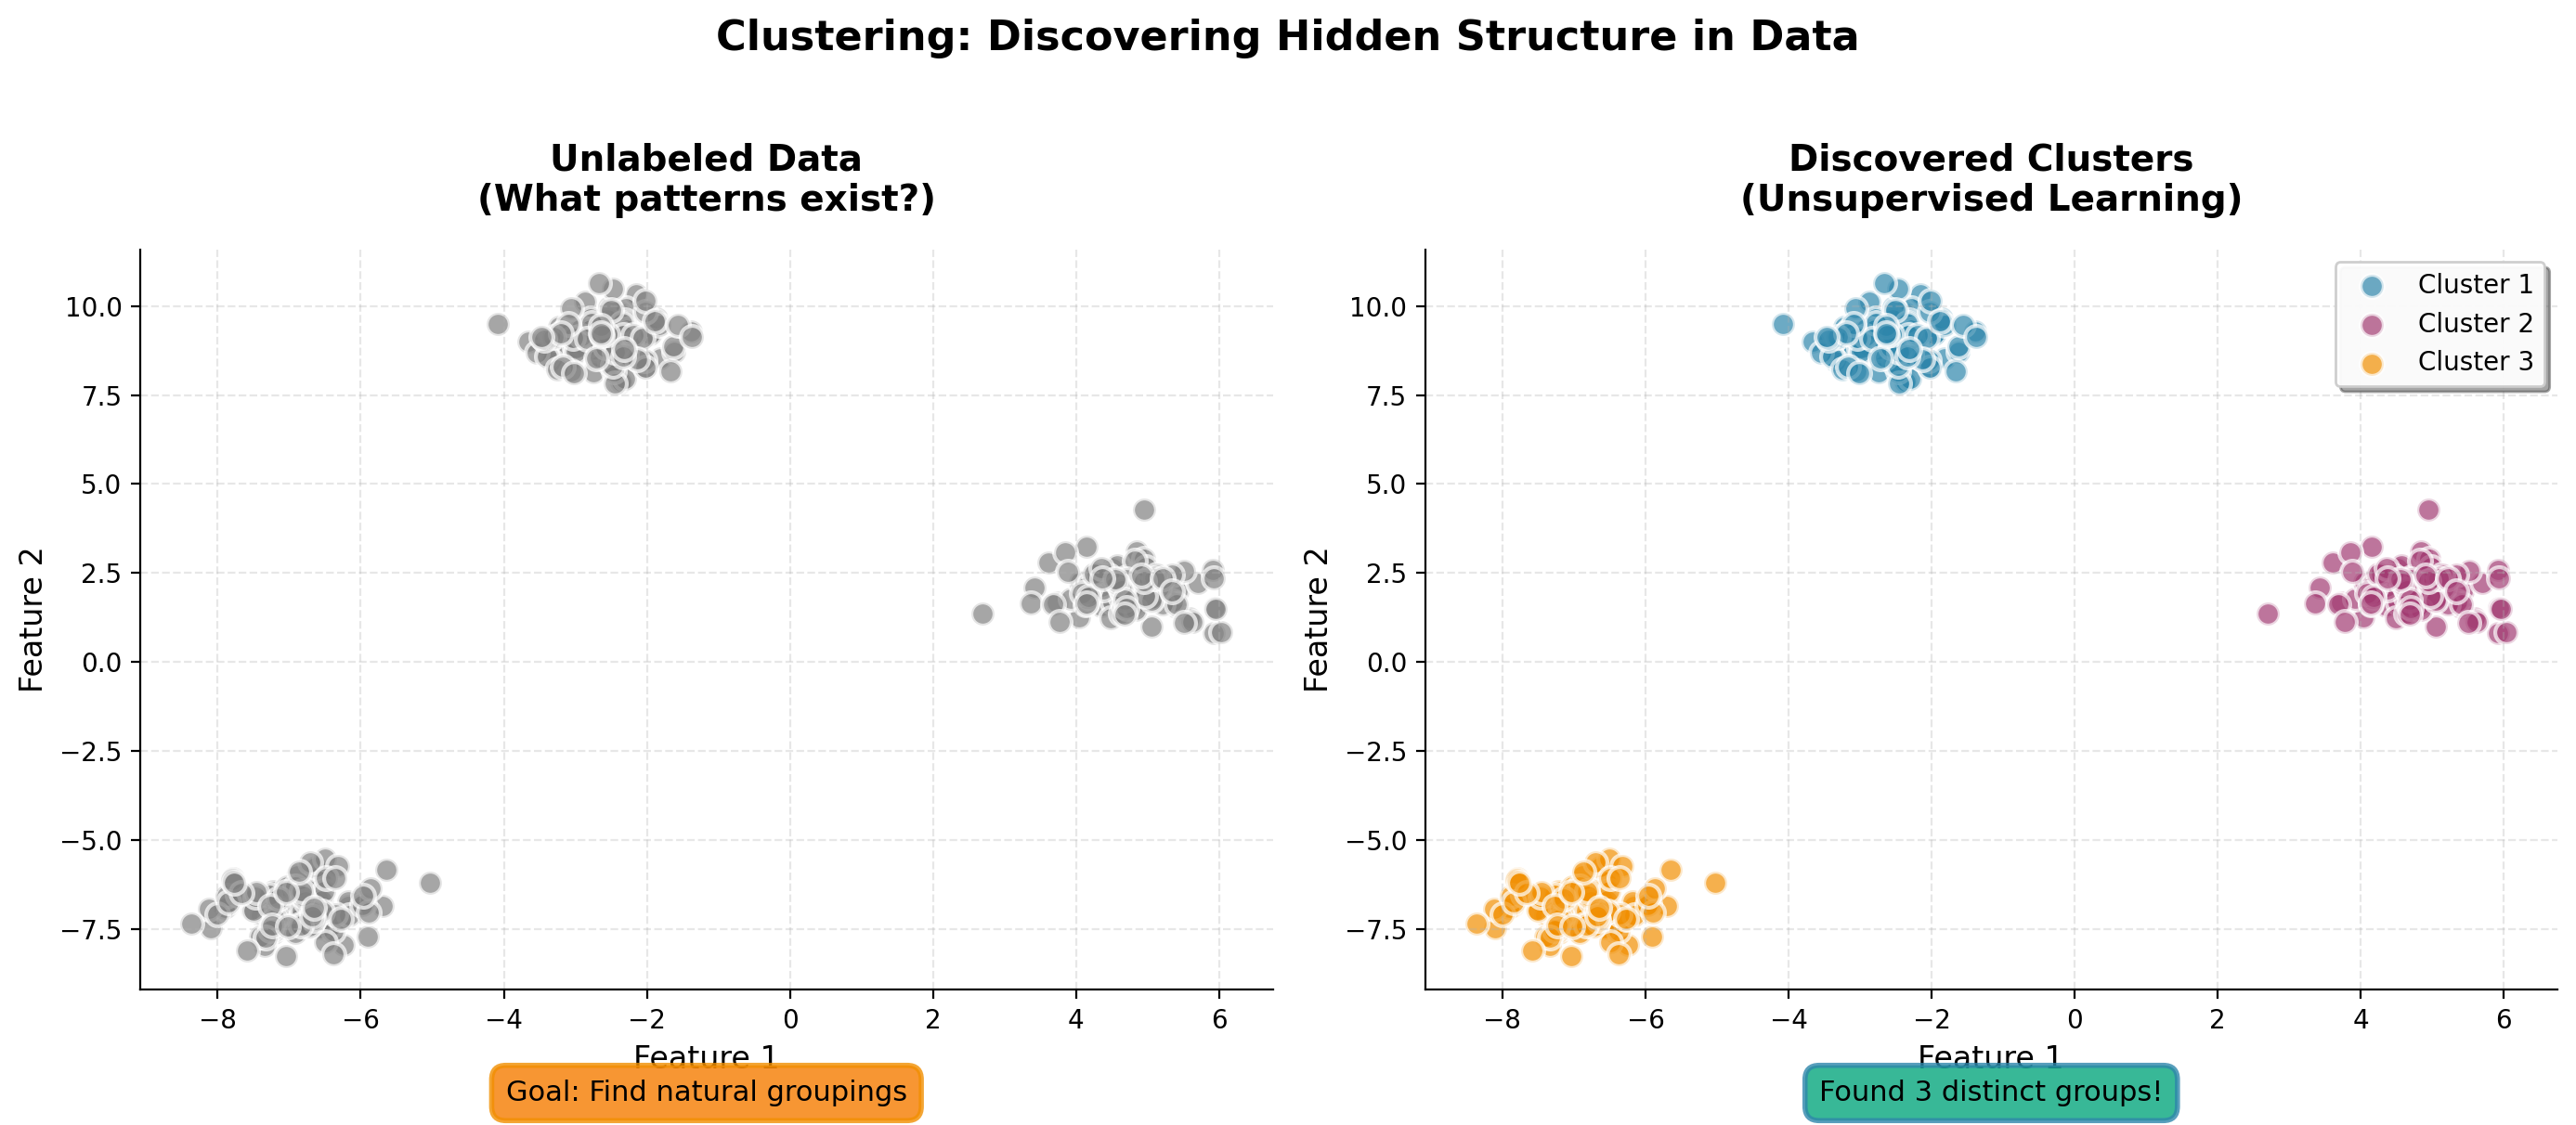
\includegraphics[width=\textwidth]{../figures/clustering_motivation.png}
\end{column}
\end{columns}

\vspace{0.03cm}

\begin{alertblock}{Goal}
Find natural groupings in data without prior knowledge of group labels.
\end{alertblock}
\end{frame}

\begin{frame}{Supervised vs Unsupervised Learning}
\begin{columns}[t]
\begin{column}{0.48\textwidth}
\begin{block}{Supervised Learning}
\begin{itemize}
\setlength{\itemsep}{2pt}
\item Training data has \textbf{labels}
\item Learn mapping: $f: X \rightarrow Y$
\item Goal: Predict labels for new data
\item Examples: Classification, regression
\end{itemize}
\end{block}

\vspace{0.2cm}

\textbf{Example:}
\begin{itemize}
\item Input: Email text
\item Label: Spam/Not Spam
\item Task: Learn to classify
\end{itemize}
\end{column}

\begin{column}{0.48\textwidth}
\begin{block}{Unsupervised Learning}
\begin{itemize}
\setlength{\itemsep}{2pt}
\item Training data has \textbf{no labels}
\item Discover structure in $X$
\item Goal: Find patterns, groups
\item Examples: Clustering, dimensionality reduction
\end{itemize}
\end{block}

\vspace{0.2cm}

\textbf{Example:}
\begin{itemize}
\item Input: Customer purchase data
\item No labels
\item Task: Find customer segments
\end{itemize}
\end{column}
\end{columns}

\vspace{0.05cm}

\begin{alertblock}{Clustering = Unsupervised}
We discover groups without knowing what they should be in advance.
\end{alertblock}
\end{frame}

\begin{frame}{Real-World Applications}
\begin{columns}[t]
\begin{column}{0.48\textwidth}
\begin{block}{Business \& Marketing}
\begin{itemize}
\setlength{\itemsep}{2pt}
\item \textbf{Customer segmentation}: Group customers by behavior
\item \textbf{Market research}: Identify consumer groups
\item \textbf{Recommendation systems}: Group similar items
\end{itemize}
\end{block}

\vspace{0.15cm}

\begin{block}{Biology \& Medicine}
\begin{itemize}
\setlength{\itemsep}{2pt}
\item \textbf{Gene expression}: Find related genes
\item \textbf{Disease diagnosis}: Identify patient subgroups
\item \textbf{Protein structure}: Analyze protein families
\end{itemize}
\end{block}
\end{column}

\begin{column}{0.48\textwidth}
\begin{block}{Image \& Vision}
\begin{itemize}
\setlength{\itemsep}{2pt}
\item \textbf{Image segmentation}: Group pixels by similarity
\item \textbf{Object recognition}: Cluster visual features
\item \textbf{Color quantization}: Reduce color palette
\end{itemize}
\end{block}

\vspace{0.15cm}

\begin{block}{Text \& Web}
\begin{itemize}
\setlength{\itemsep}{2pt}
\item \textbf{Document clustering}: Group similar documents
\item \textbf{Topic modeling}: Discover themes
\item \textbf{Social network analysis}: Find communities
\end{itemize}
\end{block}
\end{column}
\end{columns}

\vspace{0.05cm}

\begin{alertblock}{Common Theme}
All involve finding structure in unlabeled data!
\end{alertblock}
\end{frame}

\begin{frame}{Types of Clustering}
\begin{columns}[t]
\begin{column}{0.48\textwidth}
\begin{block}{Partitional Clustering}
\begin{itemize}
\setlength{\itemsep}{2pt}
\item Divide data into \textbf{K} non-overlapping groups
\item Each point belongs to exactly \textbf{one} cluster
\item Flat structure
\item Examples: K-Means, K-Medoids, GMM
\end{itemize}
\end{block}

\vspace{0.2cm}

\textbf{Characteristics:}
\begin{itemize}
\item Need to specify K
\item Fast and scalable
\item Sensitive to initialization
\end{itemize}
\end{column}

\begin{column}{0.48\textwidth}
\begin{block}{Hierarchical Clustering}
\begin{itemize}
\setlength{\itemsep}{2pt}
\item Build a \textbf{tree} of clusters (dendrogram)
\item Can extract K clusters at any level
\item Nested structure
\item Examples: Agglomerative, Divisive
\end{itemize}
\end{block}

\vspace{0.2cm}

\textbf{Characteristics:}
\begin{itemize}
\item No need to specify K upfront
\item More interpretable hierarchy
\item Computationally expensive
\end{itemize}
\end{column}
\end{columns}

\vspace{0.1cm}

\begin{alertblock}{This Lecture}
Focus on \textbf{Partitional} (K-Means, GMM) and \textbf{Hierarchical} methods.
\end{alertblock}
\end{frame}

% ========================================
% Section: Distance Metrics
% ========================================

\section{Foundation: Distance \& Similarity}

\begin{frame}{Distance Metrics}

\begin{block}{Common Distance Metrics}
For $\mathbf{x} = (x_1, \ldots, x_d)$ and $\mathbf{y} = (y_1, \ldots, y_d)$:

\vspace{0.1cm}

\begin{columns}[T]
\begin{column}{0.48\textwidth}
\textbf{1. Euclidean Distance} (L2)
$$d(\mathbf{x}, \mathbf{y}) = \sqrt{\sum_{i=1}^{d} (x_i - y_i)^2}$$

\textbf{2. Manhattan Distance} (L1)
$$d(\mathbf{x}, \mathbf{y}) = \sum_{i=1}^{d} |x_i - y_i|$$
\end{column}

\begin{column}{0.48\textwidth}
\textbf{3. Chebyshev Distance} (L$\infty$)
$$d(\mathbf{x}, \mathbf{y}) = \max_{i} |x_i - y_i|$$

\textbf{4. Cosine Similarity}
$$\text{sim}(\mathbf{x}, \mathbf{y}) = \frac{\mathbf{x} \cdot \mathbf{y}}{\|\mathbf{x}\| \|\mathbf{y}\|}$$
\end{column}
\end{columns}
\end{block}

\vspace{0.1cm}

\centering
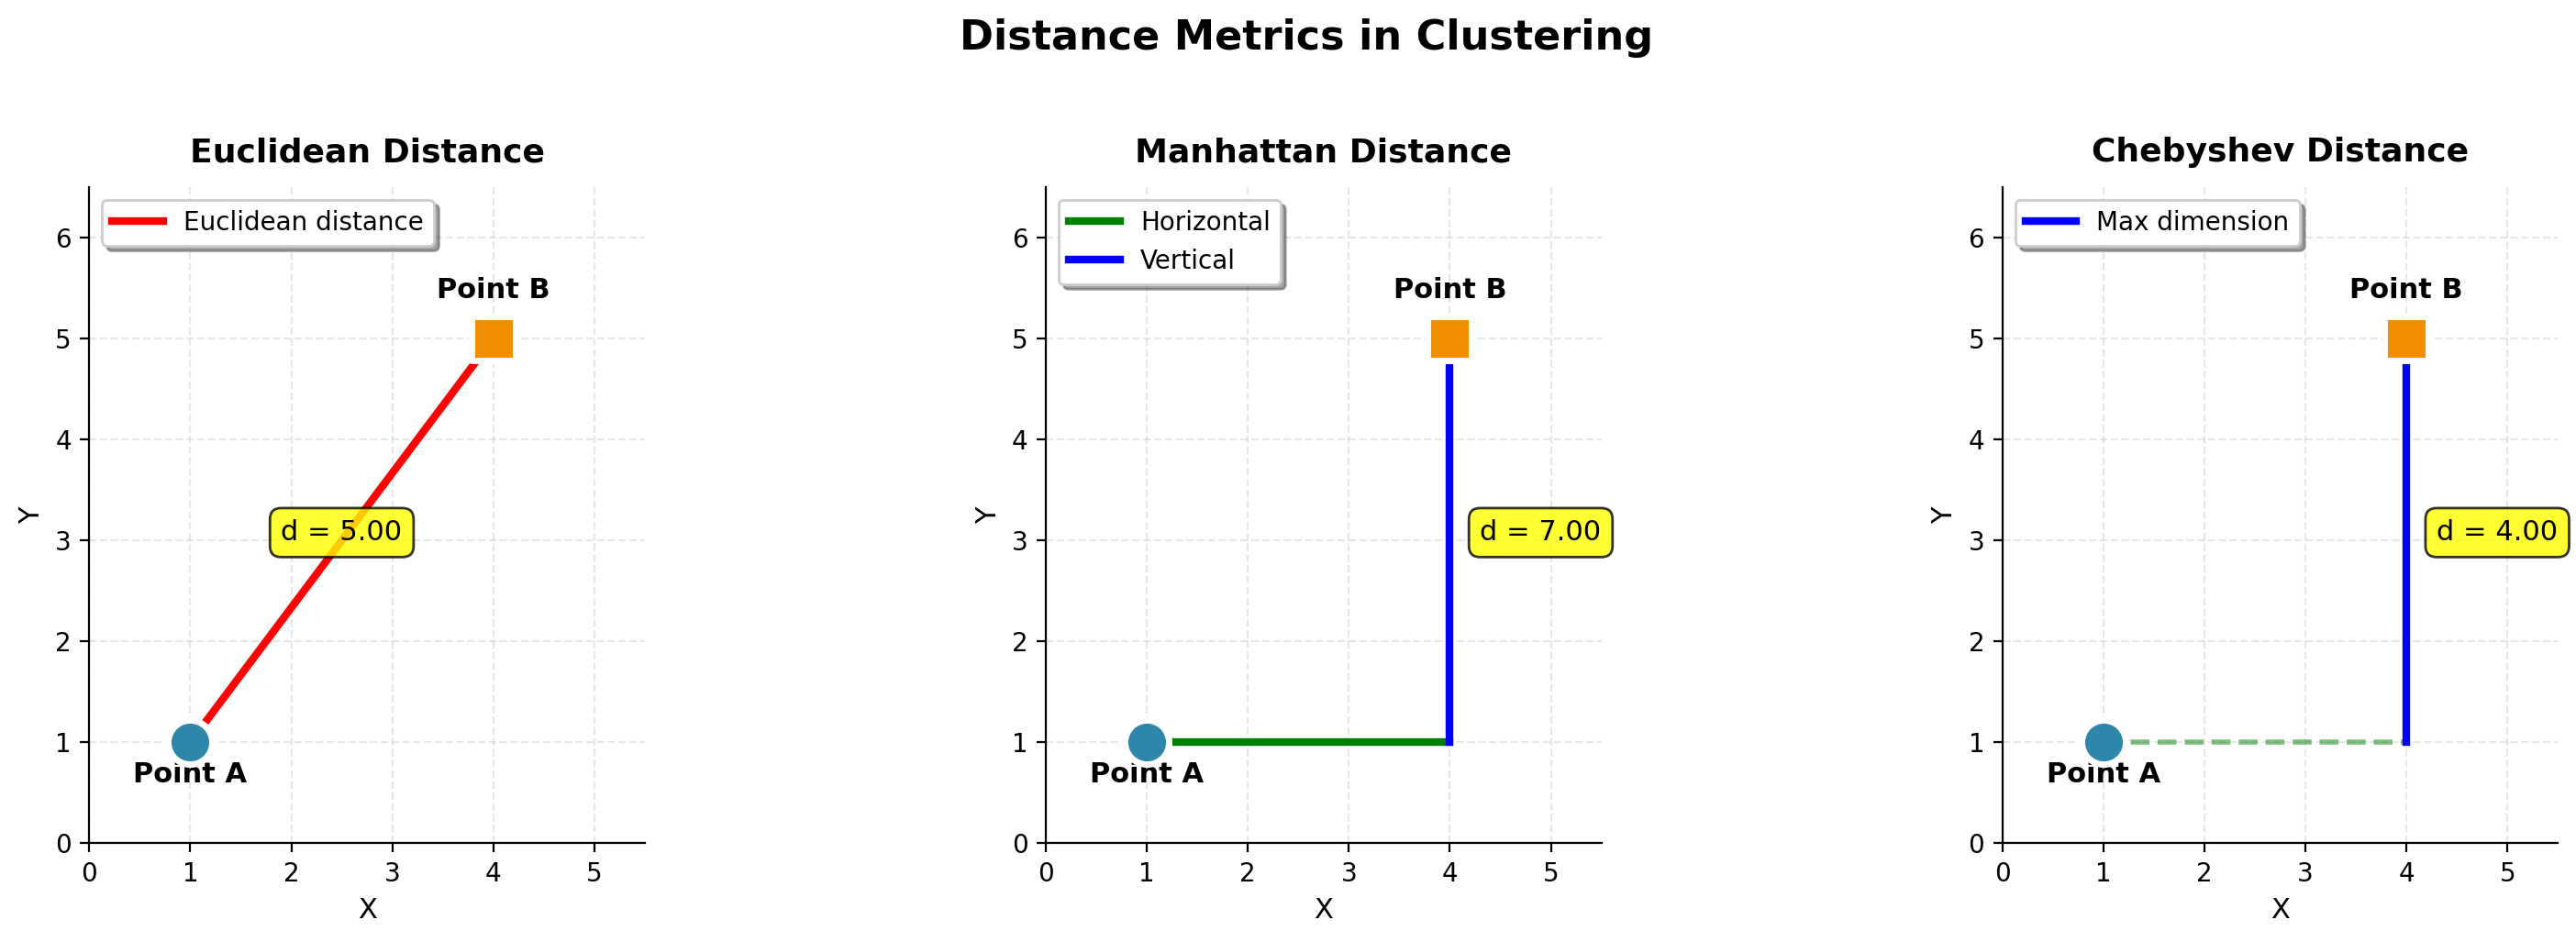
\includegraphics[width=0.75\textwidth]{../figures/distance_metrics.png}
\end{frame}

\begin{frame}{Properties of Distance Metrics}
\textbf{A valid distance metric must satisfy:}

\vspace{0.2cm}

\begin{block}{Metric Axioms}
For all points $\mathbf{x}, \mathbf{y}, \mathbf{z}$:

\vspace{0.1cm}

\begin{enumerate}
\setlength{\itemsep}{3pt}
\item \textbf{Non-negativity}: $d(\mathbf{x}, \mathbf{y}) \geq 0$
\item \textbf{Identity}: $d(\mathbf{x}, \mathbf{y}) = 0 \iff \mathbf{x} = \mathbf{y}$
\item \textbf{Symmetry}: $d(\mathbf{x}, \mathbf{y}) = d(\mathbf{y}, \mathbf{x})$
\item \textbf{Triangle inequality}: $d(\mathbf{x}, \mathbf{z}) \leq d(\mathbf{x}, \mathbf{y}) + d(\mathbf{y}, \mathbf{z})$
\end{enumerate}
\end{block}

\vspace{0.2cm}

\begin{exampleblock}{Choosing the Right Metric}
\begin{itemize}
\setlength{\itemsep}{2pt}
\item \textbf{Euclidean}: Most common, assumes all features equally important
\item \textbf{Manhattan}: Less sensitive to outliers, good for high dimensions
\item \textbf{Cosine}: Good for text/document clustering (direction matters)
\item \textbf{Custom}: Domain-specific distances (e.g., edit distance for strings)
\end{itemize}
\end{exampleblock}
\end{frame}

% ========================================
% Section: K-Means Clustering
% ========================================

\section{Partitional Clustering: K-Means}

\begin{frame}{K-Means Algorithm: Overview}

\begin{columns}[T]
\begin{column}{0.45\textwidth}
\begin{alertblock}{Goal}
Partition $n$ points into $K$ clusters
\end{alertblock}

\vspace{0.1cm}

\begin{block}{Key Idea}
\begin{itemize}
\setlength{\itemsep}{1pt}
\item Each cluster has \textbf{centroid} (mean)
\item Assign points to \textbf{nearest} centroid
\item Update centroids iteratively
\item Minimize within-cluster variance
\end{itemize}
\end{block}

\vspace{0.1cm}

\begin{exampleblock}{Input \& Output}
\textbf{Input:}
\begin{itemize}
\setlength{\itemsep}{0pt}
\item Dataset $X$, Number $K$
\end{itemize}

\textbf{Output:}
\begin{itemize}
\setlength{\itemsep}{0pt}
\item Assignments $\{C_1, \ldots, C_K\}$
\item Centroids $\{\boldsymbol{\mu}_1, \ldots, \boldsymbol{\mu}_K\}$
\end{itemize}
\end{exampleblock}
\end{column}

\begin{column}{0.52\textwidth}
\centering
\vspace{0pt}
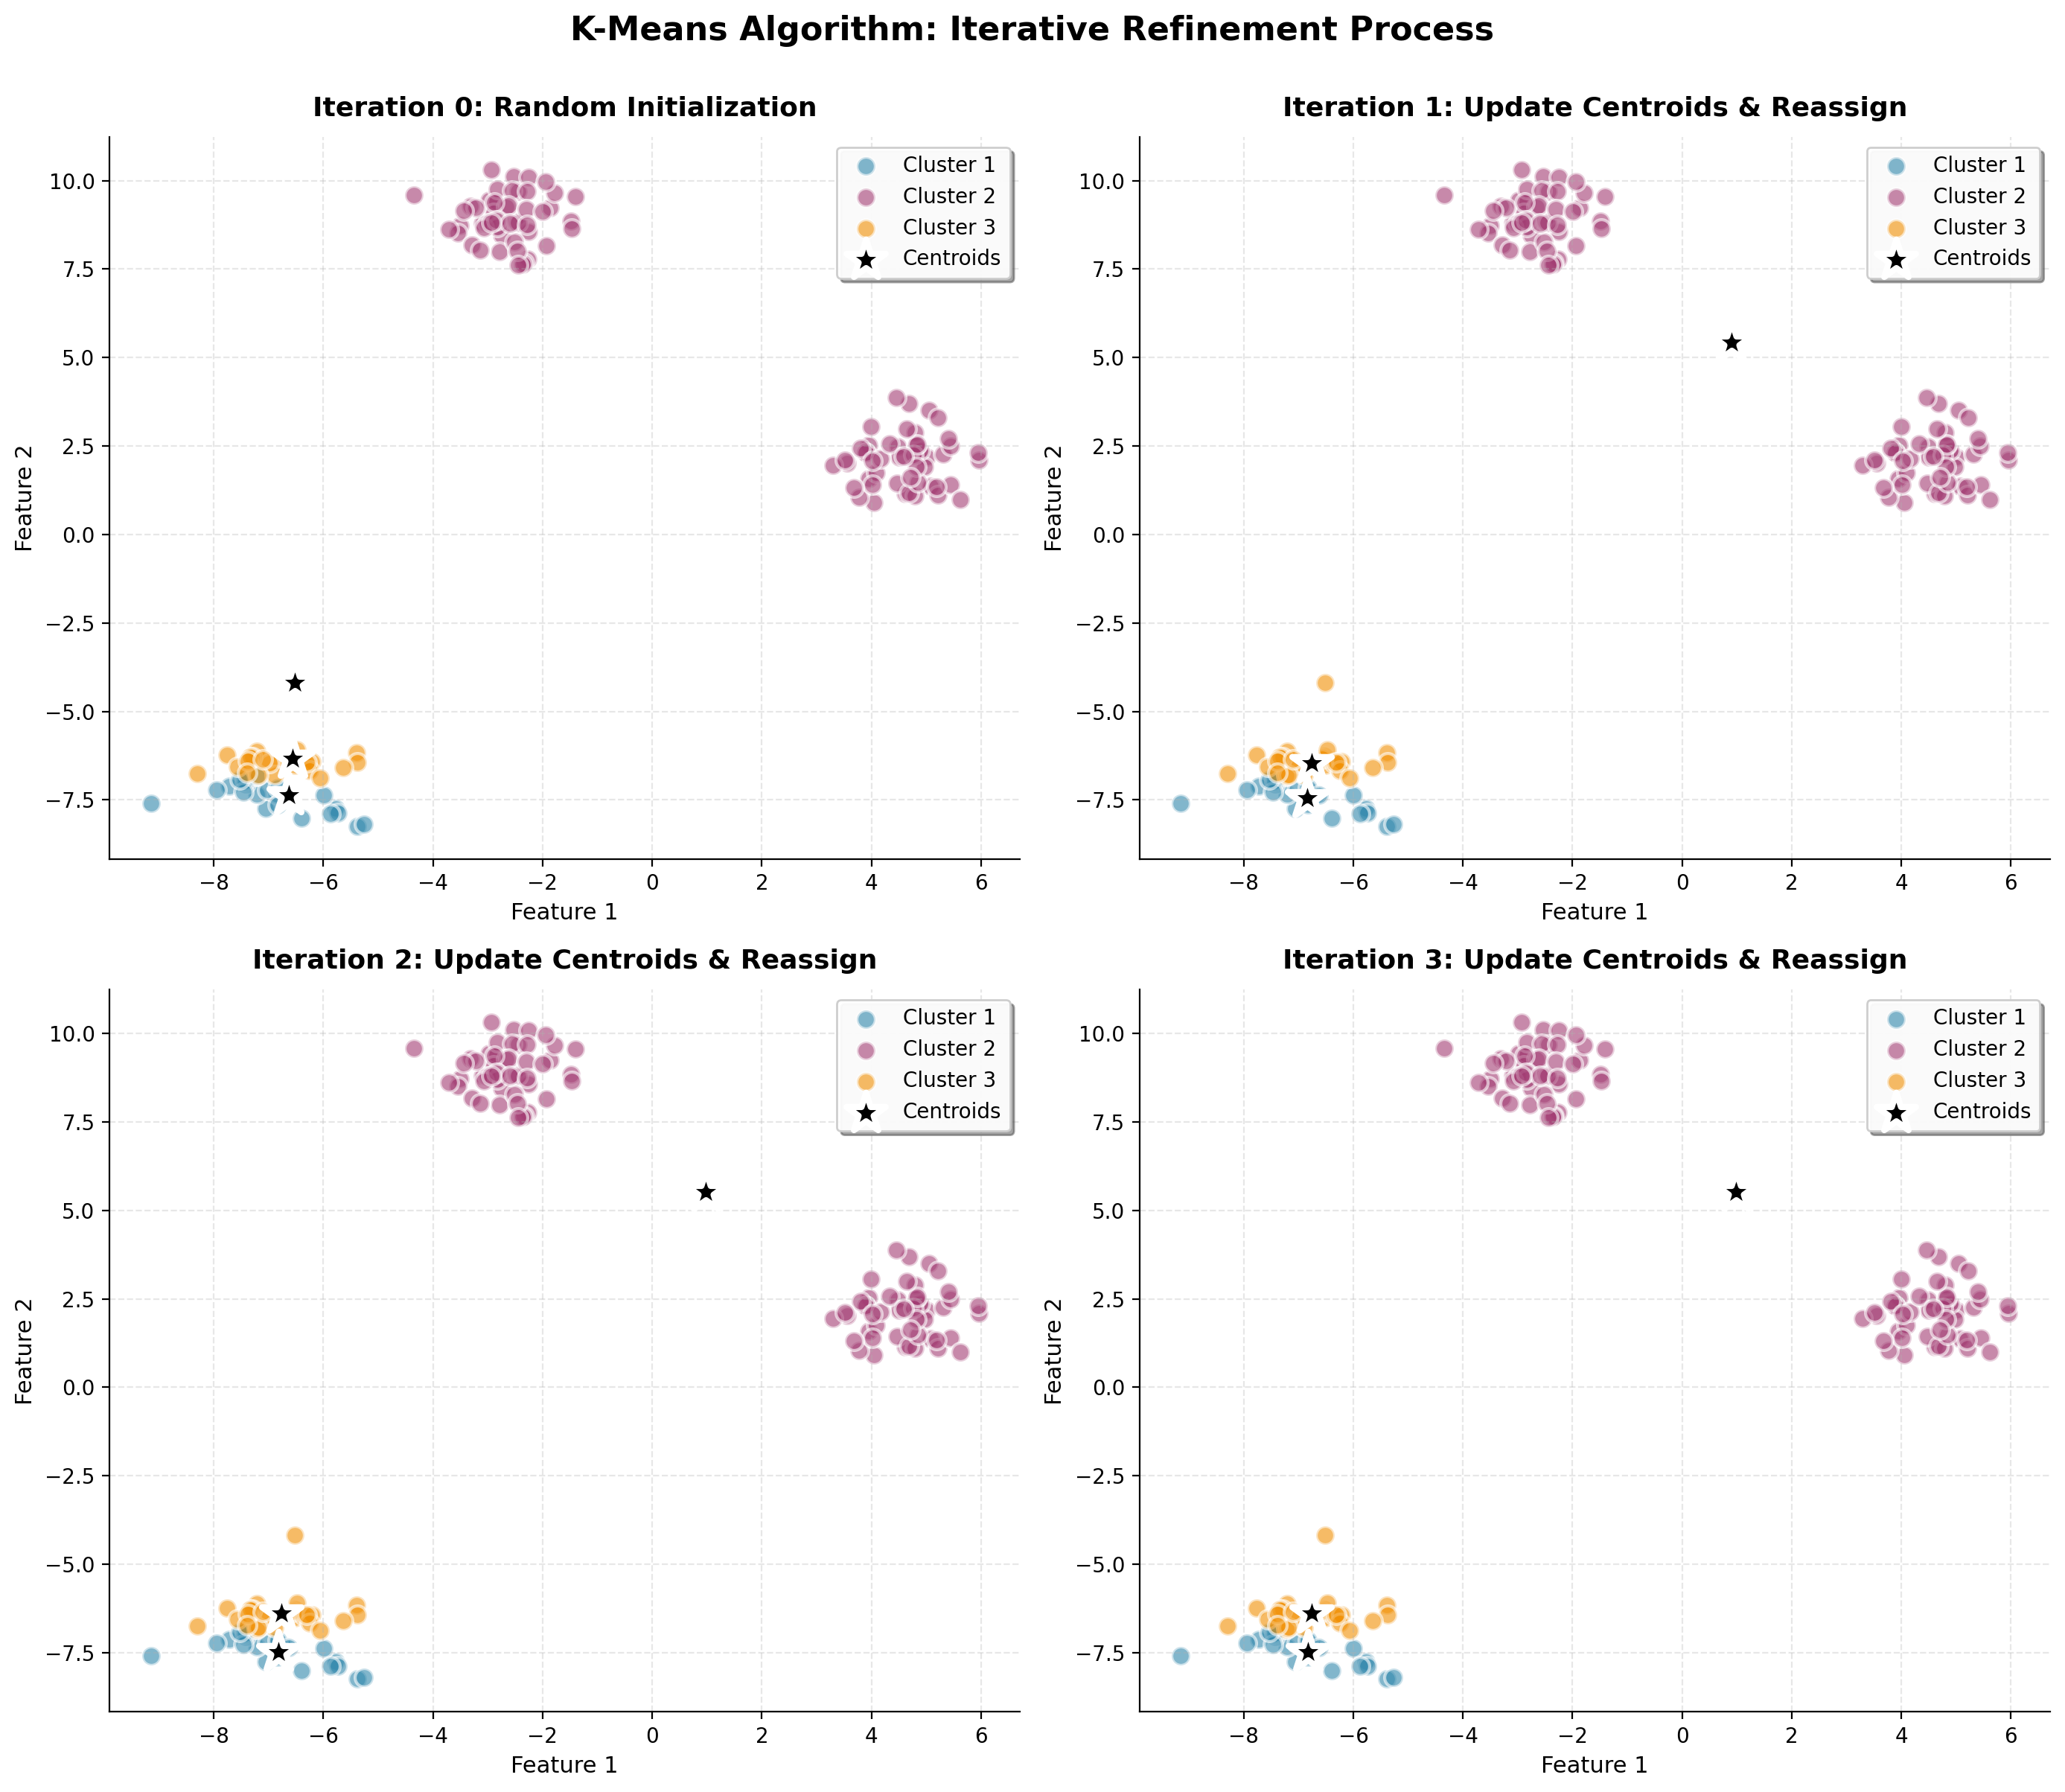
\includegraphics[width=\textwidth]{../figures/kmeans_iterations.png}
\end{column}
\end{columns}
\end{frame}

\begin{frame}{K-Means Objective Function}
\textbf{Minimize within-cluster sum of squares (WCSS):}

\vspace{0.2cm}

\begin{block}{Objective}
$$J = \sum_{k=1}^{K} \sum_{\mathbf{x}_i \in C_k} \|\mathbf{x}_i - \boldsymbol{\mu}_k\|^2$$

where:
\begin{itemize}
\item $C_k$ = set of points in cluster $k$
\item $\boldsymbol{\mu}_k$ = centroid of cluster $k$
\item $\|\cdot\|$ = Euclidean distance
\end{itemize}
\end{block}

\vspace{0.15cm}

\begin{exampleblock}{Interpretation}
\begin{itemize}
\setlength{\itemsep}{2pt}
\item Minimize total squared distance from points to their centroids
\item Encourages \textbf{compact}, \textbf{spherical} clusters
\item Also called \textbf{inertia} or \textbf{distortion}
\item NP-hard to minimize globally, but heuristics work well
\end{itemize}
\end{exampleblock}

\vspace{0.1cm}

\begin{alertblock}{Note}
K-Means finds \textbf{local minimum}, not necessarily global!
\end{alertblock}
\end{frame}

\begin{frame}[fragile]{K-Means Algorithm (Lloyd's Algorithm)}
\begin{algorithm}[H]
\caption{K-Means Clustering}
\begin{algorithmic}[1]
\REQUIRE Dataset $X = \{\mathbf{x}_1, \ldots, \mathbf{x}_n\}$, number of clusters $K$
\ENSURE Cluster assignments and centroids

\STATE \textbf{Initialize} $K$ centroids $\{\boldsymbol{\mu}_1, \ldots, \boldsymbol{\mu}_K\}$ randomly
\REPEAT
    \STATE \textbf{Assignment Step:}
    \FOR{each data point $\mathbf{x}_i$}
        \STATE Assign $\mathbf{x}_i$ to cluster $k^* = \arg\min_k \|\mathbf{x}_i - \boldsymbol{\mu}_k\|^2$
    \ENDFOR

    \STATE \textbf{Update Step:}
    \FOR{each cluster $k = 1, \ldots, K$}
        \STATE Update centroid: $\boldsymbol{\mu}_k = \frac{1}{|C_k|} \sum_{\mathbf{x}_i \in C_k} \mathbf{x}_i$
    \ENDFOR
\UNTIL{centroids do not change (or max iterations reached)}
\end{algorithmic}
\end{algorithm}

\vspace{0.1cm}

\begin{alertblock}{Key Properties}
\textbf{Convergence:} Guaranteed (objective always decreases). \quad
\textbf{Complexity:} $O(nKdT)$ where $T$ = iterations
\end{alertblock}
\end{frame}

% ========================================
% K-Means Step-by-Step Example
% ========================================

\begin{frame}{K-Means Example: Dataset}
\textbf{Let's apply K-Means to a toy dataset with $K=2$}

\vspace{0.2cm}

\begin{columns}[T]
\begin{column}{0.45\textwidth}
\begin{block}{Dataset (4 points, 2D)}
\begin{center}
\begin{tabular}{ccc}
\toprule
Point & $x_1$ & $x_2$ \\
\midrule
A & 1 & 2 \\
B & 2 & 1 \\
C & 4 & 3 \\
D & 5 & 4 \\
\bottomrule
\end{tabular}
\end{center}
\end{block}

\vspace{0.1cm}

\begin{exampleblock}{Goal}
Cluster into $K = 2$ groups
\end{exampleblock}
\end{column}

\begin{column}{0.52\textwidth}
\centering
\begin{tikzpicture}[scale=0.9]
\draw[-stealth] (0,0) -- (7,0) node[right] {$x_1$};
\draw[-stealth] (0,0) -- (0,6) node[above] {$x_2$};

% Grid
\foreach \x in {1,2,...,6}
    \draw[gray!30] (\x,0) -- (\x,6);
\foreach \y in {1,2,...,5}
    \draw[gray!30] (0,\y) -- (7,\y);

% Axis labels
\foreach \x in {1,2,...,6}
    \node at (\x,-0.3) {\tiny \x};
\foreach \y in {1,2,...,5}
    \node at (-0.3,\y) {\tiny \y};

% Data points
\fill[blue] (1,2) circle (3pt) node[above left] {A};
\fill[blue] (2,1) circle (3pt) node[below right] {B};
\fill[blue] (4,3) circle (3pt) node[above left] {C};
\fill[blue] (5,4) circle (3pt) node[above right] {D};
\end{tikzpicture}
\end{column}
\end{columns}
\end{frame}

\begin{frame}{K-Means Example: Step 1 - Initialization}
\textbf{Step 1: Randomly initialize 2 centroids}

\vspace{0.2cm}

\begin{columns}[T]
\begin{column}{0.45\textwidth}
\begin{block}{Random Initialization}
Let's choose first two points as centroids:

\vspace{0.1cm}

$\boldsymbol{\mu}_1 = \text{Point A} = (1, 2)$

$\boldsymbol{\mu}_2 = \text{Point D} = (5, 4)$
\end{block}

\vspace{0.15cm}

\begin{alertblock}{Note}
In practice, use K-Means++ initialization!
\end{alertblock}
\end{column}

\begin{column}{0.52\textwidth}
\centering
\begin{tikzpicture}[scale=0.9]
\draw[-stealth] (0,0) -- (7,0) node[right] {$x_1$};
\draw[-stealth] (0,0) -- (0,6) node[above] {$x_2$};

% Grid
\foreach \x in {1,2,...,6}
    \draw[gray!30] (\x,0) -- (\x,6);
\foreach \y in {1,2,...,5}
    \draw[gray!30] (0,\y) -- (7,\y);

% Data points
\fill[blue] (1,2) circle (3pt) node[above left] {A};
\fill[blue] (2,1) circle (3pt) node[below right] {B};
\fill[blue] (4,3) circle (3pt) node[above left] {C};
\fill[blue] (5,4) circle (3pt) node[above right] {D};

% Centroids
\draw[red, line width=2pt] (1,2) -- (1.3,2) -- (1.15,2.3) -- cycle;
\node[red] at (0.5,2.5) {$\boldsymbol{\mu}_1$};

\draw[green!60!black, line width=2pt] (5,4) -- (5.3,4) -- (5.15,4.3) -- cycle;
\node[green!60!black] at (5.5,4.5) {$\boldsymbol{\mu}_2$};
\end{tikzpicture}
\end{column}
\end{columns}
\end{frame}

\begin{frame}{K-Means Example: Step 2 - Assignment}
\textbf{Step 2: Assign each point to nearest centroid}

\vspace{0.15cm}

\begin{columns}[T]
\begin{column}{0.52\textwidth}
\begin{block}{Distance Calculations}
\small
For each point, compute distance to both centroids:

\vspace{0.05cm}

\textbf{Point A (1,2):}
\begin{itemize}
\setlength{\itemsep}{0pt}
\item To $\boldsymbol{\mu}_1$: $\sqrt{(1-1)^2 + (2-2)^2} = \mathbf{0}$
\item To $\boldsymbol{\mu}_2$: $\sqrt{(1-5)^2 + (2-4)^2} = 4.47$
\item $\Rightarrow$ Assign to Cluster 1
\end{itemize}

\textbf{Point B (2,1):}
\begin{itemize}
\setlength{\itemsep}{0pt}
\item To $\boldsymbol{\mu}_1$: $\sqrt{(2-1)^2 + (1-2)^2} = \mathbf{1.41}$
\item To $\boldsymbol{\mu}_2$: $\sqrt{(2-5)^2 + (1-4)^2} = 4.24$
\item $\Rightarrow$ Assign to Cluster 1
\end{itemize}

\textbf{Point C (4,3):}
\begin{itemize}
\setlength{\itemsep}{0pt}
\item To $\boldsymbol{\mu}_1$: $\sqrt{(4-1)^2 + (3-2)^2} = 3.16$
\item To $\boldsymbol{\mu}_2$: $\sqrt{(4-5)^2 + (3-4)^2} = \mathbf{1.41}$
\item $\Rightarrow$ Assign to Cluster 2
\end{itemize}

\textbf{Point D (5,4):}
\begin{itemize}
\setlength{\itemsep}{0pt}
\item To $\boldsymbol{\mu}_1$: $\sqrt{(5-1)^2 + (4-2)^2} = 4.47$
\item To $\boldsymbol{\mu}_2$: $\sqrt{(5-5)^2 + (4-4)^2} = \mathbf{0}$
\item $\Rightarrow$ Assign to Cluster 2
\end{itemize}
\end{block}
\end{column}

\begin{column}{0.45\textwidth}
\centering
\begin{tikzpicture}[scale=0.9]
\draw[-stealth] (0,0) -- (7,0) node[right] {$x_1$};
\draw[-stealth] (0,0) -- (0,6) node[above] {$x_2$};

% Grid
\foreach \x in {1,2,...,6}
    \draw[gray!30] (\x,0) -- (\x,6);
\foreach \y in {1,2,...,5}
    \draw[gray!30] (0,\y) -- (7,\y);

% Data points colored by cluster
\fill[red!70] (1,2) circle (3pt) node[above left] {A};
\fill[red!70] (2,1) circle (3pt) node[below right] {B};
\fill[green!60!black] (4,3) circle (3pt) node[above left] {C};
\fill[green!60!black] (5,4) circle (3pt) node[above right] {D};

% Centroids
\draw[red, line width=2pt] (1,2) -- (1.3,2) -- (1.15,2.3) -- cycle;
\node[red] at (0.5,2.5) {$\boldsymbol{\mu}_1$};

\draw[green!60!black, line width=2pt] (5,4) -- (5.3,4) -- (5.15,4.3) -- cycle;
\node[green!60!black] at (5.5,4.5) {$\boldsymbol{\mu}_2$};
\end{tikzpicture}

\vspace{0.2cm}

\begin{exampleblock}{Clusters}
\textbf{C1:} \{A, B\} \\
\textbf{C2:} \{C, D\}
\end{exampleblock}
\end{column}
\end{columns}
\end{frame}

\begin{frame}{K-Means Example: Step 3 - Update Centroids}
\textbf{Step 3: Recompute centroids as mean of assigned points}

\vspace{0.2cm}

\begin{columns}[T]
\begin{column}{0.48\textwidth}
\begin{block}{New Centroids}
\textbf{Cluster 1} contains: A(1,2), B(2,1)

$$\boldsymbol{\mu}_1 = \frac{1}{2}\left[(1,2) + (2,1)\right]$$
$$= \left(\frac{1+2}{2}, \frac{2+1}{2}\right) = \mathbf{(1.5, 1.5)}$$

\vspace{0.15cm}

\textbf{Cluster 2} contains: C(4,3), D(5,4)

$$\boldsymbol{\mu}_2 = \frac{1}{2}\left[(4,3) + (5,4)\right]$$
$$= \left(\frac{4+5}{2}, \frac{3+4}{2}\right) = \mathbf{(4.5, 3.5)}$$
\end{block}
\end{column}

\begin{column}{0.48\textwidth}
\centering
\begin{tikzpicture}[scale=0.9]
\draw[-stealth] (0,0) -- (7,0) node[right] {$x_1$};
\draw[-stealth] (0,0) -- (0,6) node[above] {$x_2$};

% Grid
\foreach \x in {1,2,...,6}
    \draw[gray!30] (\x,0) -- (\x,6);
\foreach \y in {1,2,...,5}
    \draw[gray!30] (0,\y) -- (7,\y);

% Data points
\fill[red!70] (1,2) circle (3pt) node[above left] {A};
\fill[red!70] (2,1) circle (3pt) node[below right] {B};
\fill[green!60!black] (4,3) circle (3pt) node[above left] {C};
\fill[green!60!black] (5,4) circle (3pt) node[above right] {D};

% OLD centroids (dashed)
\draw[red, line width=1pt, dashed] (1,2) -- (1.3,2) -- (1.15,2.3) -- cycle;
\draw[green!60!black, line width=1pt, dashed] (5,4) -- (5.3,4) -- (5.15,4.3) -- cycle;

% NEW centroids (solid)
\draw[red, line width=2pt] (1.5,1.5) -- (1.8,1.5) -- (1.65,1.8) -- cycle;
\node[red] at (1.0,1.0) {$\boldsymbol{\mu}_1$};

\draw[green!60!black, line width=2pt] (4.5,3.5) -- (4.8,3.5) -- (4.65,3.8) -- cycle;
\node[green!60!black] at (5.0,3.0) {$\boldsymbol{\mu}_2$};
\end{tikzpicture}

\vspace{0.15cm}

\begin{alertblock}{Centroids moved!}
Old (dashed) $\rightarrow$ New (solid)
\end{alertblock}
\end{column}
\end{columns}
\end{frame}

\begin{frame}{K-Means Example: Iteration 2 - Assignment}
\textbf{Iteration 2: Re-assign points to NEW centroids}

\vspace{0.15cm}

\begin{columns}[T]
\begin{column}{0.52\textwidth}
\begin{block}{Distance Calculations}
\small
Using new centroids $\boldsymbol{\mu}_1 = (1.5, 1.5)$, $\boldsymbol{\mu}_2 = (4.5, 3.5)$:

\vspace{0.05cm}

\textbf{Point A (1,2):}
\begin{itemize}
\setlength{\itemsep}{0pt}
\item To $\boldsymbol{\mu}_1$: $\sqrt{(1-1.5)^2 + (2-1.5)^2} = \mathbf{0.71}$
\item To $\boldsymbol{\mu}_2$: $\sqrt{(1-4.5)^2 + (2-3.5)^2} = 3.81$
\item $\Rightarrow$ Cluster 1 (no change)
\end{itemize}

\textbf{Point B (2,1):}
\begin{itemize}
\setlength{\itemsep}{0pt}
\item To $\boldsymbol{\mu}_1$: $\sqrt{(2-1.5)^2 + (1-1.5)^2} = \mathbf{0.71}$
\item To $\boldsymbol{\mu}_2$: $\sqrt{(2-4.5)^2 + (1-3.5)^2} = 3.54$
\item $\Rightarrow$ Cluster 1 (no change)
\end{itemize}

\textbf{Point C (4,3):}
\begin{itemize}
\setlength{\itemsep}{0pt}
\item To $\boldsymbol{\mu}_1$: $\sqrt{(4-1.5)^2 + (3-1.5)^2} = 2.92$
\item To $\boldsymbol{\mu}_2$: $\sqrt{(4-4.5)^2 + (3-3.5)^2} = \mathbf{0.71}$
\item $\Rightarrow$ Cluster 2 (no change)
\end{itemize}

\textbf{Point D (5,4):}
\begin{itemize}
\setlength{\itemsep}{0pt}
\item To $\boldsymbol{\mu}_1$: $\sqrt{(5-1.5)^2 + (4-1.5)^2} = 4.30$
\item To $\boldsymbol{\mu}_2$: $\sqrt{(5-4.5)^2 + (4-3.5)^2} = \mathbf{0.71}$
\item $\Rightarrow$ Cluster 2 (no change)
\end{itemize}
\end{block}
\end{column}

\begin{column}{0.45\textwidth}
\centering
\begin{tikzpicture}[scale=0.9]
\draw[-stealth] (0,0) -- (7,0) node[right] {$x_1$};
\draw[-stealth] (0,0) -- (0,6) node[above] {$x_2$};

% Grid
\foreach \x in {1,2,...,6}
    \draw[gray!30] (\x,0) -- (\x,6);
\foreach \y in {1,2,...,5}
    \draw[gray!30] (0,\y) -- (7,\y);

% Data points
\fill[red!70] (1,2) circle (3pt) node[above left] {A};
\fill[red!70] (2,1) circle (3pt) node[below right] {B};
\fill[green!60!black] (4,3) circle (3pt) node[above left] {C};
\fill[green!60!black] (5,4) circle (3pt) node[above right] {D};

% Centroids
\draw[red, line width=2pt] (1.5,1.5) -- (1.8,1.5) -- (1.65,1.8) -- cycle;
\node[red] at (1.0,1.0) {$\boldsymbol{\mu}_1$};

\draw[green!60!black, line width=2pt] (4.5,3.5) -- (4.8,3.5) -- (4.65,3.8) -- cycle;
\node[green!60!black] at (5.0,3.0) {$\boldsymbol{\mu}_2$};
\end{tikzpicture}

\vspace{0.2cm}

\begin{exampleblock}{Result}
\textbf{No changes!}\\
Assignments: Same as before
\end{exampleblock}
\end{column}
\end{columns}
\end{frame}

\begin{frame}{K-Means Example: Convergence}
\textbf{Step 4: Check convergence}

\vspace{0.2cm}

\begin{columns}[T]
\begin{column}{0.48\textwidth}
\begin{block}{Convergence Achieved!}
Since no points changed clusters, the algorithm has converged.

\vspace{0.15cm}

\textbf{Final Clusters:}
\begin{itemize}
\item \textbf{Cluster 1:} \{A(1,2), B(2,1)\}
\item \textbf{Cluster 2:} \{C(4,3), D(5,4)\}
\end{itemize}

\vspace{0.15cm}

\textbf{Final Centroids:}
\begin{itemize}
\item $\boldsymbol{\mu}_1 = (1.5, 1.5)$
\item $\boldsymbol{\mu}_2 = (4.5, 3.5)$
\end{itemize}
\end{block}
\end{column}

\begin{column}{0.48\textwidth}
\centering
\begin{tikzpicture}[scale=0.9]
\draw[-stealth] (0,0) -- (7,0) node[right] {$x_1$};
\draw[-stealth] (0,0) -- (0,6) node[above] {$x_2$};

% Grid
\foreach \x in {1,2,...,6}
    \draw[gray!30] (\x,0) -- (\x,6);
\foreach \y in {1,2,...,5}
    \draw[gray!30] (0,\y) -- (7,\y);

% Voronoi boundaries (perpendicular bisector)
\draw[blue, dashed, thick] (3,0) -- (3,6);

% Data points
\fill[red!70] (1,2) circle (3pt) node[above left] {A};
\fill[red!70] (2,1) circle (3pt) node[below right] {B};
\fill[green!60!black] (4,3) circle (3pt) node[above left] {C};
\fill[green!60!black] (5,4) circle (3pt) node[above right] {D};

% Centroids
\draw[red, line width=2pt] (1.5,1.5) -- (1.8,1.5) -- (1.65,1.8) -- cycle;
\node[red] at (1.0,1.0) {$\boldsymbol{\mu}_1$};

\draw[green!60!black, line width=2pt] (4.5,3.5) -- (4.8,3.5) -- (4.65,3.8) -- cycle;
\node[green!60!black] at (5.0,3.0) {$\boldsymbol{\mu}_2$};

% Cluster regions
\node[red!70] at (1.5,4.5) {\textbf{C1}};
\node[green!60!black] at (4.5,1.5) {\textbf{C2}};
\end{tikzpicture}
\end{column}
\end{columns}

\vspace{0.15cm}

\begin{alertblock}{Key Insight}
K-Means partitions space with linear decision boundaries (Voronoi cells)
\end{alertblock}
\end{frame}

\begin{frame}{K-Means: Voronoi Tesselation}
\begin{columns}[T]
\begin{column}{0.45\textwidth}
\begin{block}{Geometric Interpretation}
K-Means creates a \textbf{Voronoi diagram}:
\begin{itemize}
\setlength{\itemsep}{1pt}
\item Space partitioned into regions
\item Points closest to one centroid
\item Decision boundaries are \textbf{linear}
\item Forms convex, polygonal cells
\end{itemize}
\end{block}

\vspace{0.1cm}

\begin{exampleblock}{Implications}
\begin{itemize}
\setlength{\itemsep}{1pt}
\item Works well for spherical clusters
\item Struggles with elongated shapes
\item Assumes equal variance
\item Sensitive to outliers
\end{itemize}
\end{exampleblock}
\end{column}

\begin{column}{0.52\textwidth}
\centering
\vspace{0pt}
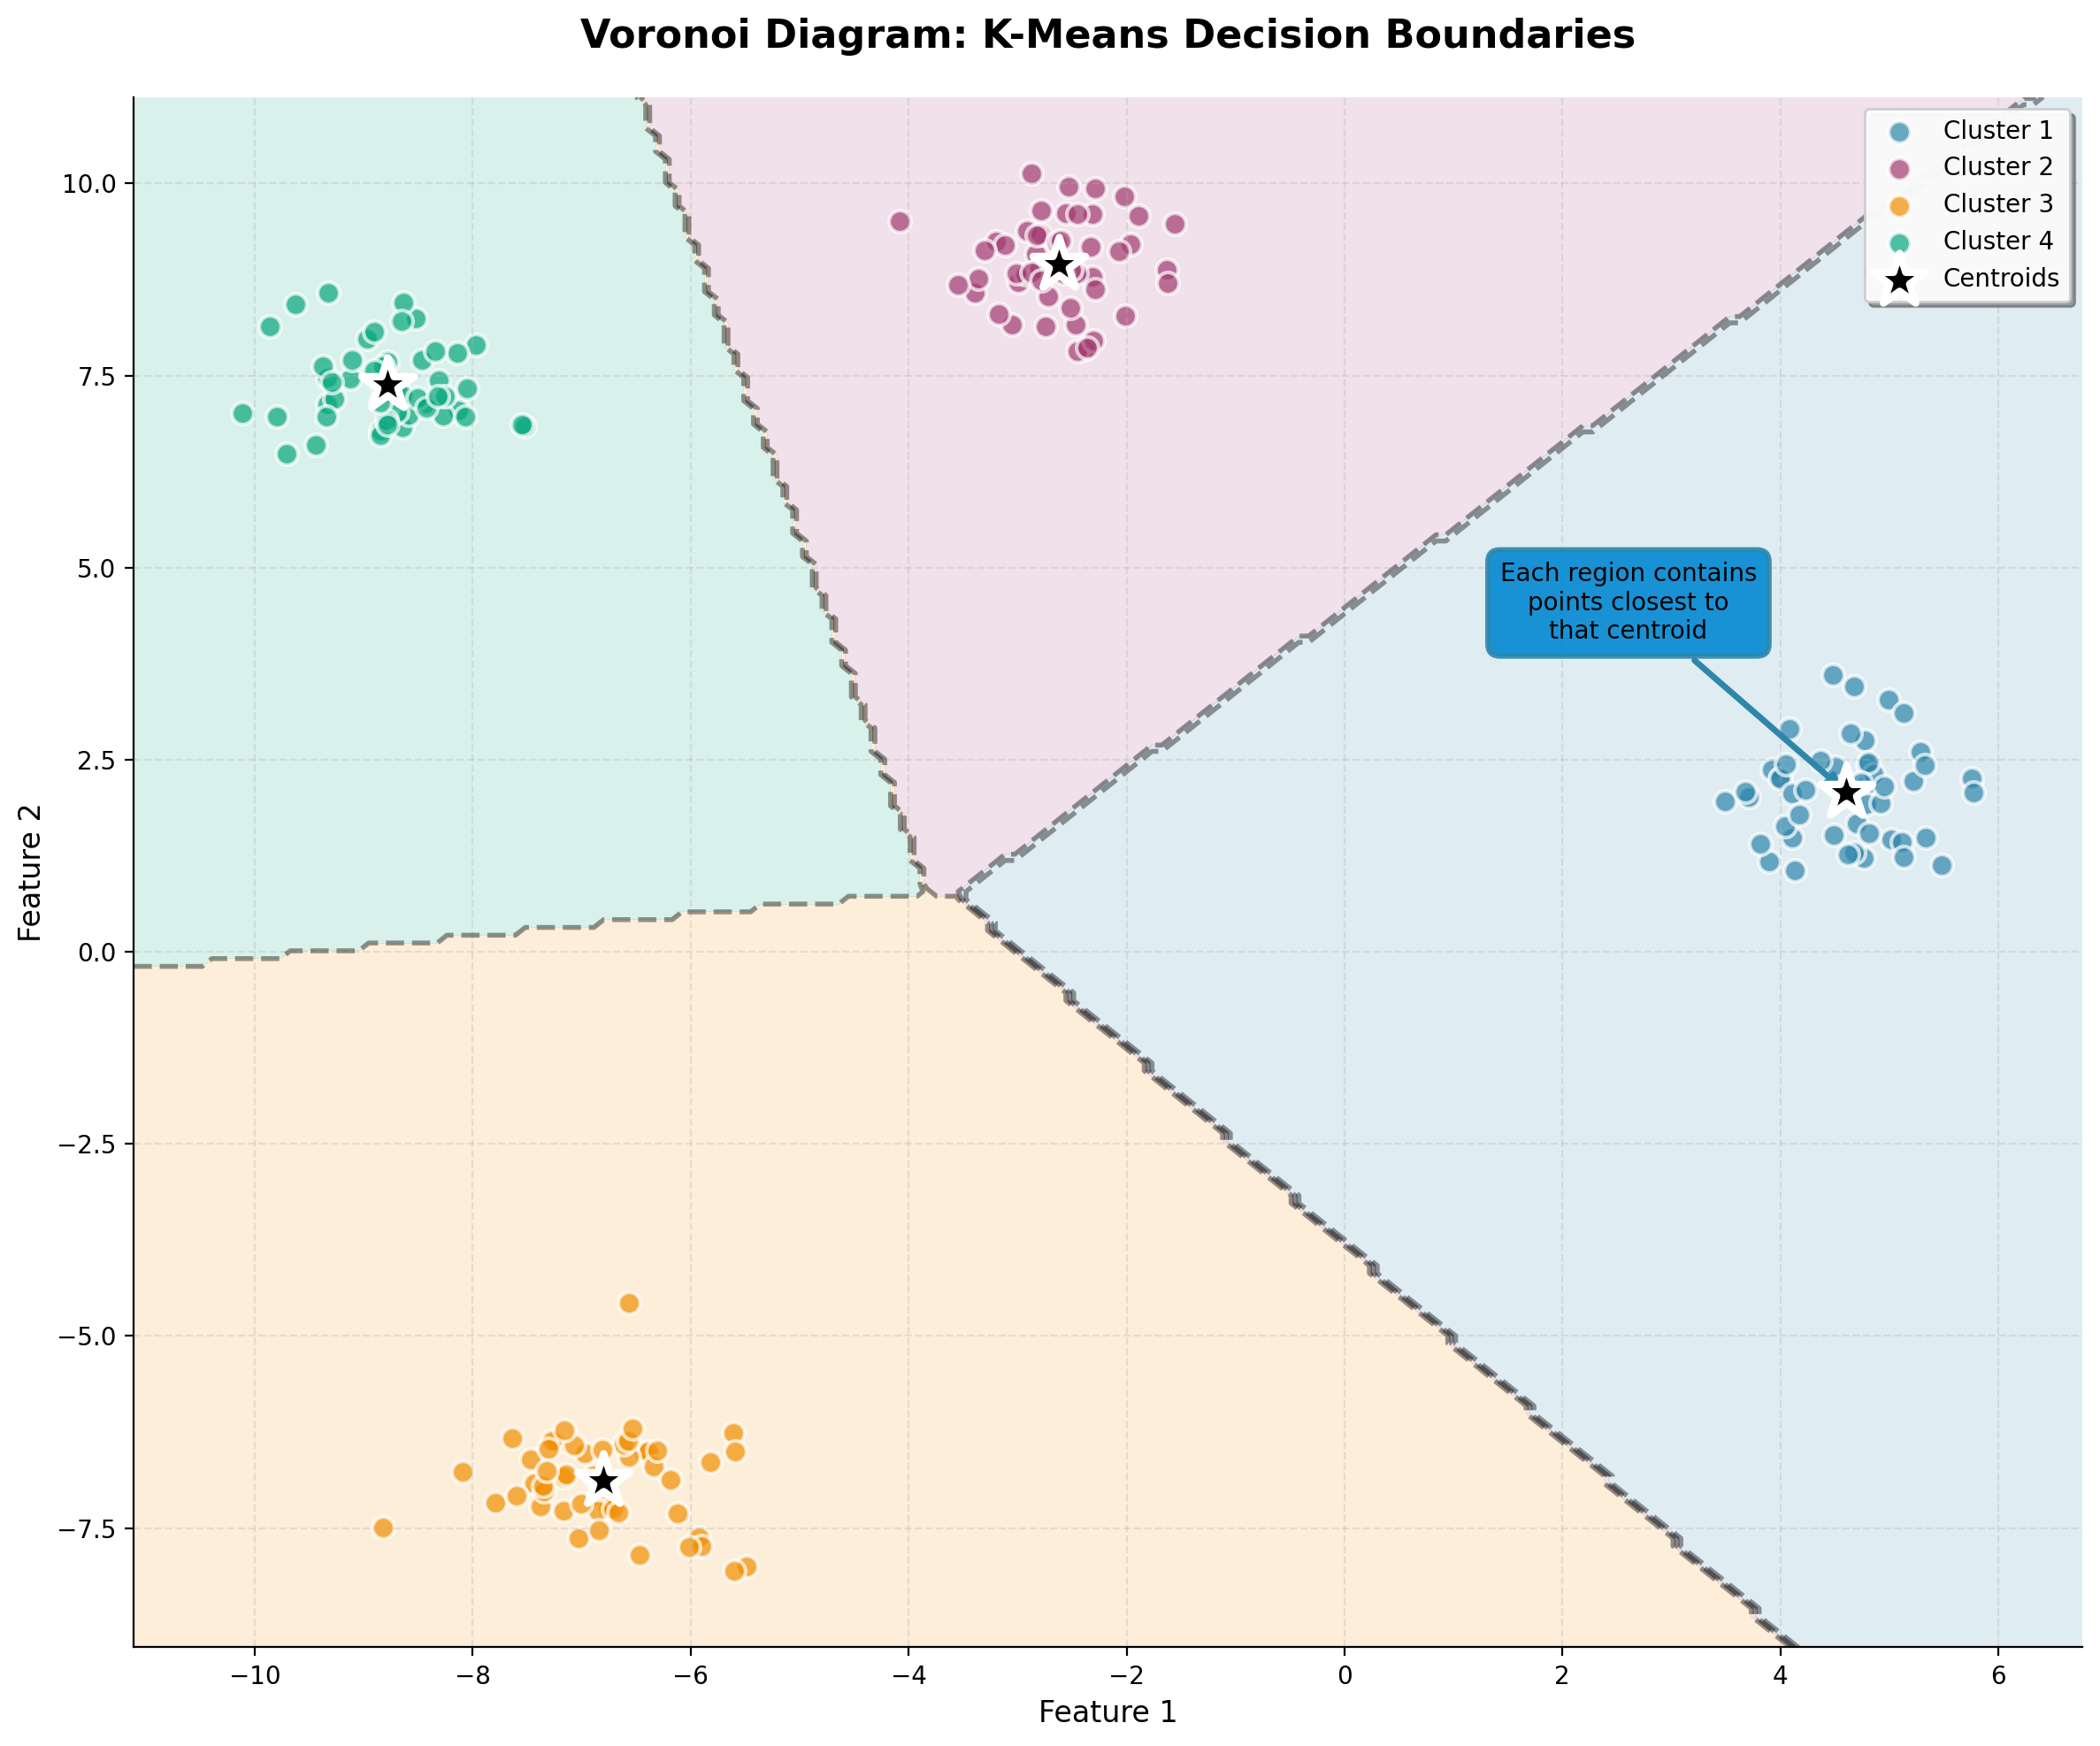
\includegraphics[width=\textwidth]{../figures/voronoi_diagram.png}
\end{column}
\end{columns}
\end{frame}

\begin{frame}{K-Means Initialization: The Challenge}

\centering
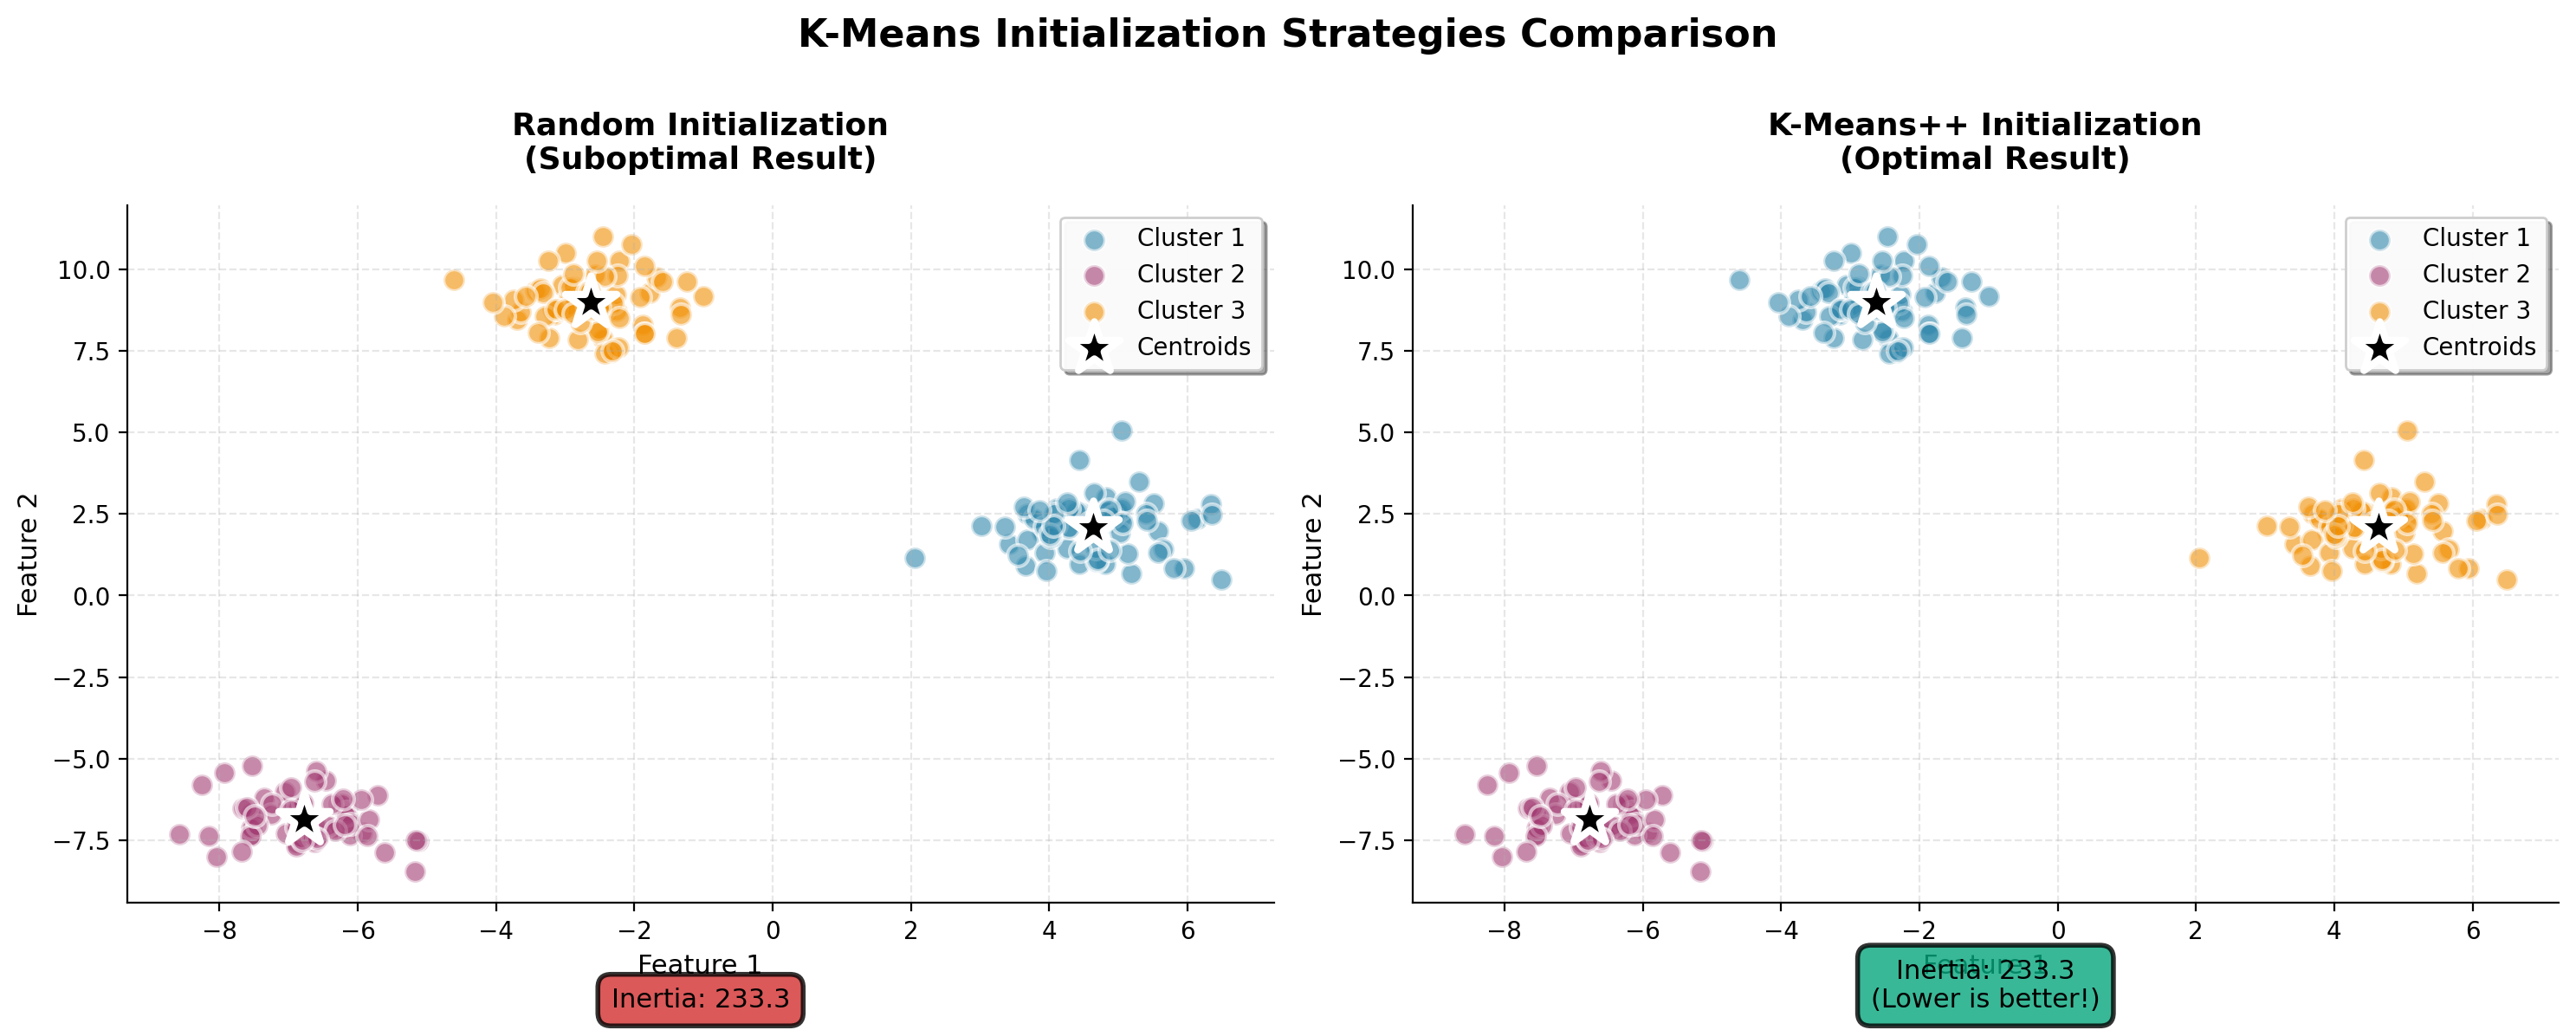
\includegraphics[width=0.88\textwidth]{../figures/kmeans_initialization_comparison.png}

\vspace{0.15cm}

\begin{columns}[T]
\begin{column}{0.32\textwidth}
\begin{alertblock}{Problem}
Sensitive to initial centroids
\end{alertblock}
\end{column}

\begin{column}{0.34\textwidth}
\begin{block}{Random Init Issues}
\begin{itemize}
\setlength{\itemsep}{0pt}
\item Poor local minima
\item High variance
\item Multiple runs needed
\end{itemize}
\end{block}
\end{column}

\begin{column}{0.32\textwidth}
\begin{exampleblock}{Practice}
Run 10-100 times, keep best WCSS
\end{exampleblock}
\end{column}
\end{columns}
\end{frame}

\begin{frame}{K-Means++ Initialization}
\textbf{Smarter initialization strategy (Arthur \& Vassilvitskii, 2007)}

\vspace{0.2cm}

\begin{block}{K-Means++ Algorithm}
\begin{enumerate}
\setlength{\itemsep}{3pt}
\item Choose first centroid $\boldsymbol{\mu}_1$ uniformly at random from data points
\item For $k = 2, \ldots, K$:
\begin{itemize}
\item For each point $\mathbf{x}_i$, compute $D(\mathbf{x}_i)$ = distance to nearest centroid
\item Choose next centroid $\boldsymbol{\mu}_k$ with probability $\propto D(\mathbf{x}_i)^2$
\end{itemize}
\item Run standard K-Means with these initial centroids
\end{enumerate}
\end{block}

\vspace{0.15cm}

\begin{exampleblock}{Advantages}
\begin{itemize}
\setlength{\itemsep}{2pt}
\item Spreads out initial centroids
\item Provably better: $O(\log K)$-competitive with optimal
\item Lower variance, more consistent results
\item Standard in scikit-learn and most libraries
\end{itemize}
\end{exampleblock}

\vspace{0.05cm}

\begin{alertblock}{Recommendation}
\textbf{Always use K-Means++} unless you have domain knowledge for better initialization.
\end{alertblock}
\end{frame}

\begin{frame}{Choosing K: The Elbow Method}

\begin{columns}[T]
\begin{column}{0.58\textwidth}
\begin{block}{Elbow Method}
\begin{enumerate}
\setlength{\itemsep}{1pt}
\item Run K-Means for $K = 1, 2, \ldots, K_{\max}$
\item Plot WCSS vs $K$
\item Look for the "\textbf{elbow}" point
\item Choose $K$ with diminishing returns
\end{enumerate}
\end{block}

\begin{exampleblock}{Interpretation}
\begin{itemize}
\setlength{\itemsep}{1pt}
\item WCSS decreases as $K$ increases
\item Elbow = fit vs complexity trade-off
\item Not always clear/unique
\end{itemize}
\end{exampleblock}
\end{column}

\begin{column}{0.40\textwidth}
\centering
\vspace{0pt}
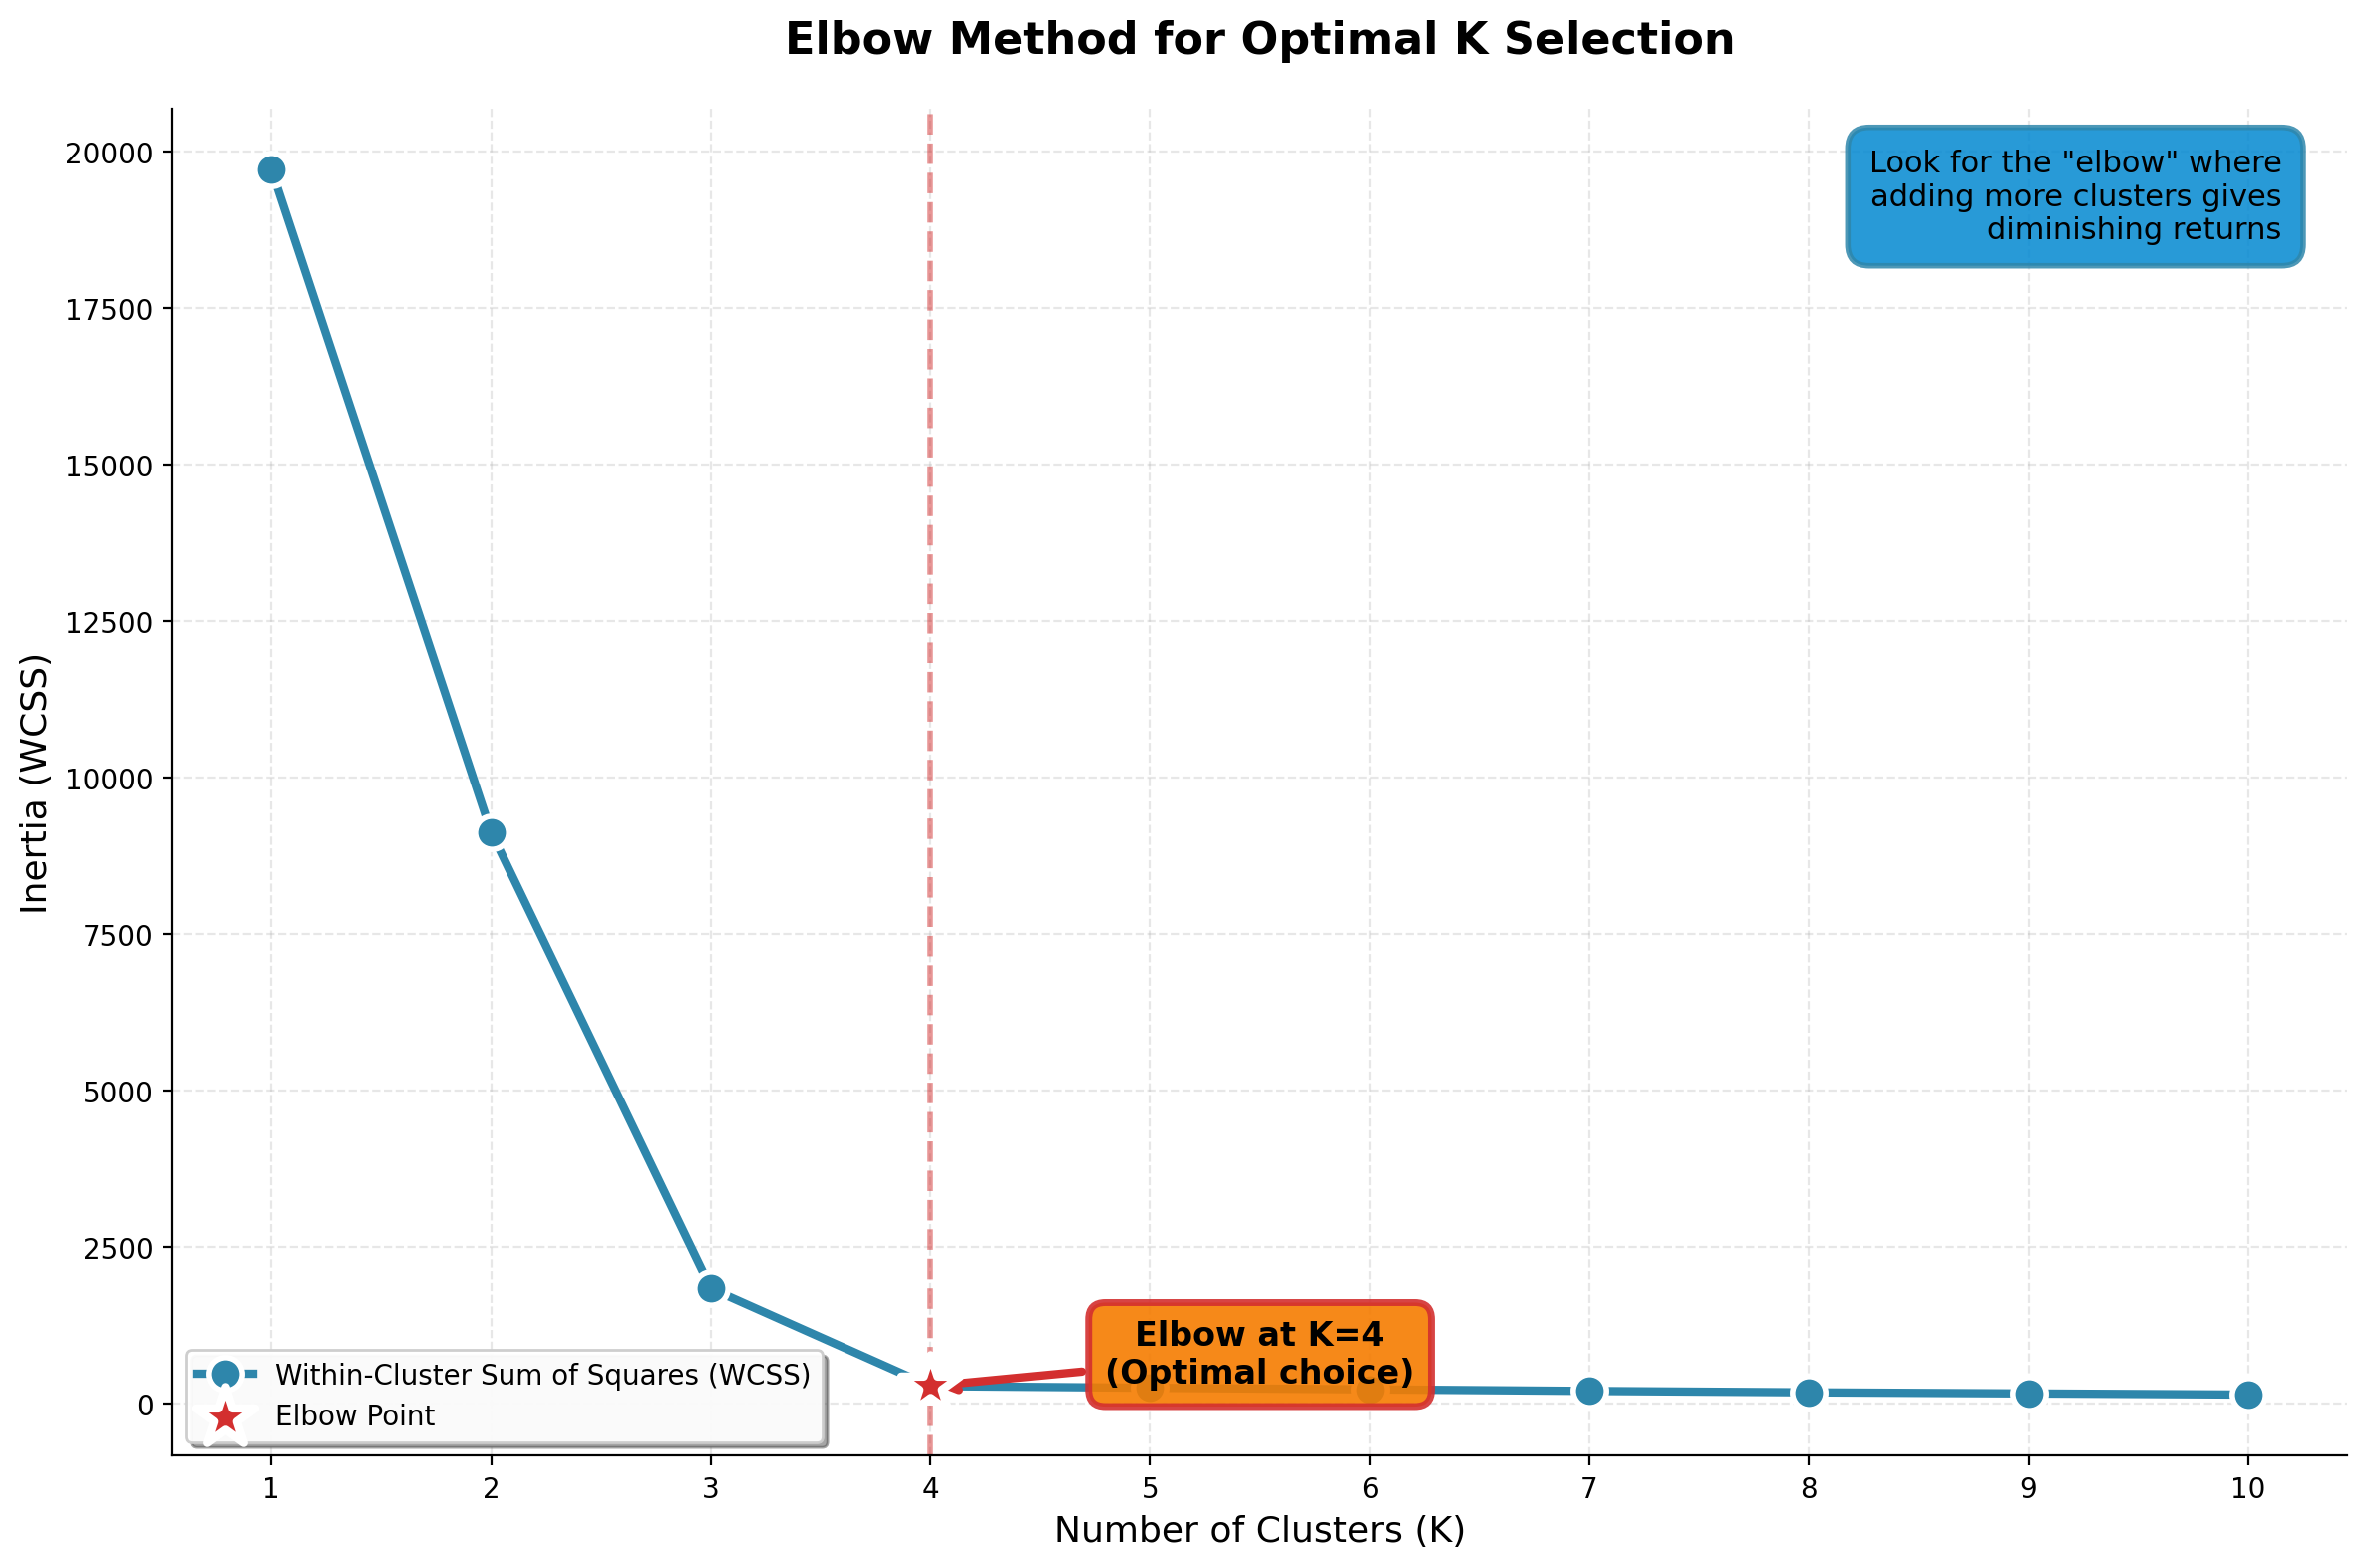
\includegraphics[width=\textwidth]{../figures/elbow_method.png}
\end{column}
\end{columns}
\end{frame}

\begin{frame}{Choosing K: Silhouette Analysis}

\begin{columns}[T]
\begin{column}{0.58\textwidth}
\begin{block}{Silhouette Coefficient}
For each point $\mathbf{x}_i$:

\textbf{1.} $a_i$ = avg distance to same cluster

\textbf{2.} $b_i$ = avg distance to nearest other

\textbf{3.} Silhouette:
$$s_i = \frac{b_i - a_i}{\max(a_i, b_i)}$$

\textbf{Range:} $s_i \in [-1, 1]$
\begin{itemize}
\setlength{\itemsep}{0pt}
\item $s_i \approx 1$: Well clustered
\item $s_i \approx 0$: On border
\item $s_i < 0$: Wrong cluster
\end{itemize}
\end{block}

\begin{alertblock}{Usage}
Choose $K$ maximizing avg score
\end{alertblock}
\end{column}

\begin{column}{0.40\textwidth}
\centering
\vspace{0pt}
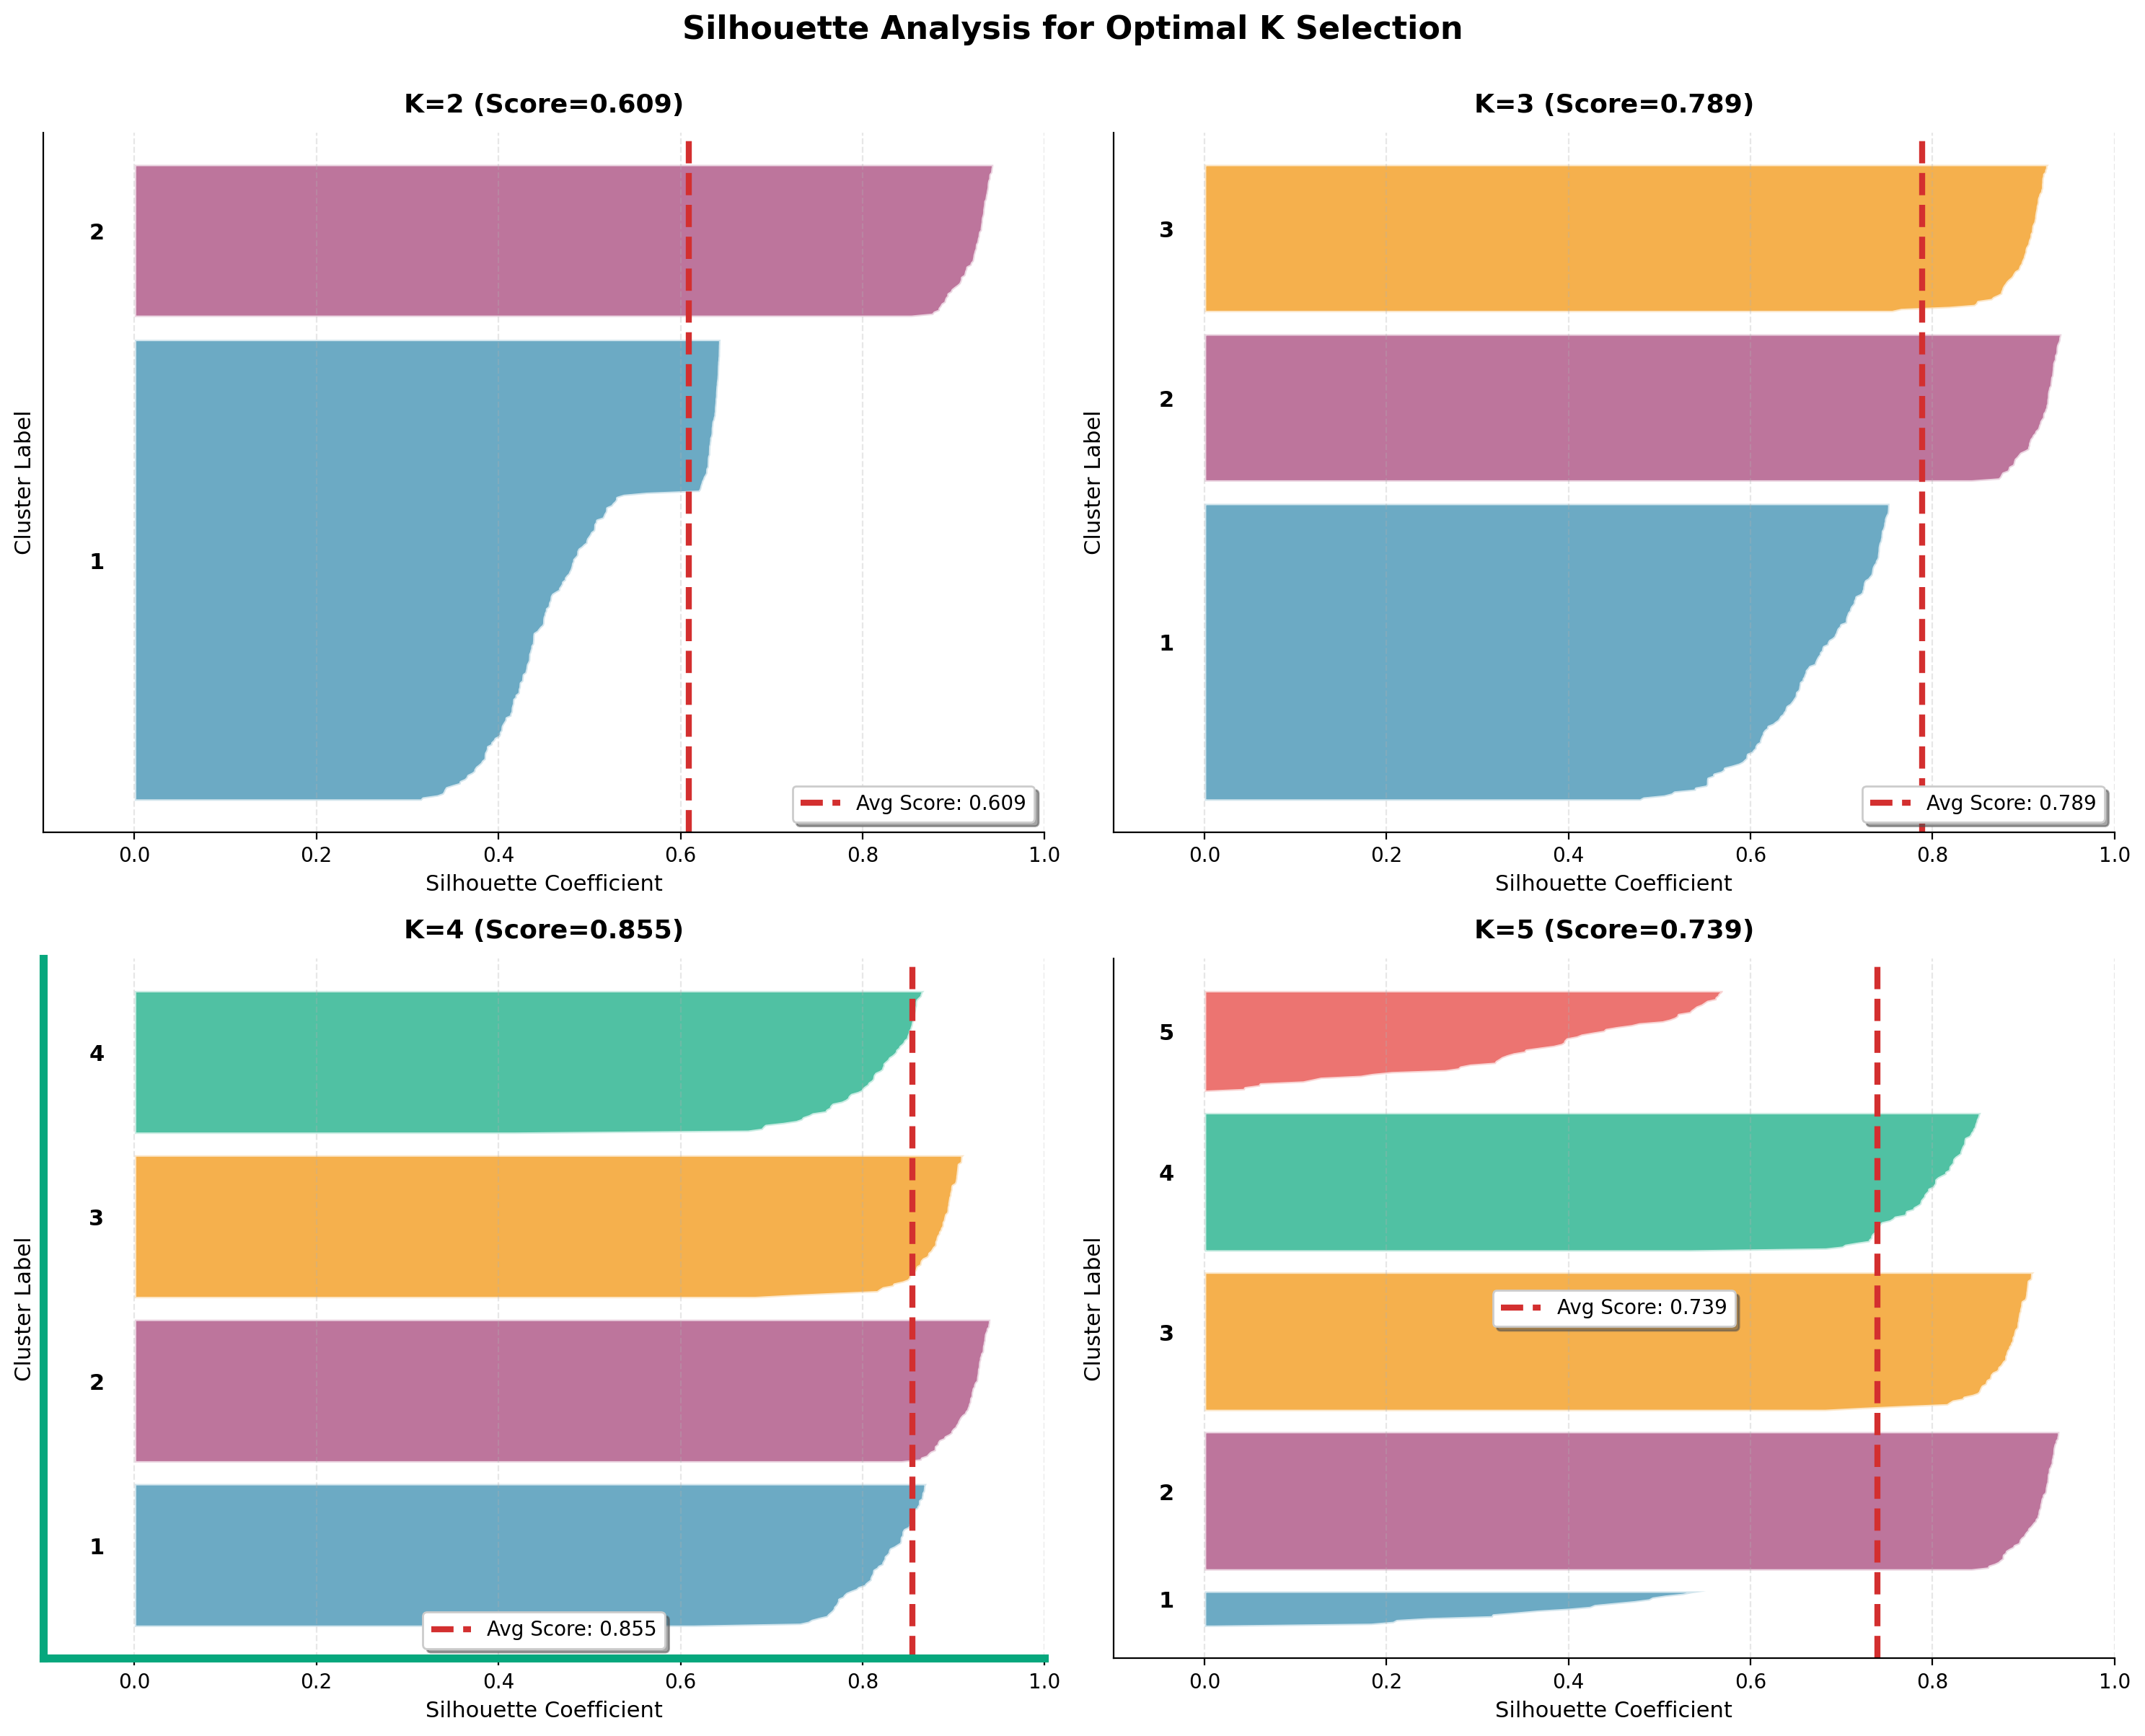
\includegraphics[width=\textwidth]{../figures/silhouette_analysis.png}
\end{column}
\end{columns}
\end{frame}

% ========================================
% Section: Gaussian Mixture Models
% ========================================

\section{Soft Clustering: Gaussian Mixture Models}

\begin{frame}{Limitations of K-Means}

\centering
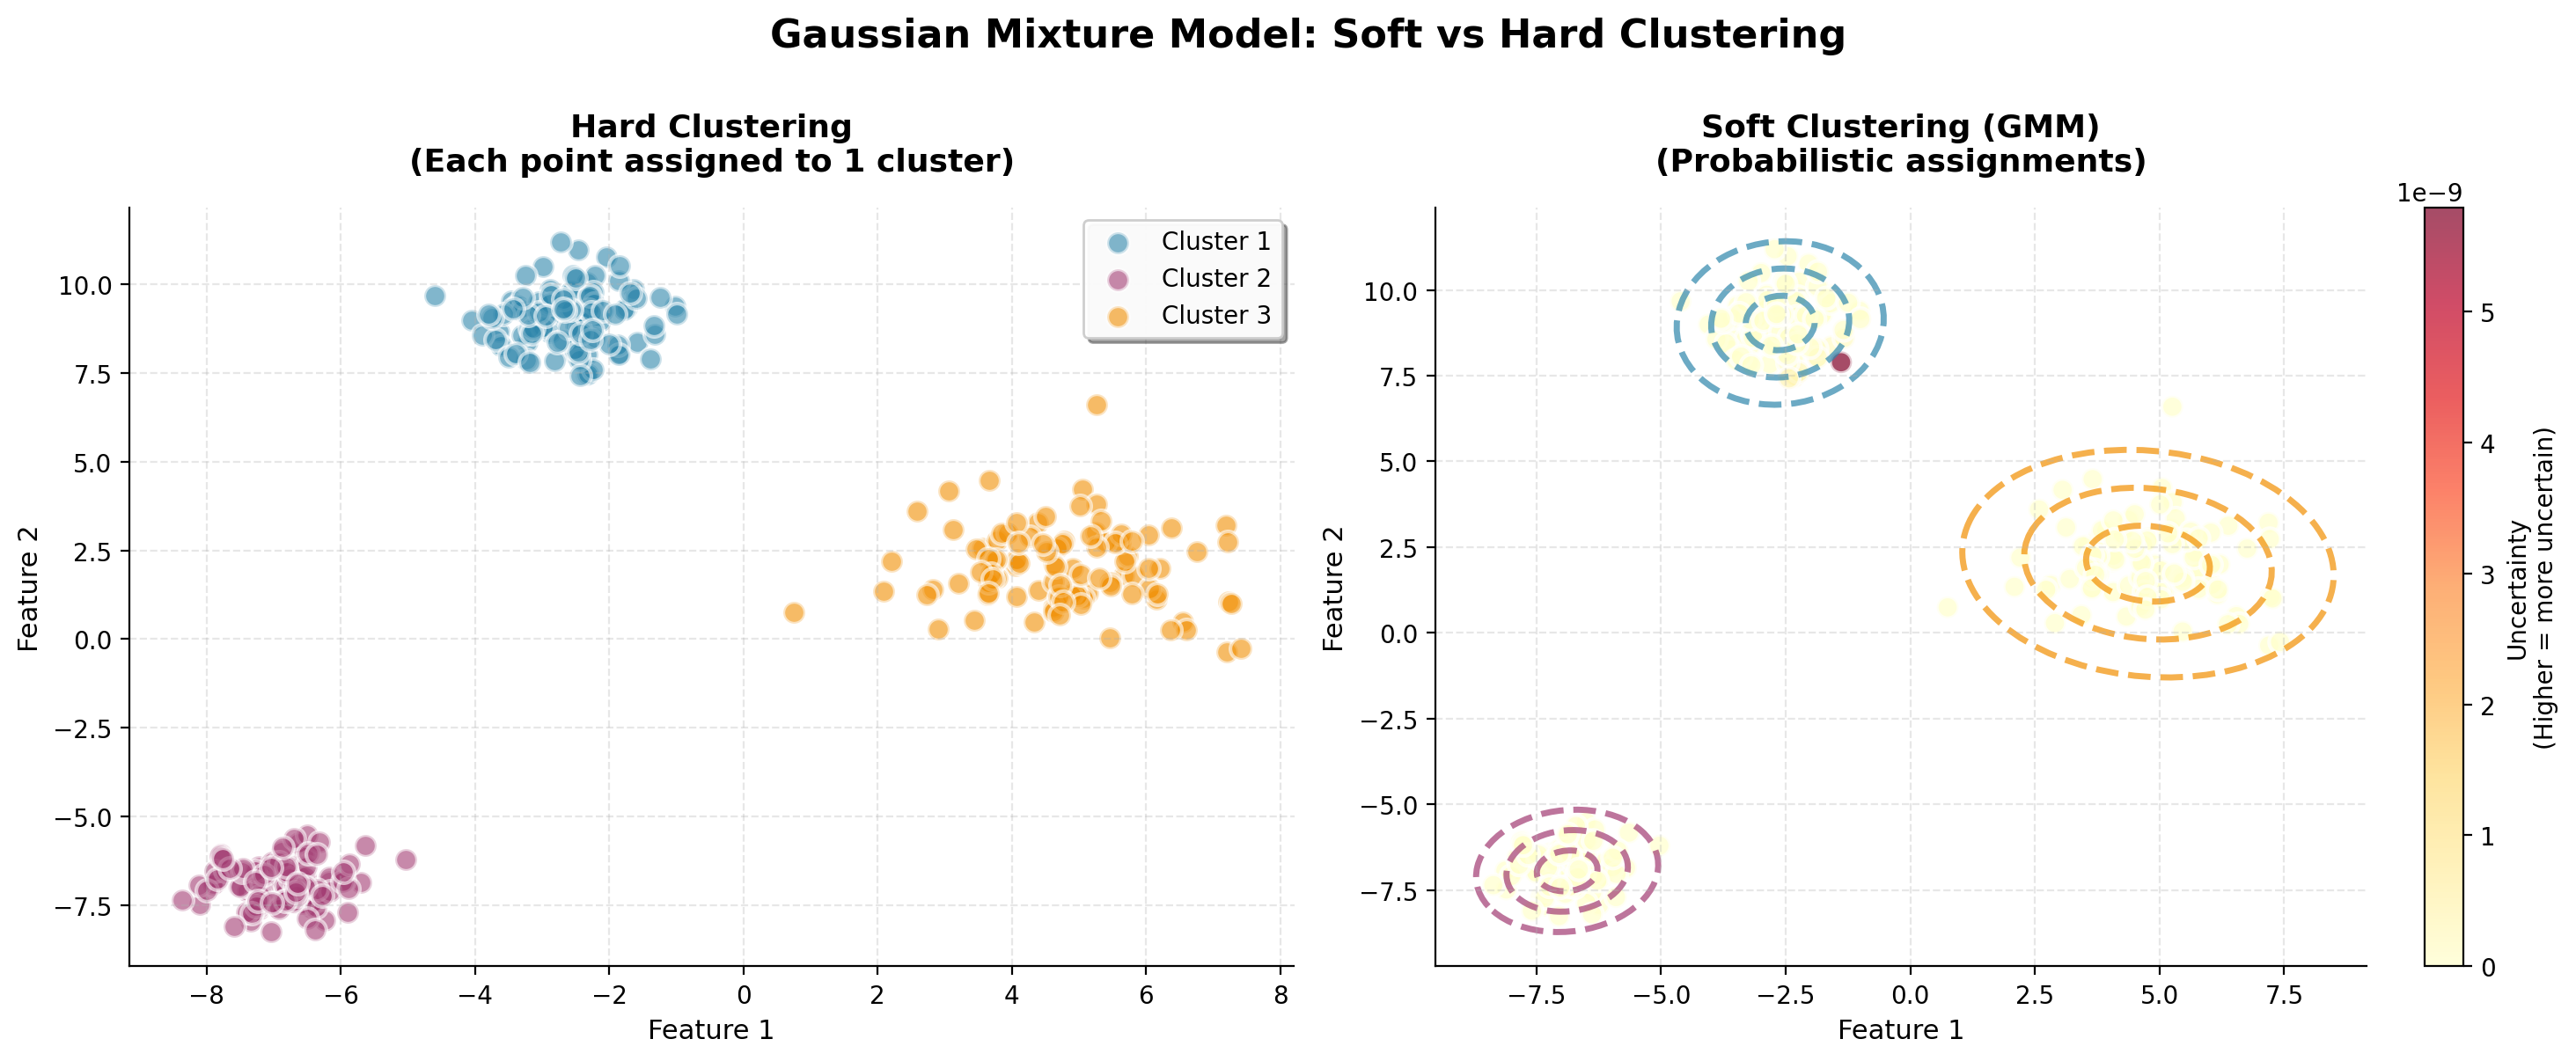
\includegraphics[width=0.78\textwidth]{../figures/gmm_soft_clustering.png}

\vspace{0.15cm}

\begin{columns}[T]
\begin{column}{0.48\textwidth}
\begin{alertblock}{Key Issues}
\begin{itemize}
\setlength{\itemsep}{1pt}
\item \textbf{Hard assignments}: Binary membership
\item \textbf{Spherical clusters}: Equal variance assumed
\item \textbf{No uncertainty}: Can't express doubt
\item \textbf{Outliers}: Forced into clusters
\end{itemize}
\end{alertblock}
\end{column}

\begin{column}{0.48\textwidth}
\begin{exampleblock}{When K-Means Struggles}
\begin{itemize}
\setlength{\itemsep}{1pt}
\item Elongated/elliptical clusters
\item Different sizes/densities
\item Overlapping clusters
\item Need probability of membership
\end{itemize}
\end{exampleblock}
\end{column}
\end{columns}

\vspace{0.08cm}

\begin{tipblock}{Solution}
\textbf{Gaussian Mixture Models (GMM)} provide soft, probabilistic clustering
\end{tipblock}
\end{frame}

\begin{frame}{Gaussian Mixture Models: Formulation}
\textbf{Model data as generated from mixture of $K$ Gaussian distributions}

\vspace{0.2cm}

\begin{block}{Generative Model}
$$p(\mathbf{x}) = \sum_{k=1}^{K} \pi_k \mathcal{N}(\mathbf{x} | \boldsymbol{\mu}_k, \boldsymbol{\Sigma}_k)$$

where:
\begin{itemize}
\item $\pi_k$ = mixing coefficient (prior probability of cluster $k$), $\sum_k \pi_k = 1$
\item $\boldsymbol{\mu}_k$ = mean of Gaussian $k$
\item $\boldsymbol{\Sigma}_k$ = covariance matrix of Gaussian $k$
\item $\mathcal{N}(\mathbf{x} | \boldsymbol{\mu}, \boldsymbol{\Sigma})$ = multivariate Gaussian
\end{itemize}
\end{block}

\vspace{0.15cm}

\begin{exampleblock}{Soft Assignment}
Probability that point $\mathbf{x}_i$ belongs to cluster $k$:
$$\gamma_{ik} = p(z_i = k | \mathbf{x}_i) = \frac{\pi_k \mathcal{N}(\mathbf{x}_i | \boldsymbol{\mu}_k, \boldsymbol{\Sigma}_k)}{\sum_{j=1}^{K} \pi_j \mathcal{N}(\mathbf{x}_i | \boldsymbol{\mu}_j, \boldsymbol{\Sigma}_j)}$$
\end{exampleblock}
\end{frame}

\begin{frame}{GMM: Expectation-Maximization Algorithm}
\textbf{Learn parameters $\{\pi_k, \boldsymbol{\mu}_k, \boldsymbol{\Sigma}_k\}$ using EM}

\vspace{0.2cm}

\begin{block}{EM Algorithm}
\textbf{Initialize:} Random $\boldsymbol{\mu}_k$, $\boldsymbol{\Sigma}_k = I$, $\pi_k = 1/K$

\vspace{0.1cm}

\textbf{Repeat until convergence:}

\vspace{0.1cm}

\textbf{E-step:} Compute responsibilities (soft assignments)
$$\gamma_{ik} = \frac{\pi_k \mathcal{N}(\mathbf{x}_i | \boldsymbol{\mu}_k, \boldsymbol{\Sigma}_k)}{\sum_{j=1}^{K} \pi_j \mathcal{N}(\mathbf{x}_i | \boldsymbol{\mu}_j, \boldsymbol{\Sigma}_j)}$$

\textbf{M-step:} Update parameters
$$\pi_k = \frac{1}{n}\sum_{i=1}^{n} \gamma_{ik}, \quad
\boldsymbol{\mu}_k = \frac{\sum_i \gamma_{ik} \mathbf{x}_i}{\sum_i \gamma_{ik}}, \quad
\boldsymbol{\Sigma}_k = \frac{\sum_i \gamma_{ik} (\mathbf{x}_i - \boldsymbol{\mu}_k)(\mathbf{x}_i - \boldsymbol{\mu}_k)^T}{\sum_i \gamma_{ik}}$$
\end{block}

\vspace{0.1cm}

\begin{alertblock}{Properties}
Monotonically increases likelihood. Guaranteed to converge to local maximum.
\end{alertblock}
\end{frame}

\begin{frame}{GMM vs K-Means Comparison}
\begin{columns}[t]
\begin{column}{0.48\textwidth}
\begin{block}{K-Means}
\textbf{Pros:}
\begin{itemize}
\setlength{\itemsep}{2pt}
\item Simple, fast, scalable
\item Easy to implement
\item Works well for spherical clusters
\item Less parameters to tune
\end{itemize}

\vspace{0.1cm}

\textbf{Cons:}
\begin{itemize}
\setlength{\itemsep}{2pt}
\item Hard assignments only
\item Assumes spherical clusters
\item Sensitive to initialization
\item No measure of uncertainty
\end{itemize}
\end{block}
\end{column}

\begin{column}{0.48\textwidth}
\begin{block}{GMM}
\textbf{Pros:}
\begin{itemize}
\setlength{\itemsep}{2pt}
\item Soft probabilistic assignments
\item Flexible cluster shapes (elliptical)
\item Measures uncertainty
\item Principled statistical model
\end{itemize}

\vspace{0.1cm}

\textbf{Cons:}
\begin{itemize}
\setlength{\itemsep}{2pt}
\item Slower than K-Means
\item More parameters ($\boldsymbol{\Sigma}_k$)
\item Can overfit with full covariance
\item Also sensitive to initialization
\end{itemize}
\end{block}
\end{column}
\end{columns}

\vspace{0.1cm}

\begin{alertblock}{Note}
K-Means is special case of GMM with $\boldsymbol{\Sigma}_k = \sigma^2 I$ and hard assignments!
\end{alertblock}
\end{frame}

% ========================================
% Section: Hierarchical Clustering
% ========================================

\section{Hierarchical Clustering}

\begin{frame}{Hierarchical Clustering: Overview}

\centering
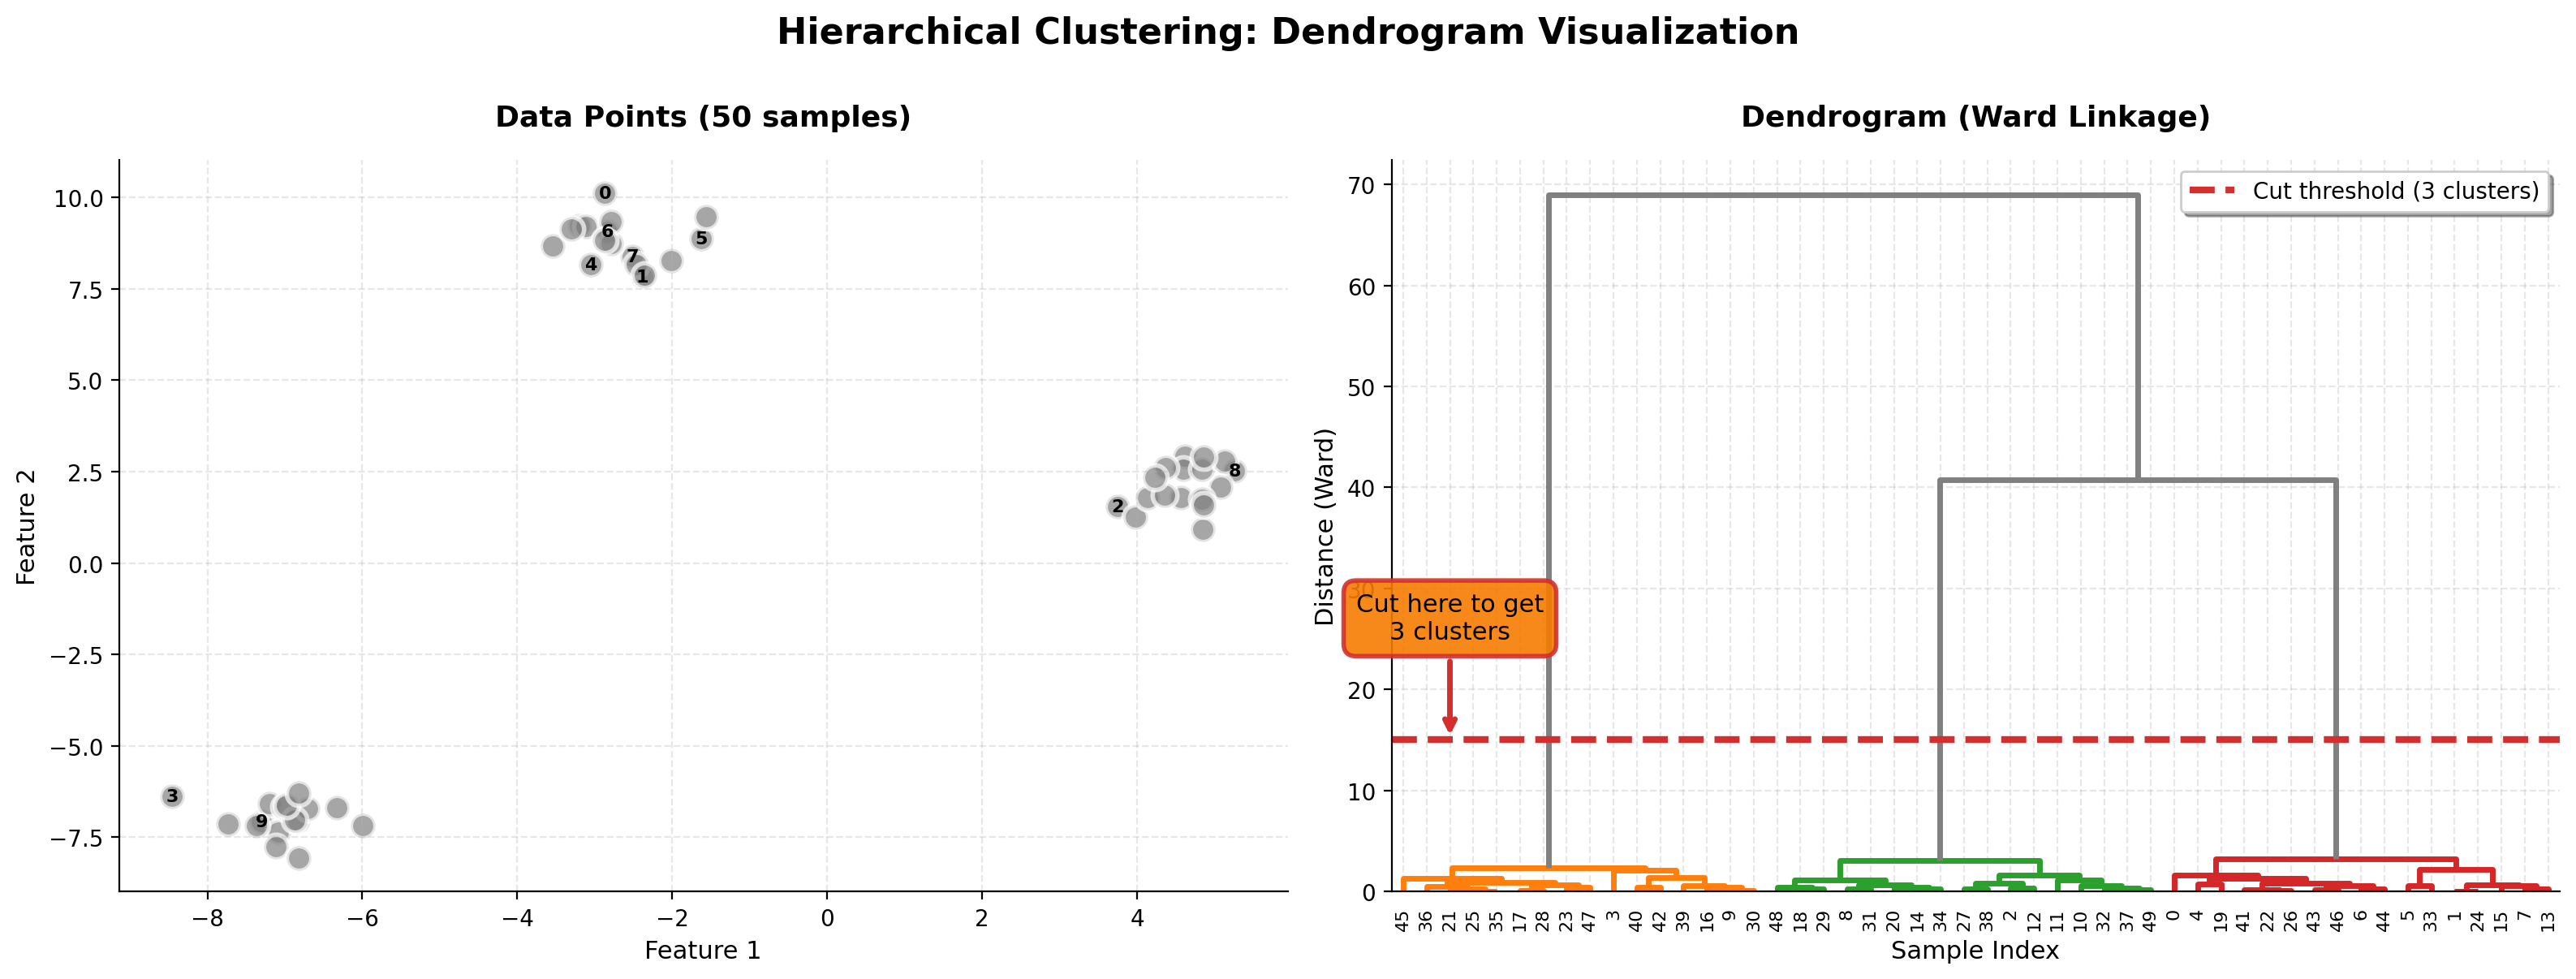
\includegraphics[width=0.72\textwidth]{../figures/hierarchical_dendrogram.png}

\vspace{0.15cm}

\begin{columns}[T]
\begin{column}{0.48\textwidth}
\begin{block}{Agglomerative (Bottom-up)}
\begin{itemize}
\setlength{\itemsep}{1pt}
\item Start: Each point = cluster
\item Merge closest clusters
\item End: One cluster
\end{itemize}
\end{block}
\end{column}

\begin{column}{0.48\textwidth}
\begin{block}{Divisive (Top-down)}
\begin{itemize}
\setlength{\itemsep}{1pt}
\item Start: All in one cluster
\item Split clusters iteratively
\item End: Each point separate
\end{itemize}
\end{block}
\end{column}
\end{columns}

\vspace{0.08cm}

\begin{exampleblock}{Key Advantage}
No need to specify $K$ upfront! Cut dendrogram at any height to get desired clusters.
\end{exampleblock}
\end{frame}

\begin{frame}{Agglomerative Clustering Algorithm}
\textbf{Most common hierarchical method}

\vspace{0.2cm}

\begin{block}{Algorithm}
\begin{enumerate}
\setlength{\itemsep}{3pt}
\item \textbf{Initialize}: Each of $n$ points is own cluster
\item \textbf{Compute}: Distance matrix between all clusters
\item \textbf{Repeat} until one cluster remains:
\begin{itemize}
\item Find pair of closest clusters
\item Merge them into single cluster
\item Update distance matrix
\end{itemize}
\item \textbf{Output}: Dendrogram showing merge history
\end{enumerate}
\end{block}

\vspace{0.15cm}

\begin{exampleblock}{Complexity}
\textbf{Time:} $O(n^2 \log n)$ with efficient data structures

\textbf{Space:} $O(n^2)$ for distance matrix
\end{exampleblock}

\vspace{0.05cm}

\begin{alertblock}{Challenge}
How do we measure distance between \textbf{clusters} (not just points)?
\end{alertblock}
\end{frame}

% ========================================
% Hierarchical Clustering Step-by-Step Example
% ========================================

\begin{frame}{Hierarchical Clustering Example: Dataset}
\textbf{Let's apply Agglomerative Clustering to 5 points (Single Linkage)}

\vspace{0.15cm}

\begin{columns}[T]
\begin{column}{0.38\textwidth}
\begin{block}{Dataset (5 points, 1D)}
\begin{center}
\begin{tabular}{cc}
\toprule
Point & Position \\
\midrule
A & 2 \\
B & 4 \\
C & 5 \\
D & 10 \\
E & 12 \\
\bottomrule
\end{tabular}
\end{center}
\end{block}

\vspace{0.1cm}

\begin{exampleblock}{Goal}
Build dendrogram using \textbf{Single Linkage}
\end{exampleblock}
\end{column}

\begin{column}{0.60\textwidth}
\centering
\begin{tikzpicture}[scale=1.1]
% Number line
\draw[-stealth] (0,0) -- (14,0) node[right] {$x$};

% Tick marks
\draw (0,0.1) -- (0,-0.1) node[below] {\tiny 0};
\draw (2,0.1) -- (2,-0.1) node[below] {\tiny 2};
\draw (4,0.1) -- (4,-0.1) node[below] {\tiny 4};
\draw (6,0.1) -- (6,-0.1) node[below] {\tiny 6};
\draw (8,0.1) -- (8,-0.1) node[below] {\tiny 8};
\draw (10,0.1) -- (10,-0.1) node[below] {\tiny 10};
\draw (12,0.1) -- (12,-0.1) node[below] {\tiny 12};

% Data points
\fill[blue] (2,0) circle (2.5pt) node[above=3pt] {A};
\fill[blue] (4,0) circle (2.5pt) node[above=3pt] {B};
\fill[blue] (5,0) circle (2.5pt) node[above=3pt] {C};
\fill[blue] (10,0) circle (2.5pt) node[above=3pt] {D};
\fill[blue] (12,0) circle (2.5pt) node[above=3pt] {E};
\end{tikzpicture}

\vspace{0.3cm}

\begin{alertblock}{Initial State}
Each point = own cluster\\
5 clusters: \{A\}, \{B\}, \{C\}, \{D\}, \{E\}
\end{alertblock}
\end{column}
\end{columns}
\end{frame}

\begin{frame}{Hierarchical Example: Step 1 - Distance Matrix}
\textbf{Step 1: Compute pairwise distance matrix}

\vspace{0.15cm}

\begin{columns}[T]
\begin{column}{0.48\textwidth}
\begin{block}{Distance Matrix}
\small
\begin{center}
\begin{tabular}{c|ccccc}
 & A & B & C & D & E \\
\hline
A & 0 & \textcolor{red}{\textbf{2}} & 3 & 8 & 10 \\
B & \textcolor{red}{\textbf{2}} & 0 & \textcolor{blue}{\textbf{1}} & 6 & 8 \\
C & 3 & \textcolor{blue}{\textbf{1}} & 0 & 5 & 7 \\
D & 8 & 6 & 5 & 0 & \textcolor{green!60!black}{\textbf{2}} \\
E & 10 & 8 & 7 & \textcolor{green!60!black}{\textbf{2}} & 0 \\
\end{tabular}
\end{center}
\end{block}

\vspace{0.1cm}

\begin{exampleblock}{Find Minimum}
Smallest distance = \textbf{1} between B and C

$\Rightarrow$ Merge \{B\} and \{C\}
\end{exampleblock}
\end{column}

\begin{column}{0.50\textwidth}
\centering
\textbf{Dendrogram (Step 1)}

\vspace{0.15cm}

\begin{tikzpicture}[scale=0.9]
% Leaves
\node (A) at (0,0) {A};
\node (B) at (2,0) {B};
\node (C) at (3,0) {C};
\node (D) at (5,0) {D};
\node (E) at (6,0) {E};

% First merge: B-C at height 1
\draw (B) -- (2.5,1);
\draw (C) -- (2.5,1);
\draw[blue, line width=1.5pt] (2.5,1) -- (2.5,1.5) node[right, black] {\tiny h=1};

% Y-axis
\draw[-stealth] (-0.5,0) -- (-0.5,5) node[above] {\tiny height};
\draw (-0.6,0) -- (-0.4,0) node[left] {\tiny 0};
\draw (-0.6,1) -- (-0.4,1) node[left] {\tiny 1};
\draw (-0.6,2) -- (-0.4,2) node[left] {\tiny 2};
\draw (-0.6,3) -- (-0.4,3) node[left] {\tiny 3};
\draw (-0.6,4) -- (-0.4,4) node[left] {\tiny 4};
\draw (-0.6,5) -- (-0.4,5) node[left] {\tiny 5};
\end{tikzpicture}

\vspace{0.2cm}

\begin{alertblock}{Current Clusters}
\{A\}, \{\textcolor{blue}{B, C}\}, \{D\}, \{E\}\\
4 clusters remain
\end{alertblock}
\end{column}
\end{columns}
\end{frame}

\begin{frame}{Hierarchical Example: Step 2 - Update Matrix}
\textbf{Step 2: Update distance matrix using Single Linkage}

\vspace{0.15cm}

\begin{columns}[T]
\begin{column}{0.48\textwidth}
\begin{block}{Single Linkage Rule}
$$d(\{B,C\}, X) = \min(d(B,X), d(C,X))$$

\vspace{0.1cm}

New distances to cluster \{B,C\}:
\begin{itemize}
\setlength{\itemsep}{2pt}
\item $d(\{B,C\}, A) = \min(2, 3) = \mathbf{2}$
\item $d(\{B,C\}, D) = \min(6, 5) = \mathbf{5}$
\item $d(\{B,C\}, E) = \min(8, 7) = \mathbf{7}$
\end{itemize}
\end{block}

\vspace{0.1cm}

\begin{block}{Updated Matrix}
\small
\begin{center}
\begin{tabular}{c|cccc}
 & A & \{B,C\} & D & E \\
\hline
A & 0 & \textcolor{red}{\textbf{2}} & 8 & 10 \\
\{B,C\} & \textcolor{red}{\textbf{2}} & 0 & 5 & 7 \\
D & 8 & 5 & 0 & \textcolor{green!60!black}{\textbf{2}} \\
E & 10 & 7 & \textcolor{green!60!black}{\textbf{2}} & 0 \\
\end{tabular}
\end{center}
\end{block}
\end{column}

\begin{column}{0.50\textwidth}
\centering
\textbf{Dendrogram (Step 2)}

\vspace{0.15cm}

\begin{tikzpicture}[scale=0.9]
% Leaves
\node (A) at (0,0) {A};
\node (B) at (2,0) {B};
\node (C) at (3,0) {C};
\node (D) at (5,0) {D};
\node (E) at (6,0) {E};

% First merge: B-C at height 1
\draw (B) -- (2.5,1);
\draw (C) -- (2.5,1);
\draw[blue, line width=1.5pt] (2.5,1) -- (2.5,1.5);

% Second merge: D-E at height 2
\draw (D) -- (5.5,2);
\draw (E) -- (5.5,2);
\draw[green!60!black, line width=1.5pt] (5.5,2) -- (5.5,2.5) node[right, black] {\tiny h=2};

% Y-axis
\draw[-stealth] (-0.5,0) -- (-0.5,5) node[above] {\tiny height};
\draw (-0.6,0) -- (-0.4,0) node[left] {\tiny 0};
\draw (-0.6,1) -- (-0.4,1) node[left] {\tiny 1};
\draw (-0.6,2) -- (-0.4,2) node[left] {\tiny 2};
\draw (-0.6,3) -- (-0.4,3) node[left] {\tiny 3};
\draw (-0.6,4) -- (-0.4,4) node[left] {\tiny 4};
\draw (-0.6,5) -- (-0.4,5) node[left] {\tiny 5};
\end{tikzpicture}

\vspace{0.2cm}

\begin{exampleblock}{Next Merge}
Min distance = \textbf{2}\\
Merge \{D\} and \{E\} at height 2
\end{exampleblock}
\end{column}
\end{columns}
\end{frame}

\begin{frame}{Hierarchical Example: Steps 3-4}
\textbf{Continue merging until one cluster remains}

\vspace{0.15cm}

\begin{columns}[T]
\begin{column}{0.48\textwidth}
\begin{block}{Step 3}
Clusters: \{A\}, \{B,C\}, \{D,E\}

\vspace{0.05cm}

Updated distances:
\begin{itemize}
\setlength{\itemsep}{1pt}
\item $d(A, \{B,C\}) = 2$
\item $d(A, \{D,E\}) = 8$
\item $d(\{B,C\}, \{D,E\}) = 5$
\end{itemize}

\vspace{0.05cm}

\textbf{Min = 2:} Merge A with \{B,C\}\\
New cluster: \{\textcolor{red}{A, B, C}\} at height 2
\end{block}

\vspace{0.1cm}

\begin{block}{Step 4 (Final)}
Clusters: \{A,B,C\}, \{D,E\}

\vspace{0.05cm}

Distance: $d(\{A,B,C\}, \{D,E\}) = 5$

\vspace{0.05cm}

\textbf{Final merge} at height 5\\
One cluster: \{A, B, C, D, E\}
\end{block}
\end{column}

\begin{column}{0.50\textwidth}
\centering
\textbf{Complete Dendrogram}

\vspace{0.15cm}

\begin{tikzpicture}[scale=0.85]
% Leaves
\node (A) at (0,0) {A};
\node (B) at (2,0) {B};
\node (C) at (3,0) {C};
\node (D) at (5,0) {D};
\node (E) at (6,0) {E};

% Merge B-C at h=1
\draw (B) -- (2.5,1);
\draw (C) -- (2.5,1);
\draw[blue, line width=1.2pt] (2.5,1) -- (2.5,2);

% Merge D-E at h=2
\draw (D) -- (5.5,2);
\draw (E) -- (5.5,2);
\draw[green!60!black, line width=1.2pt] (5.5,2) -- (5.5,5);

% Merge A with {B,C} at h=2
\draw (A) -- (0,2) -- (1.25,2);
\draw (2.5,2) -- (1.25,2);
\draw[red, line width=1.2pt] (1.25,2) -- (1.25,5);

% Final merge at h=5
\draw[purple, line width=1.5pt] (1.25,5) -- (3.375,5) -- (5.5,5);

% Height annotations
\node[right] at (3.375,5) {\tiny h=5};
\node[left] at (1.25,2) {\tiny h=2};
\node[left] at (2.5,1) {\tiny h=1};
\node[right] at (5.5,2) {\tiny h=2};

% Y-axis
\draw[-stealth] (-0.8,0) -- (-0.8,5.5) node[above] {\tiny height};
\draw (-0.9,0) -- (-0.7,0) node[left] {\tiny 0};
\draw (-0.9,1) -- (-0.7,1) node[left] {\tiny 1};
\draw (-0.9,2) -- (-0.7,2) node[left] {\tiny 2};
\draw (-0.9,3) -- (-0.7,3) node[left] {\tiny 3};
\draw (-0.9,4) -- (-0.7,4) node[left] {\tiny 4};
\draw (-0.9,5) -- (-0.7,5) node[left] {\tiny 5};
\end{tikzpicture}

\vspace{0.15cm}

\begin{alertblock}{Interpretation}
Cut at different heights to get different K clusters
\end{alertblock}
\end{column}
\end{columns}
\end{frame}

\begin{frame}{Hierarchical Example: Cutting the Dendrogram}
\textbf{Extract different numbers of clusters by cutting at different heights}

\vspace{0.2cm}

\centering
\begin{tikzpicture}[scale=1.0]
% Dendrogram
\node (A) at (0,0) {A};
\node (B) at (2,0) {B};
\node (C) at (3,0) {C};
\node (D) at (5,0) {D};
\node (E) at (6,0) {E};

\draw (B) -- (2.5,1);
\draw (C) -- (2.5,1);
\draw (2.5,1) -- (2.5,2);

\draw (D) -- (5.5,2);
\draw (E) -- (5.5,2);
\draw (5.5,2) -- (5.5,5);

\draw (A) -- (0,2) -- (1.25,2);
\draw (2.5,2) -- (1.25,2);
\draw (1.25,2) -- (1.25,5);

\draw (1.25,5) -- (3.375,5) -- (5.5,5);

% Cut lines
\draw[red, dashed, line width=2pt] (-0.5,4.5) -- (6.5,4.5) node[right] {K=2: \{\textcolor{red}{A,B,C}\}, \{\textcolor{green!60!black}{D,E}\}};
\draw[blue, dashed, line width=2pt] (-0.5,2.5) -- (6.5,2.5) node[right] {K=3: \{\textcolor{red}{A,B,C}\}, \{\textcolor{blue}{D}\}, \{\textcolor{blue}{E}\}};
\draw[orange, dashed, line width=2pt] (-0.5,1.5) -- (6.5,1.5) node[right] {K=4: \{\textcolor{orange}{A}\}, \{\textcolor{orange}{B,C}\}, \{D\}, \{E\}};

% Y-axis
\draw[-stealth] (-0.8,0) -- (-0.8,5.5) node[above] {height};
\draw (-0.9,0) -- (-0.7,0) node[left] {\tiny 0};
\draw (-0.9,1) -- (-0.7,1) node[left] {\tiny 1};
\draw (-0.9,2) -- (-0.7,2) node[left] {\tiny 2};
\draw (-0.9,3) -- (-0.7,3) node[left] {\tiny 3};
\draw (-0.9,4) -- (-0.7,4) node[left] {\tiny 4};
\draw (-0.9,5) -- (-0.7,5) node[left] {\tiny 5};
\end{tikzpicture}

\vspace{0.2cm}

\begin{alertblock}{Key Advantage of Hierarchical Clustering}
No need to pre-specify K! The dendrogram shows the full hierarchy.
\end{alertblock}
\end{frame}

\begin{frame}{Linkage Criteria}
\textbf{Different ways to measure inter-cluster distance}

\vspace{0.2cm}

\begin{block}{Common Linkage Methods}
For clusters $C_i$ and $C_j$:

\vspace{0.1cm}

\textbf{1. Single Linkage (MIN):}
$$d(C_i, C_j) = \min_{\mathbf{x} \in C_i, \mathbf{y} \in C_j} d(\mathbf{x}, \mathbf{y})$$

\textbf{2. Complete Linkage (MAX):}
$$d(C_i, C_j) = \max_{\mathbf{x} \in C_i, \mathbf{y} \in C_j} d(\mathbf{x}, \mathbf{y})$$

\textbf{3. Average Linkage:}
$$d(C_i, C_j) = \frac{1}{|C_i||C_j|} \sum_{\mathbf{x} \in C_i} \sum_{\mathbf{y} \in C_j} d(\mathbf{x}, \mathbf{y})$$

\textbf{4. Ward's Linkage:}
$$d(C_i, C_j) = \text{increase in WCSS when merging } C_i \text{ and } C_j$$
\end{block}
\end{frame}

\begin{frame}{Linkage Methods: Comparison}

\centering
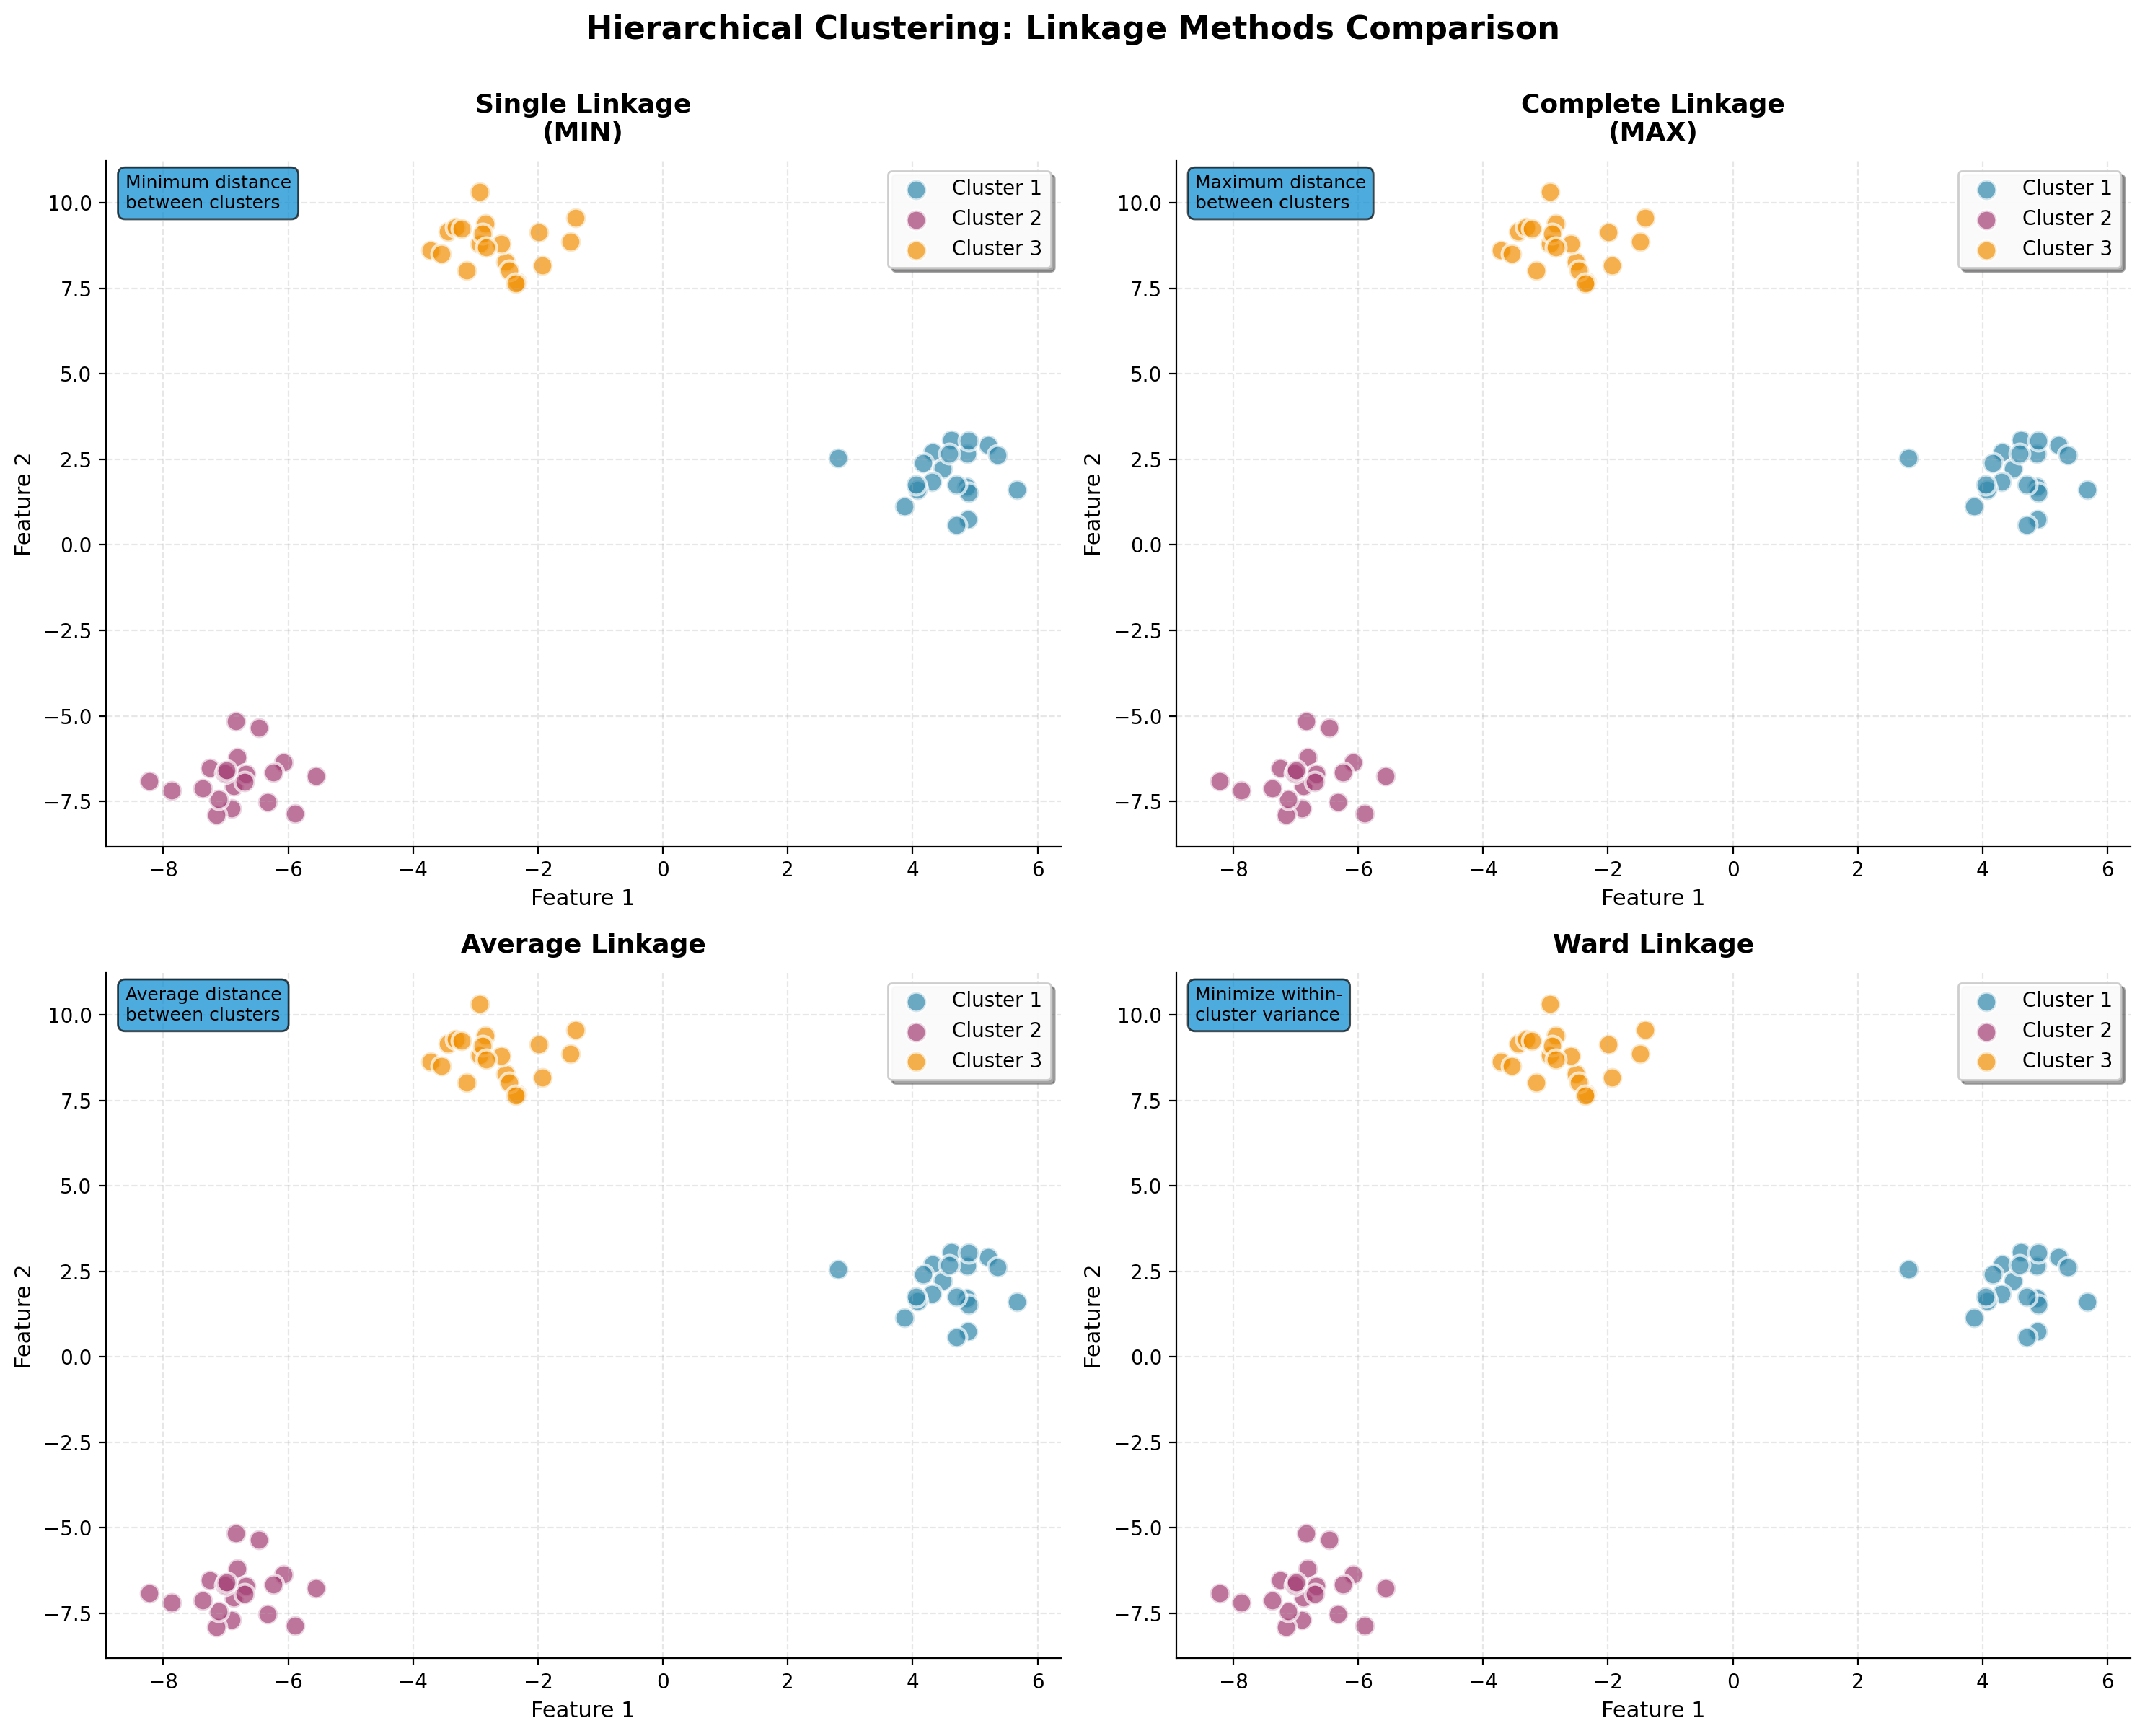
\includegraphics[width=0.85\textwidth]{../figures/linkage_methods_comparison.png}

\vspace{0.15cm}

\begin{columns}[T]
\begin{column}{0.24\textwidth}
\begin{block}{Single}
\begin{itemize}
\setlength{\itemsep}{0pt}
\item Elongated
\item Noise sensitive
\end{itemize}
\end{block}
\end{column}

\begin{column}{0.24\textwidth}
\begin{block}{Complete}
\begin{itemize}
\setlength{\itemsep}{0pt}
\item Compact
\item Outlier sensitive
\end{itemize}
\end{block}
\end{column}

\begin{column}{0.24\textwidth}
\begin{block}{Average}
\begin{itemize}
\setlength{\itemsep}{0pt}
\item Compromise
\item Robust
\end{itemize}
\end{block}
\end{column}

\begin{column}{0.24\textwidth}
\begin{block}{Ward's}
\begin{itemize}
\setlength{\itemsep}{0pt}
\item Min variance
\item \textbf{Most popular}
\end{itemize}
\end{block}
\end{column}
\end{columns}
\end{frame}

\begin{frame}{Dendrograms: Interpretation}
\begin{columns}[T]
\begin{column}{0.45\textwidth}
\begin{block}{Reading Dendrograms}
\begin{itemize}
\setlength{\itemsep}{1pt}
\item \textbf{Leaves}: Individual points
\item \textbf{Height}: Merge distance
\item \textbf{Branches}: Relationships
\item \textbf{Cut}: Extract $K$ clusters
\end{itemize}
\end{block}

\vspace{0.05cm}

\begin{exampleblock}{Extracting Clusters}
Cut at height $h$:
\begin{itemize}
\setlength{\itemsep}{1pt}
\item Higher $\rightarrow$ fewer clusters
\item Lower $\rightarrow$ more clusters
\item Choose via validation
\end{itemize}
\end{exampleblock}

\vspace{0.05cm}

\begin{alertblock}{Advantage}
Explore different $K$ without re-running!
\end{alertblock}
\end{column}

\begin{column}{0.52\textwidth}
\centering
\vspace{0pt}
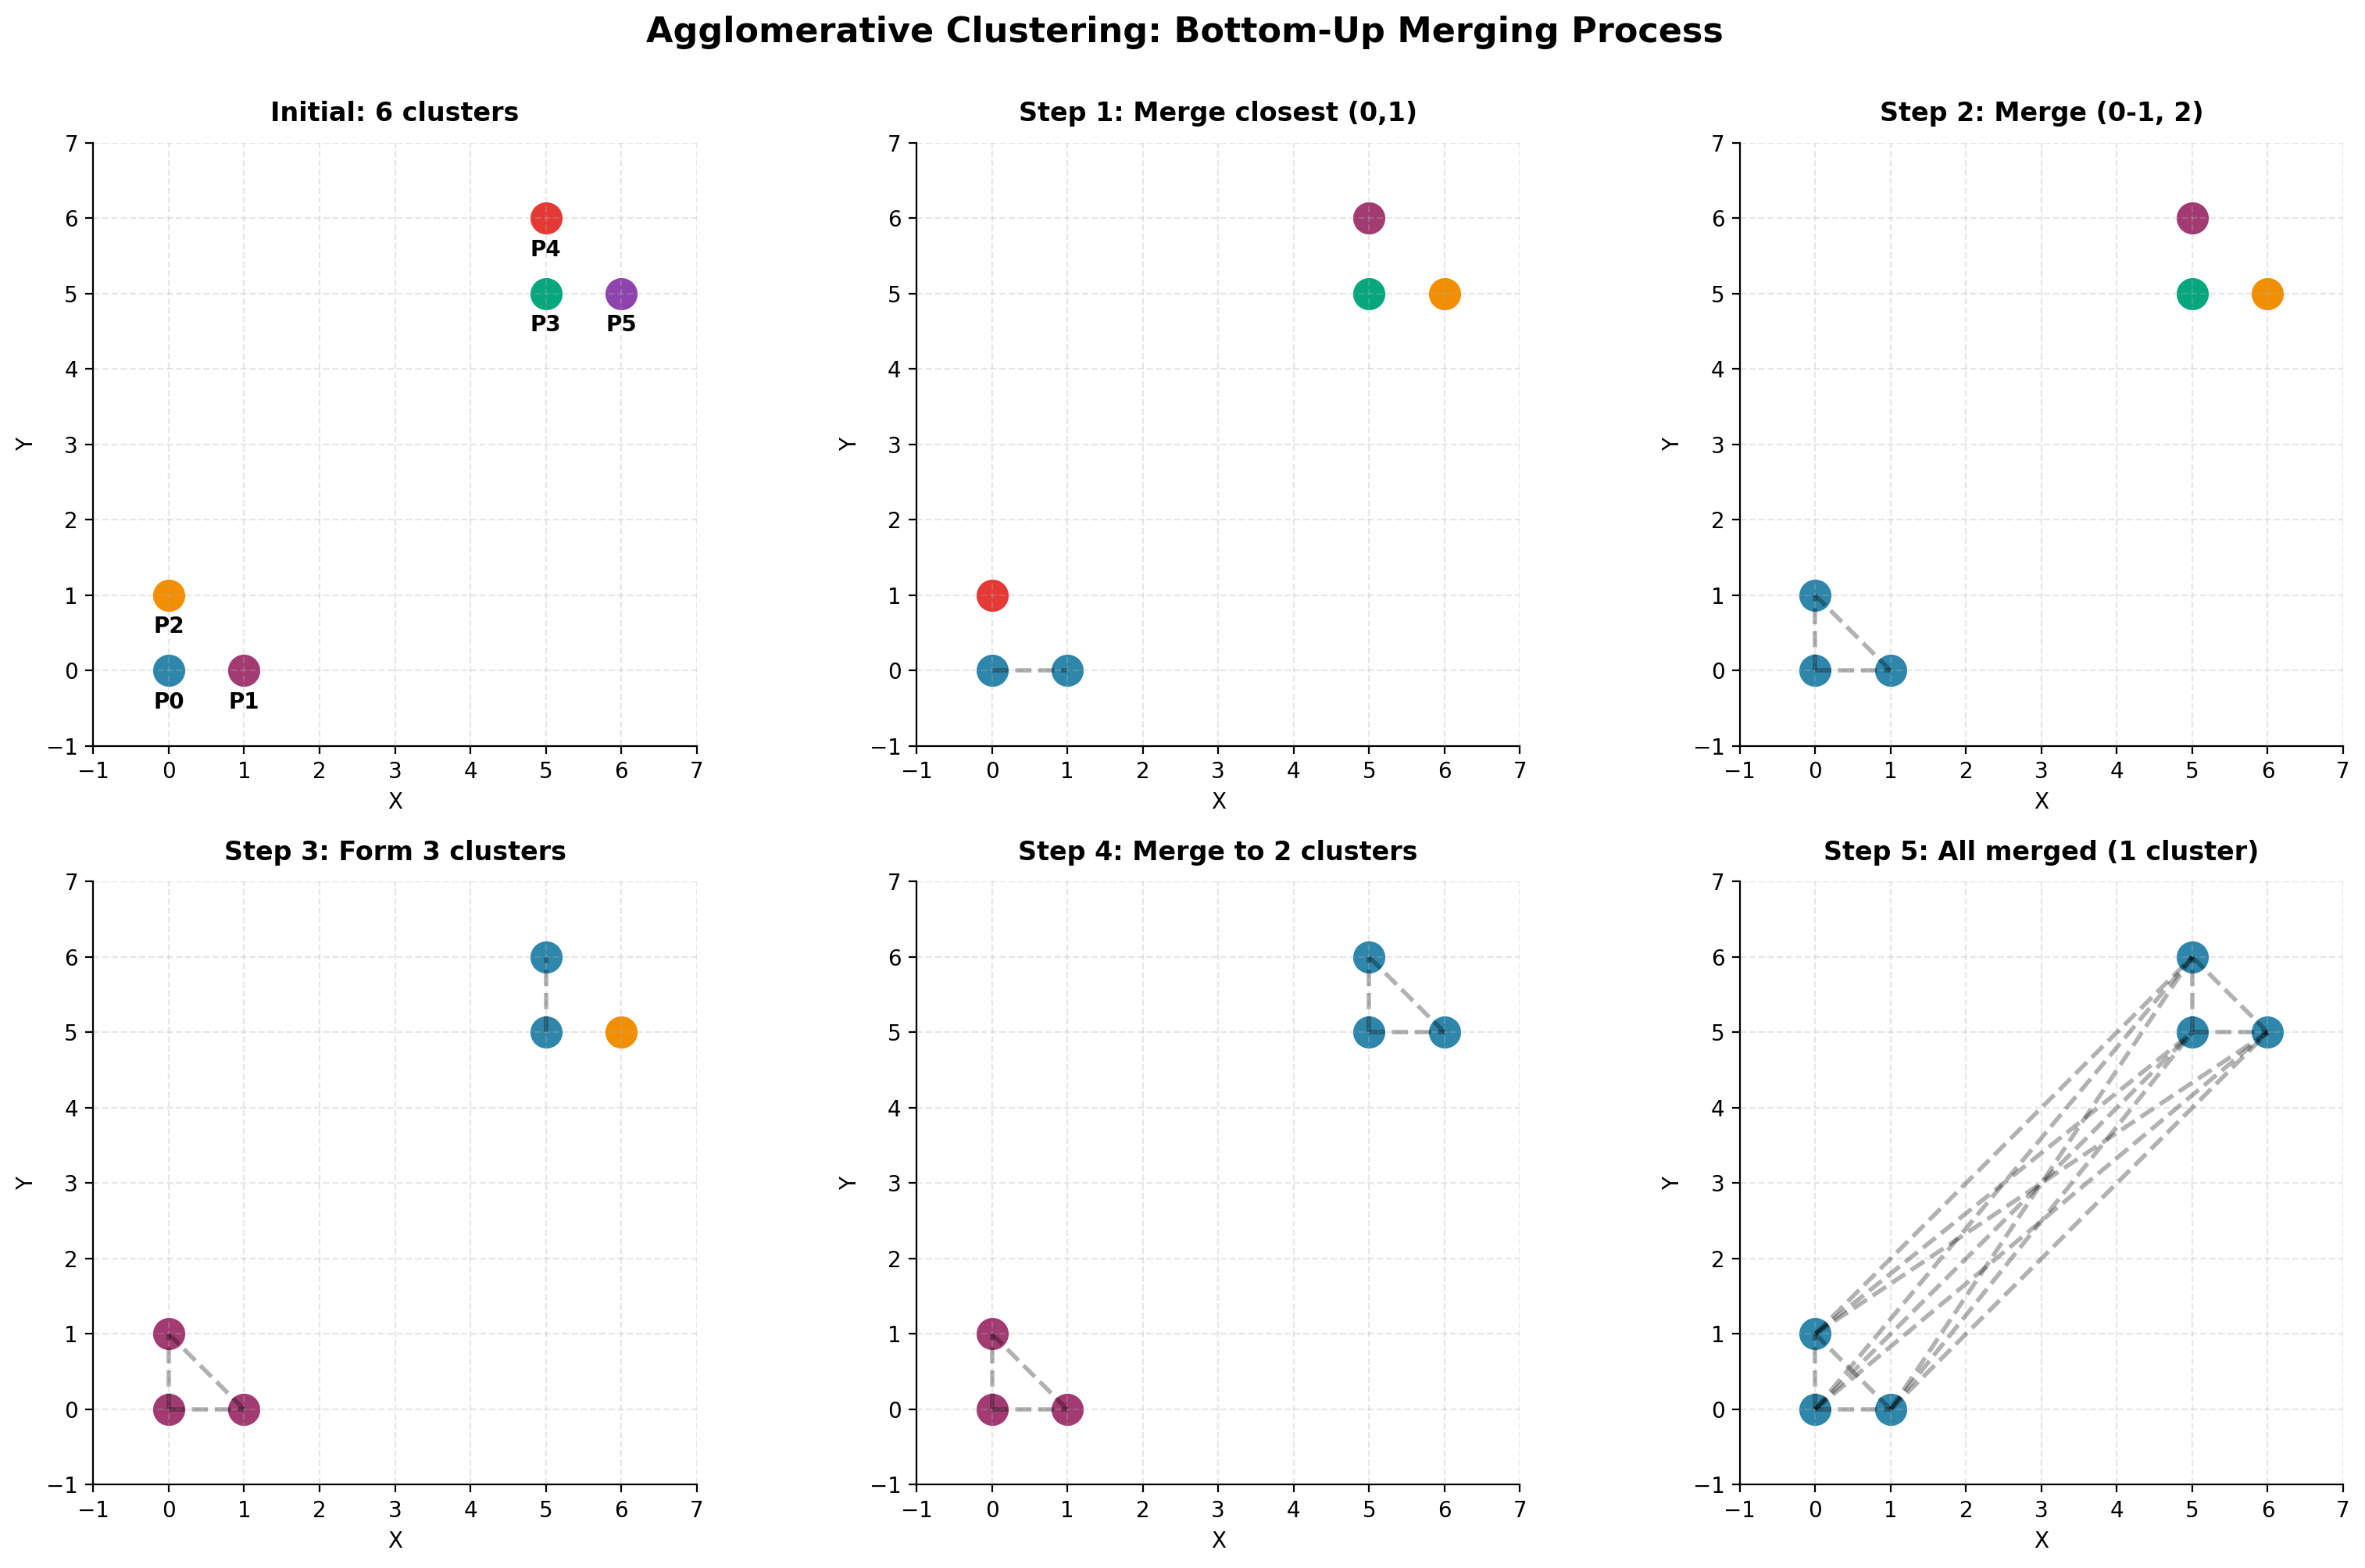
\includegraphics[width=\textwidth]{../figures/agglomerative_steps.png}
\end{column}
\end{columns}
\end{frame}

% ========================================
% Section: Cluster Validation
% ========================================

\section{Cluster Validation \& Evaluation}

\begin{frame}{Types of Cluster Validation}
\textbf{How do we assess clustering quality?}

\vspace{0.2cm}

\begin{columns}[t]
\begin{column}{0.48\textwidth}
\begin{block}{Internal Validation}
\textbf{Use only the data itself}

\vspace{0.1cm}

\textit{Measures:}
\begin{itemize}
\setlength{\itemsep}{2pt}
\item Silhouette coefficient
\item Davies-Bouldin index
\item Calinski-Harabasz score
\item Dunn index
\end{itemize}

\vspace{0.1cm}

\textit{Idea:} Good clusters are compact and well-separated
\end{block}
\end{column}

\begin{column}{0.48\textwidth}
\begin{block}{External Validation}
\textbf{Compare to ground truth labels}

\vspace{0.1cm}

\textit{Measures:}
\begin{itemize}
\setlength{\itemsep}{2pt}
\item Adjusted Rand Index (ARI)
\item Normalized Mutual Information (NMI)
\item V-measure
\item Purity
\end{itemize}

\vspace{0.1cm}

\textit{Idea:} Good clustering agrees with true labels
\end{block}
\end{column}
\end{columns}

\vspace{0.2cm}

\begin{alertblock}{When to Use Each}
\textbf{Internal:} Unsupervised setting (no labels) \quad
\textbf{External:} When ground truth available (benchmarking)
\end{alertblock}
\end{frame}

\begin{frame}{Internal Metrics: Formulas}
\begin{block}{1. Silhouette Coefficient}
$$s = \frac{1}{n} \sum_{i=1}^{n} \frac{b_i - a_i}{\max(a_i, b_i)}$$
Range: $[-1, 1]$, higher is better
\end{block}

\begin{block}{2. Davies-Bouldin Index}
$$DB = \frac{1}{K} \sum_{k=1}^{K} \max_{k' \neq k} \frac{\sigma_k + \sigma_{k'}}{d(\boldsymbol{\mu}_k, \boldsymbol{\mu}_{k'})}$$
Range: $[0, \infty)$, \textbf{lower} is better
\end{block}

\begin{block}{3. Calinski-Harabasz Score (Variance Ratio)}
$$CH = \frac{\text{Between-cluster variance}}{\text{Within-cluster variance}} \times \frac{n - K}{K - 1}$$
Range: $[0, \infty)$, higher is better
\end{block}

\begin{alertblock}{Usage}
Use multiple metrics! Different metrics may favor different clusterings.
\end{alertblock}
\end{frame}

\begin{frame}{Internal Validation: Visualization}

\begin{columns}[T]
\begin{column}{0.48\textwidth}
\centering
\textbf{Metric Values vs K}

\vspace{0.1cm}
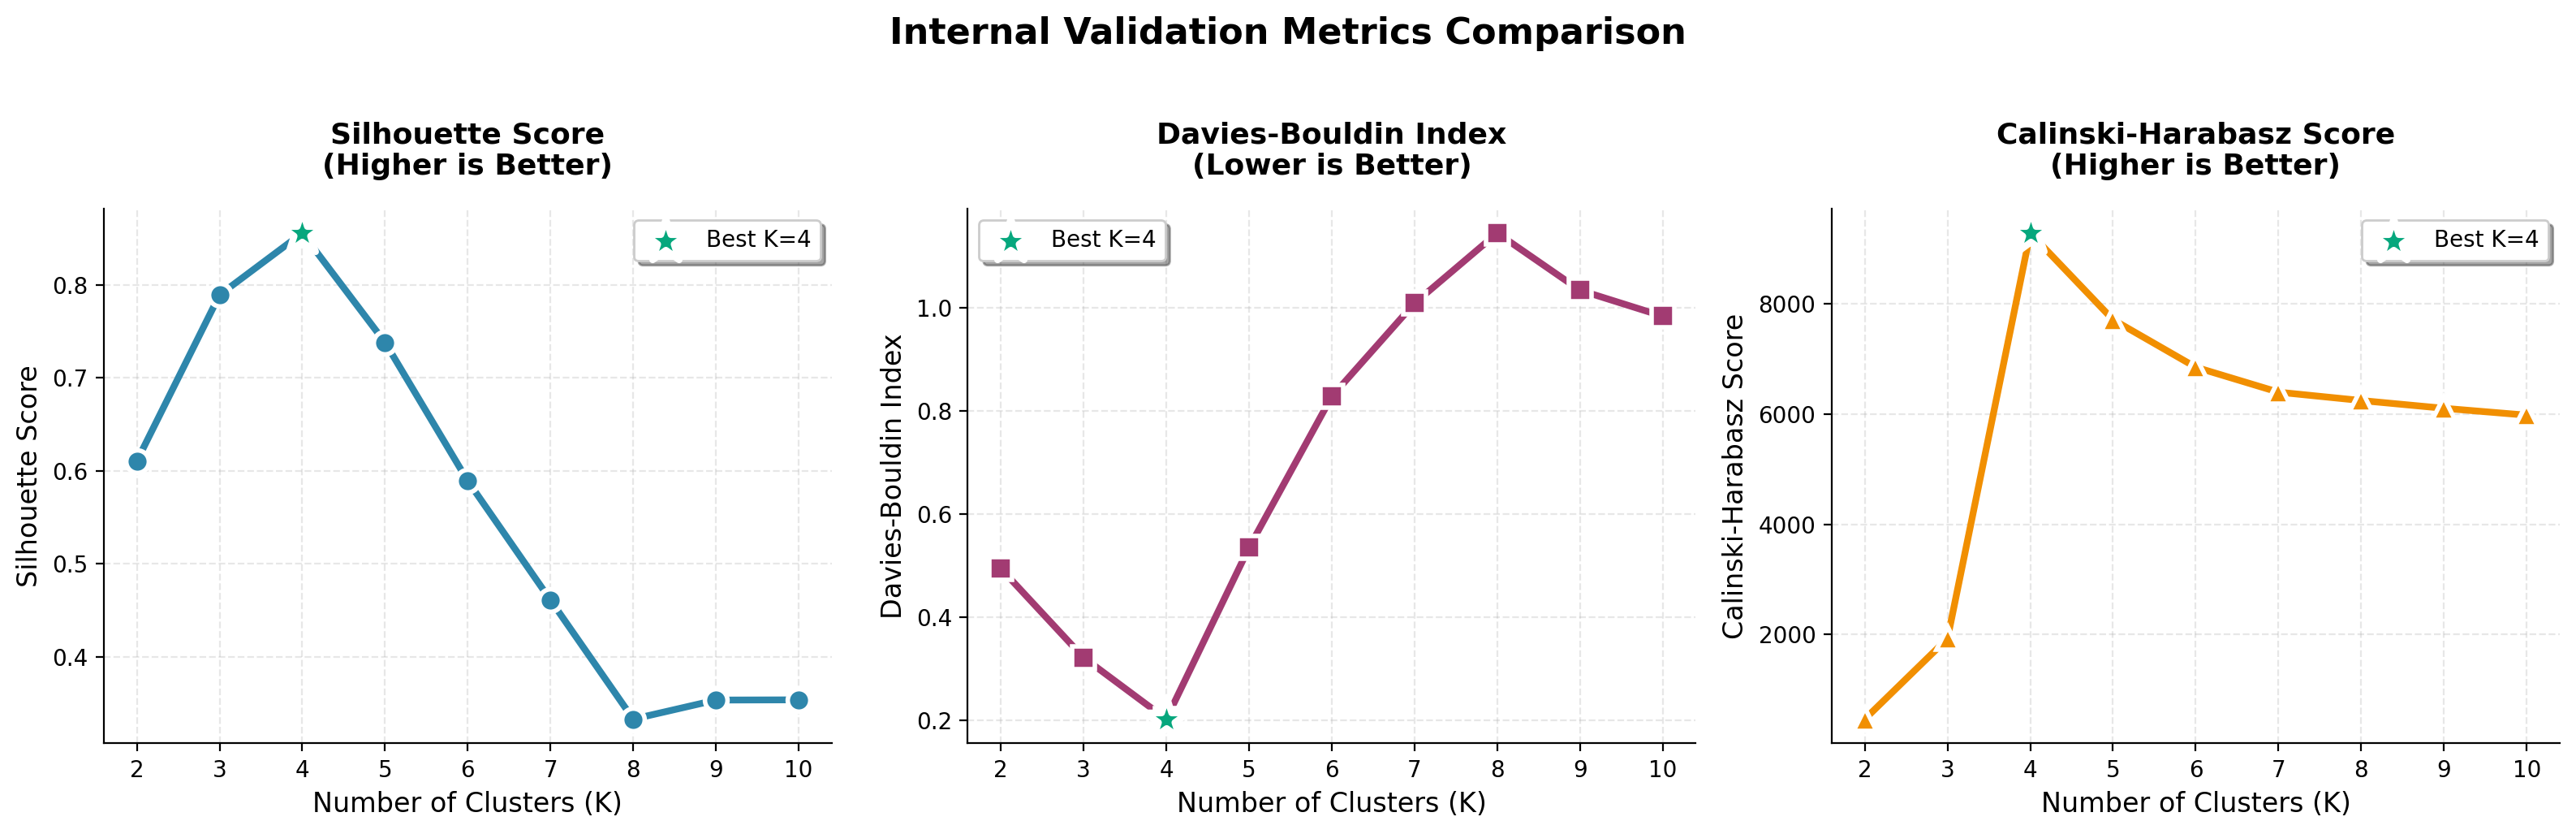
\includegraphics[width=\textwidth]{../figures/internal_validation_metrics.png}
\end{column}

\begin{column}{0.48\textwidth}
\centering
\textbf{Optimal K Comparison}

\vspace{0.1cm}
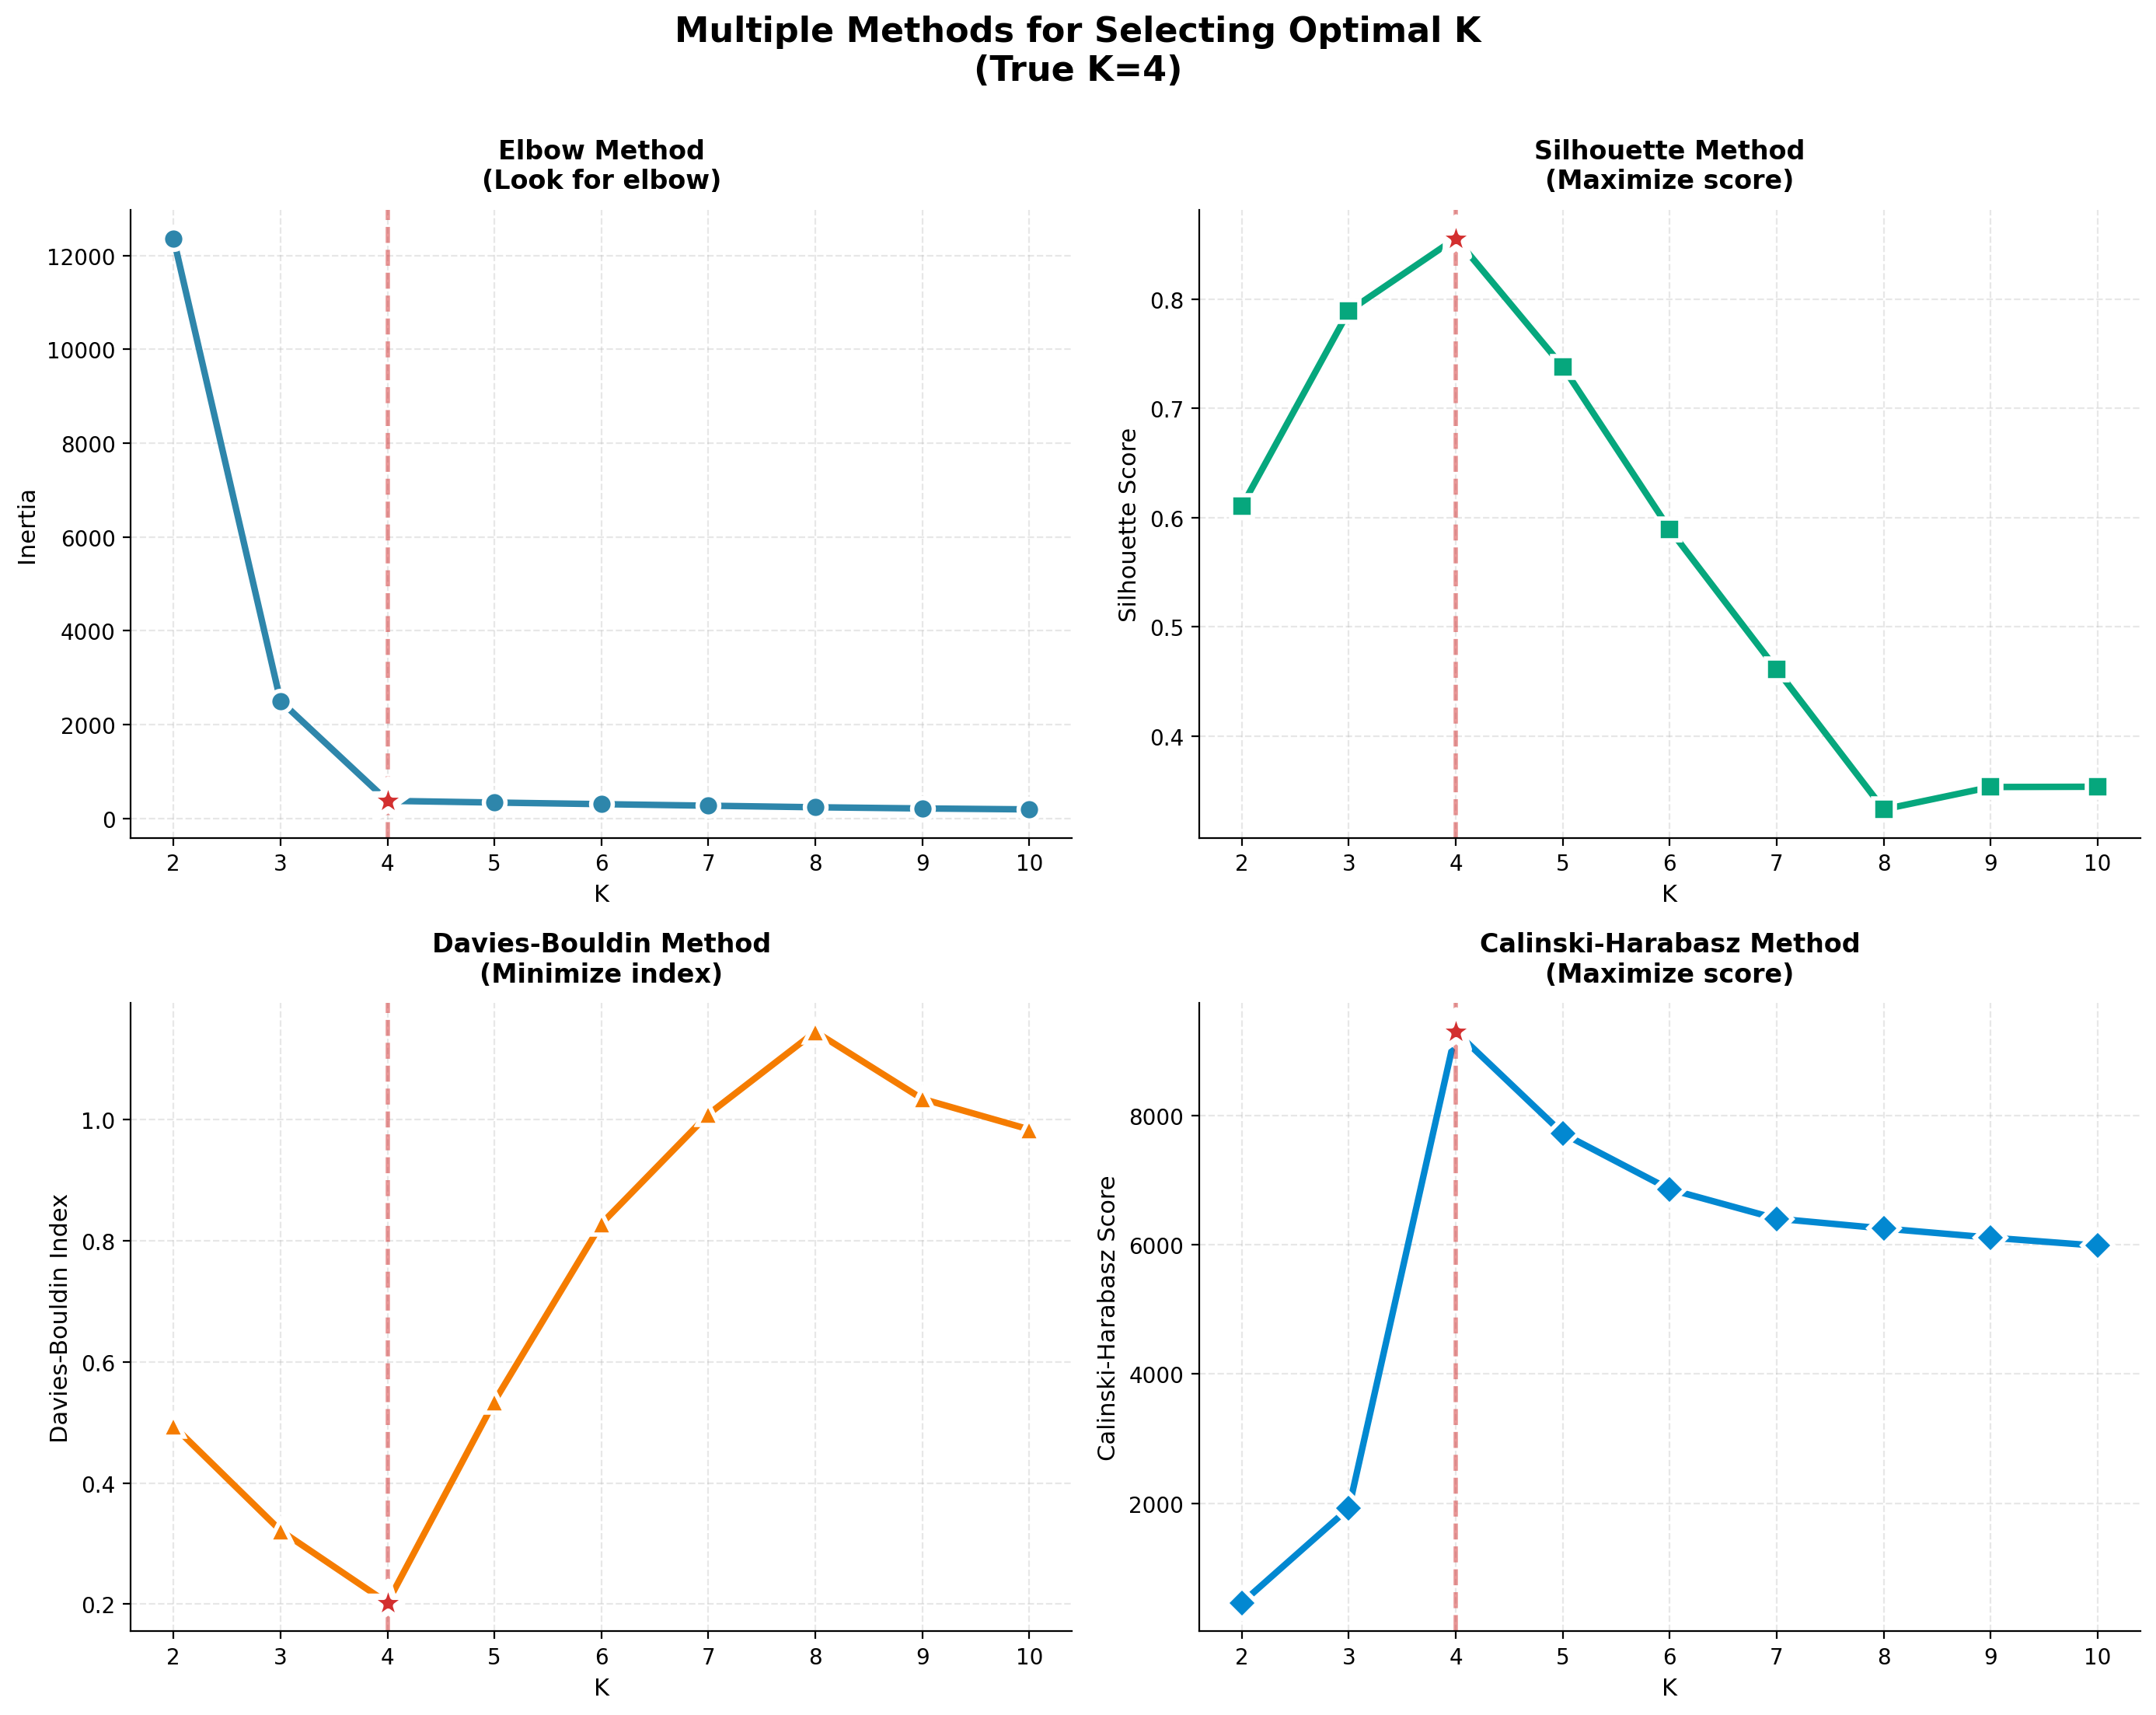
\includegraphics[width=\textwidth]{../figures/optimal_k_comparison.png}
\end{column}
\end{columns}

\vspace{0.15cm}

\begin{alertblock}{Observation}
Different metrics may suggest different optimal $K$. Use domain knowledge!
\end{alertblock}
\end{frame}

\begin{frame}{External Metrics: Formulas}
\textbf{Given true labels $Y$ and predicted labels $C$:}

\vspace{0.2cm}

\begin{block}{1. Adjusted Rand Index (ARI)}
$$ARI = \frac{\text{RI} - E[\text{RI}]}{\max(\text{RI}) - E[\text{RI}]}$$

\begin{itemize}
\item Range: $[-1, 1]$, higher is better
\item $ARI = 1$: Perfect agreement
\item $ARI \approx 0$: Random labeling
\item Adjusted for chance
\end{itemize}
\end{block}

\begin{block}{2. Normalized Mutual Information (NMI)}
$$NMI(Y, C) = \frac{2 \cdot I(Y; C)}{H(Y) + H(C)}$$

\begin{itemize}
\item Range: $[0, 1]$, higher is better
\item $NMI = 1$: Perfect agreement
\item Based on information theory
\item Normalized for different $K$
\end{itemize}
\end{block}
\end{frame}

\begin{frame}{External Validation: Example}

\begin{columns}[T]
\begin{column}{0.48\textwidth}
\centering
\textbf{Validation Metrics}

\vspace{0.1cm}
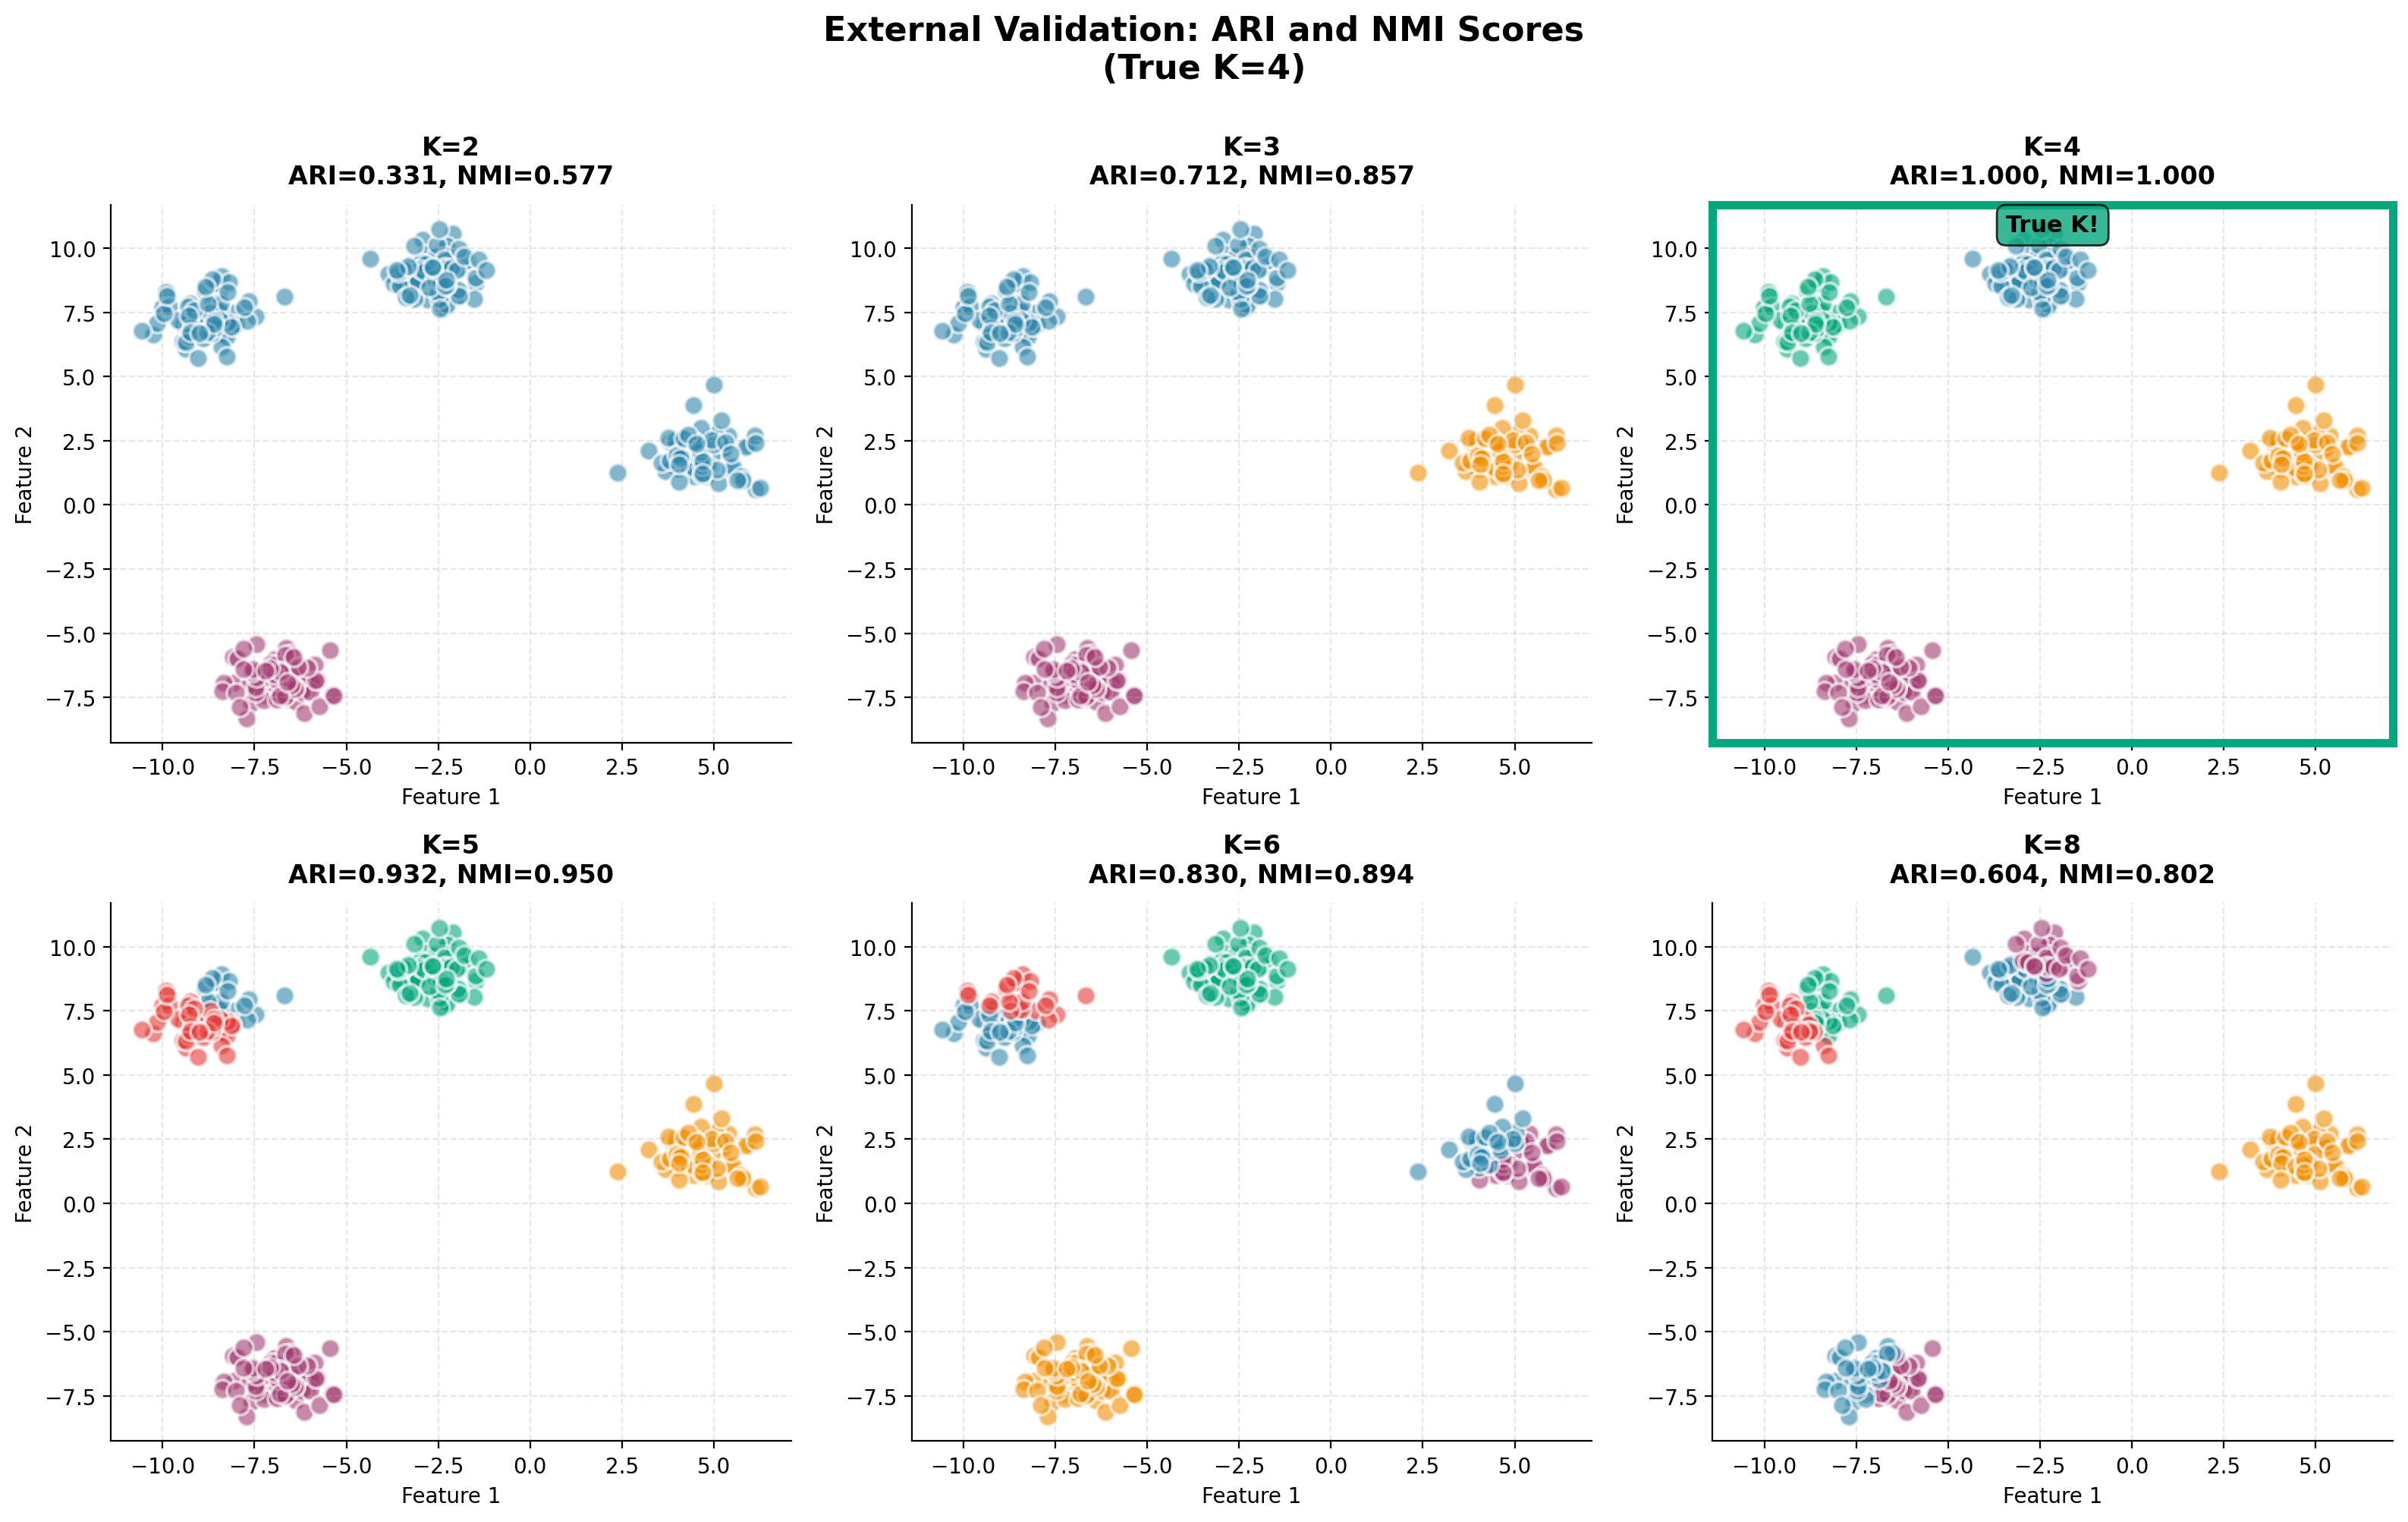
\includegraphics[width=\textwidth]{../figures/external_validation_metrics.png}
\end{column}

\begin{column}{0.48\textwidth}
\centering
\textbf{Confusion Matrix}

\vspace{0.1cm}
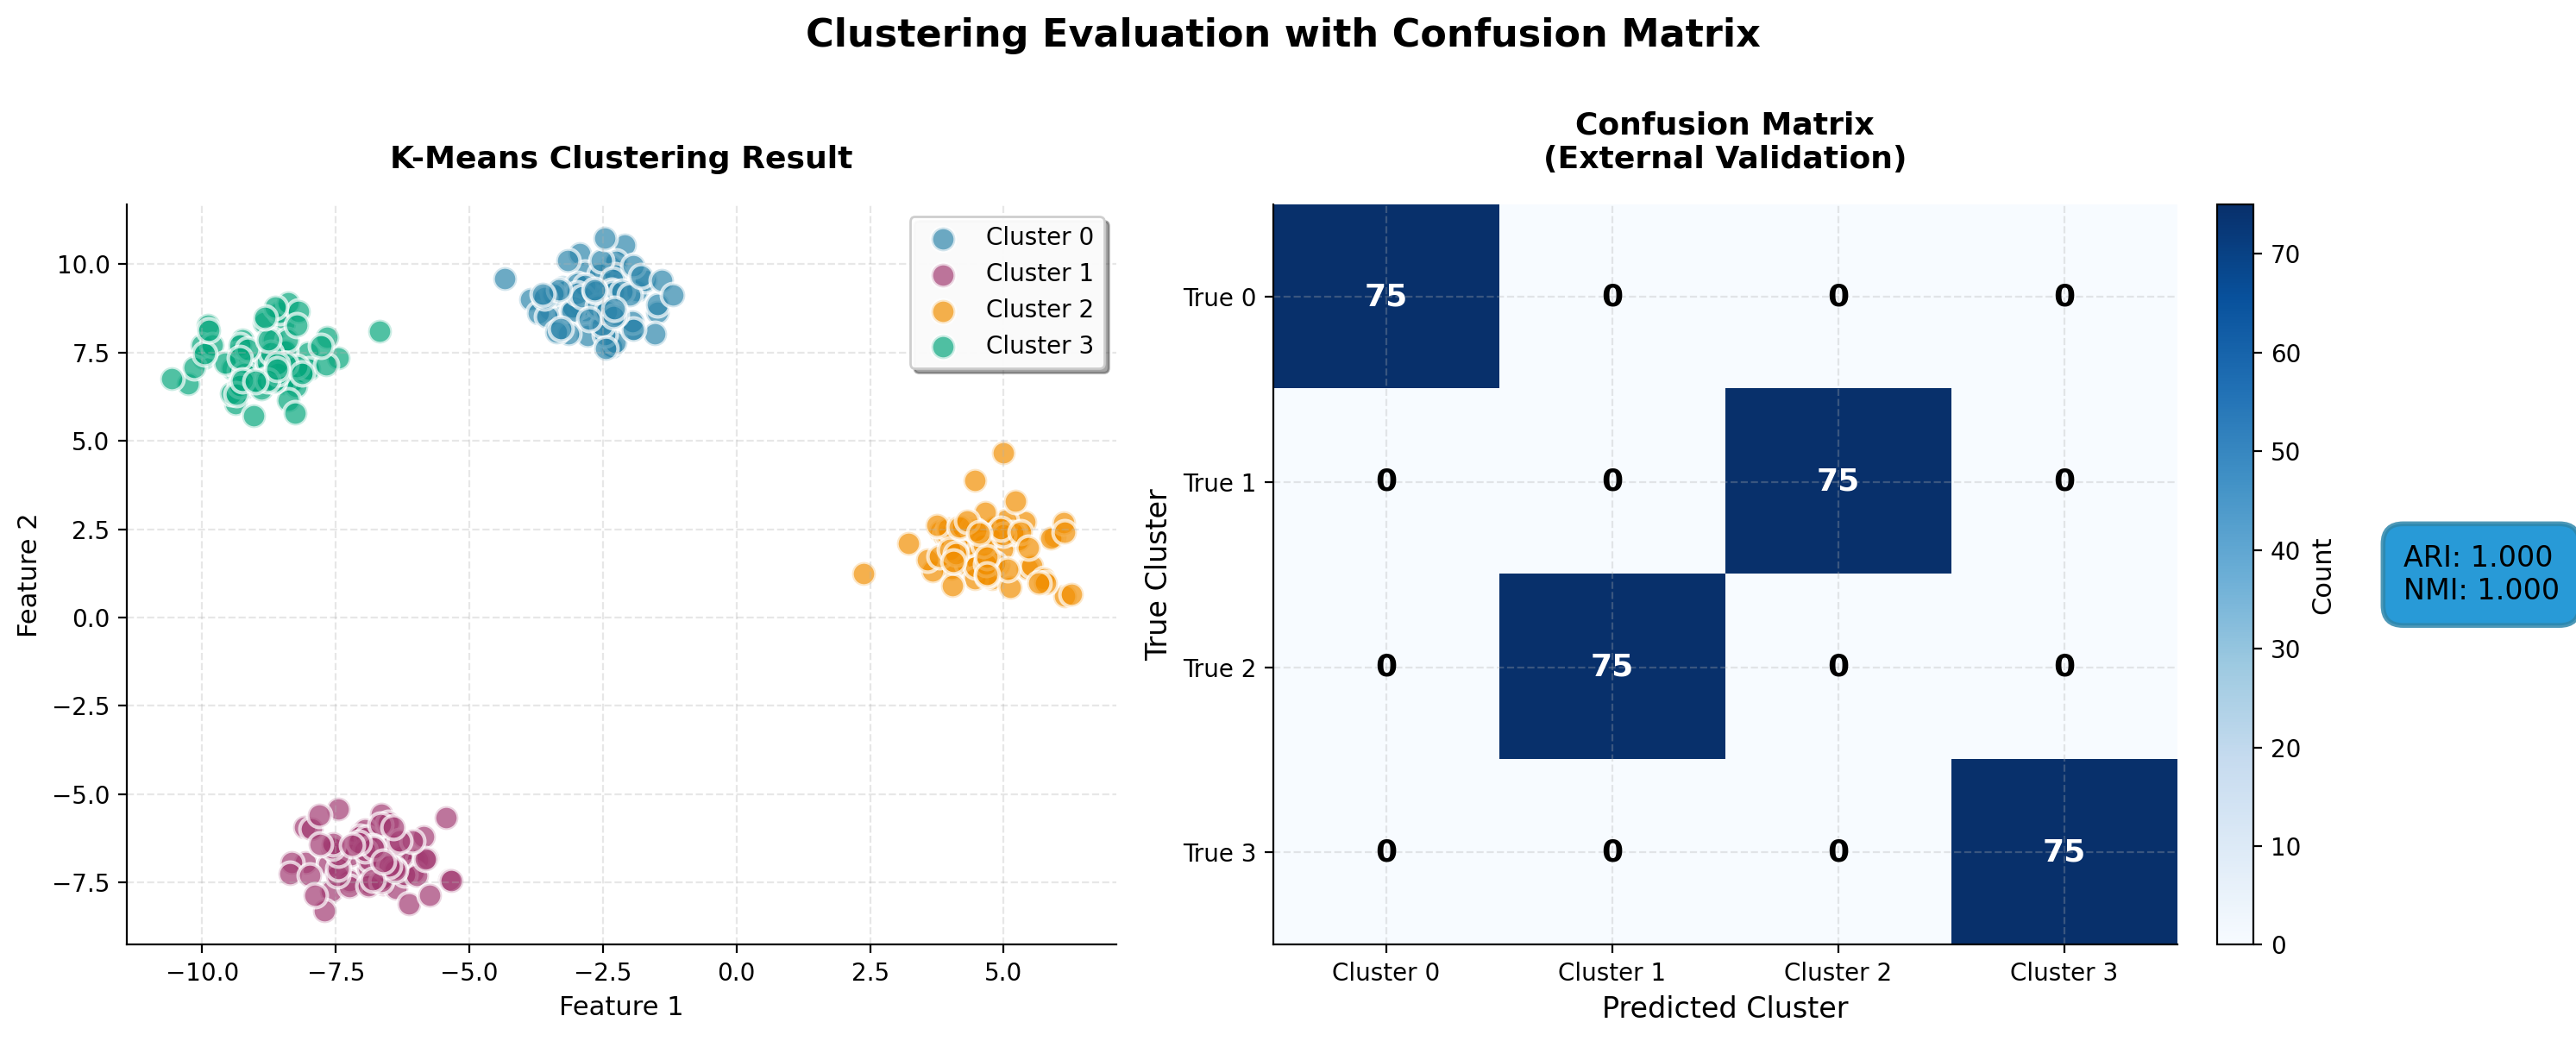
\includegraphics[width=\textwidth]{../figures/clustering_confusion_matrix.png}
\end{column}
\end{columns}

\vspace{0.15cm}

\begin{alertblock}{Note}
External validation only for benchmarking. In real unsupervised tasks, no ground truth!
\end{alertblock}
\end{frame}

% ========================================
% Section: Applications
% ========================================

\section{Real-World Applications}

\begin{frame}{Application: Customer Segmentation}
\centering
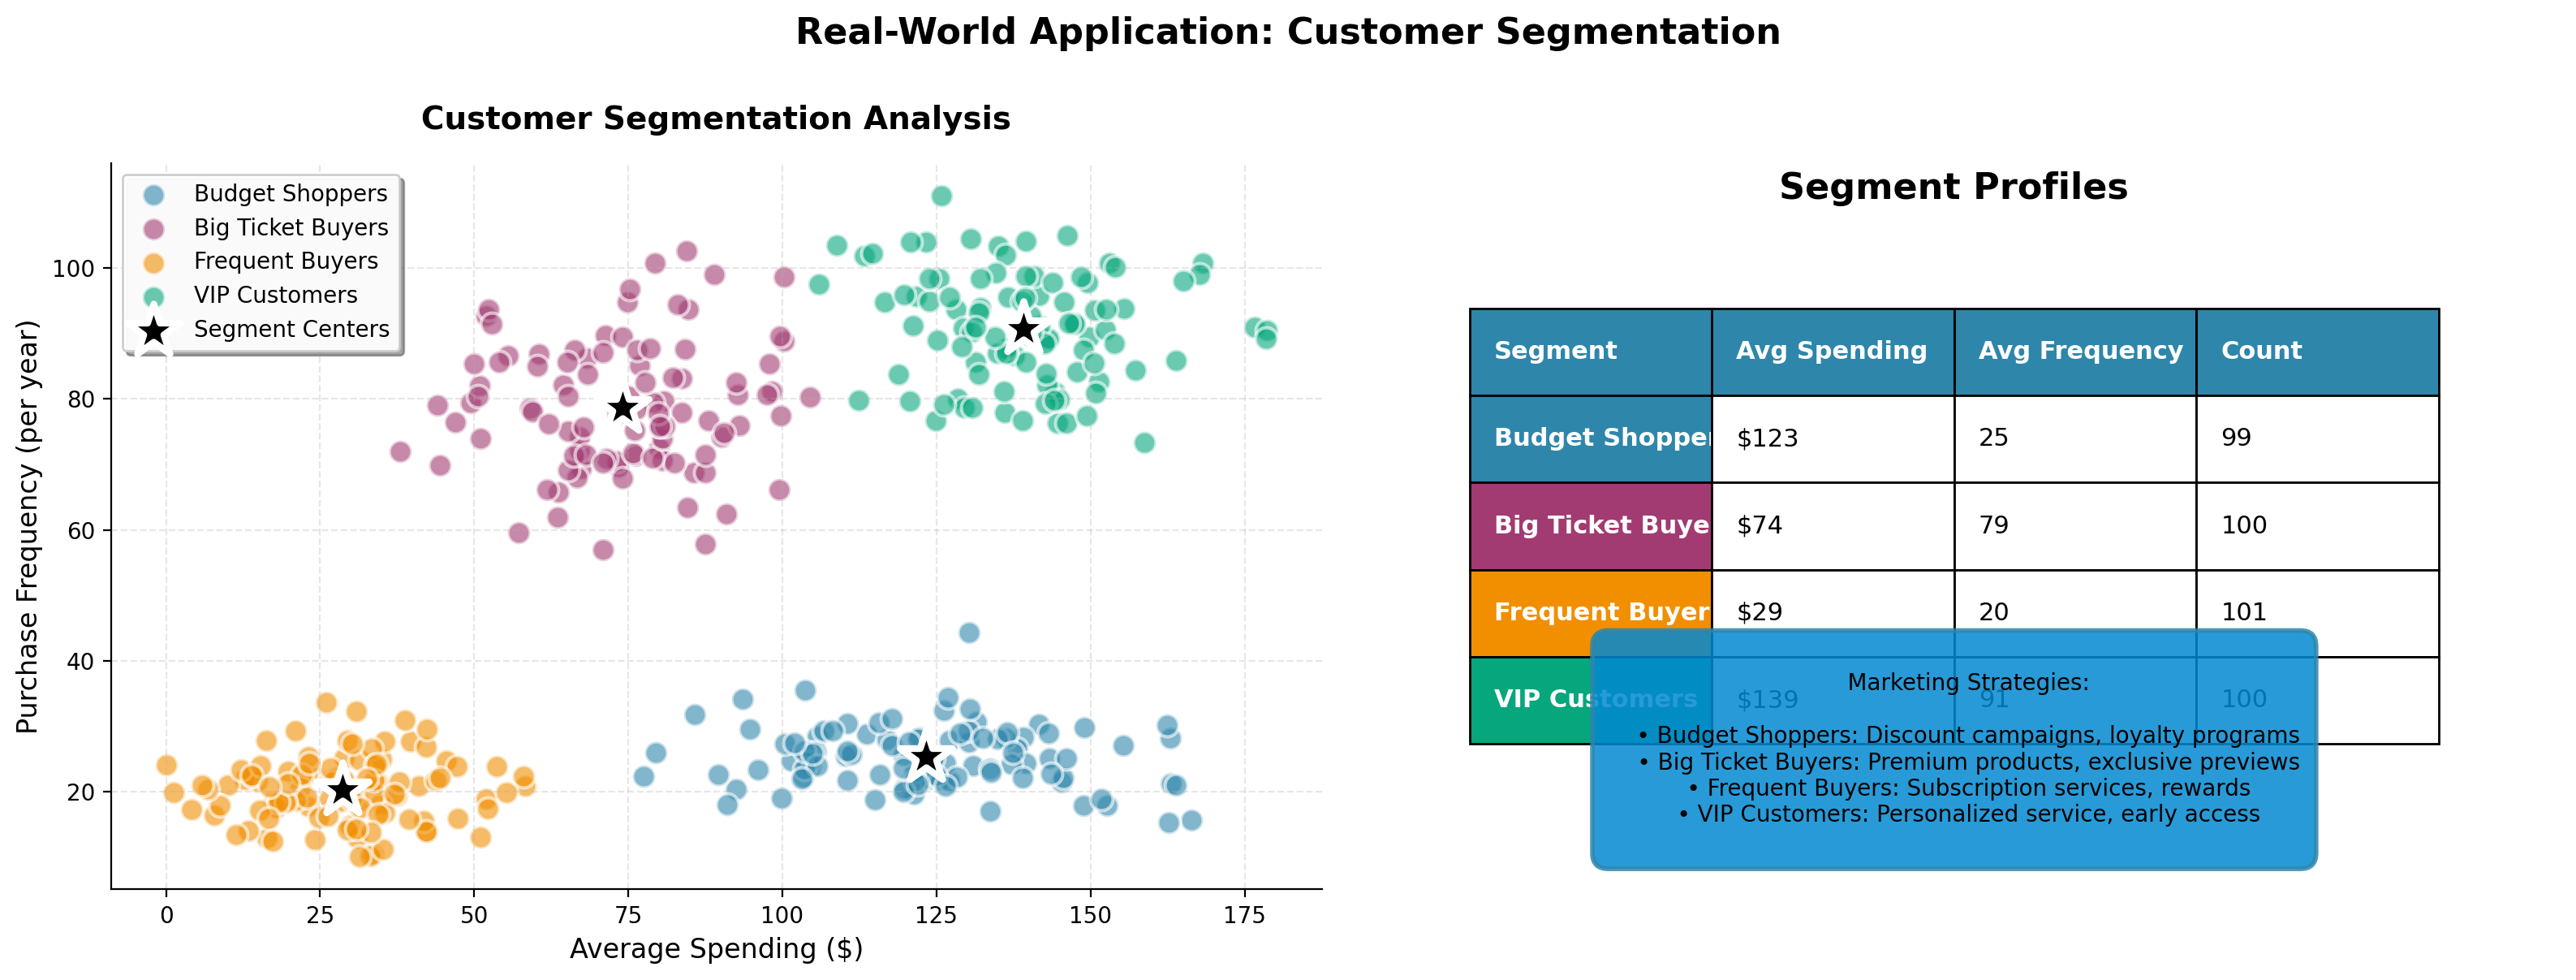
\includegraphics[width=0.85\textwidth]{../figures/customer_segmentation.png}

\vspace{0.12cm}

\begin{exampleblock}{Business Impact}
\begin{itemize}
\setlength{\itemsep}{0pt}
\item \textbf{Targeted marketing}: Strategies per segment
\item \textbf{Product development}: Tailor to groups
\item \textbf{Resource allocation}: Focus on high-value
\item \textbf{Customer retention}: Identify at-risk
\end{itemize}
\end{exampleblock}
\end{frame}

\begin{frame}{Application: Image Color Quantization}
\centering
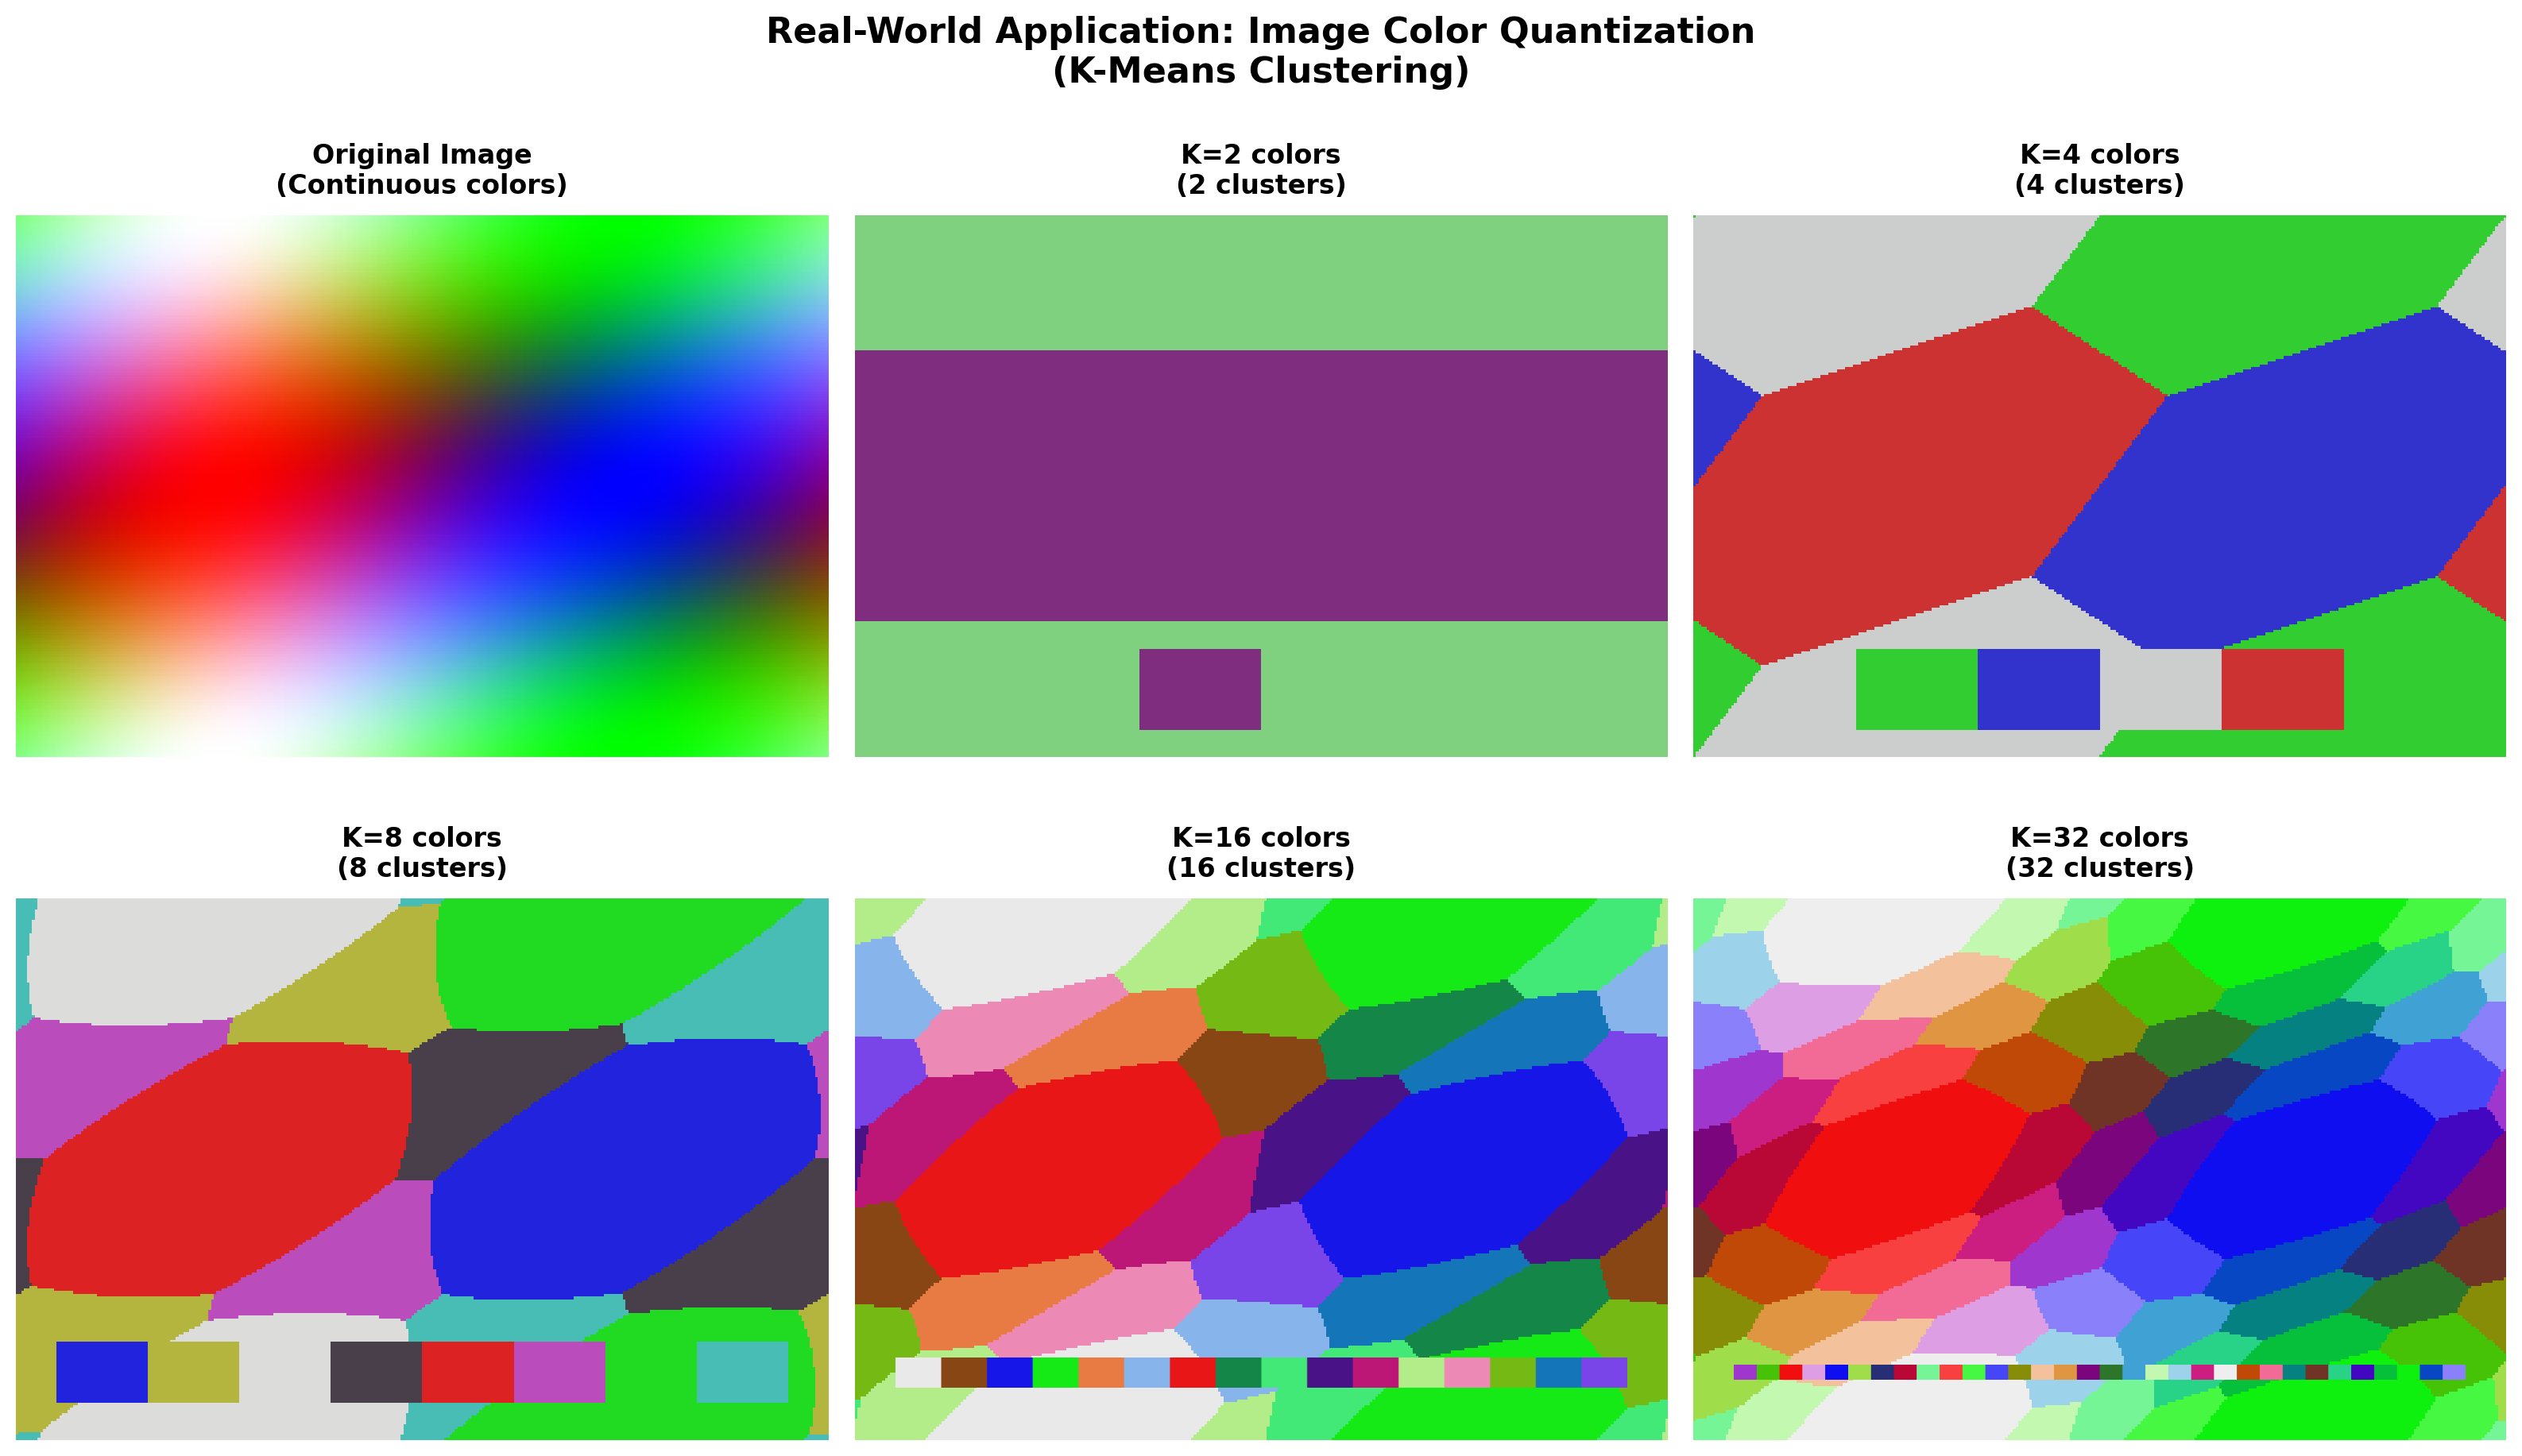
\includegraphics[width=0.82\textwidth]{../figures/image_color_quantization.png}

\vspace{0.12cm}

\begin{exampleblock}{Use Cases}
\begin{itemize}
\setlength{\itemsep}{0pt}
\item \textbf{Image compression}: Reduce file size
\item \textbf{Color palette}: Identify dominant colors
\item \textbf{Segmentation}: Group similar pixels
\item \textbf{Artistic effects}: Posterization
\end{itemize}
\end{exampleblock}
\end{frame}

\begin{frame}{Application: Biological Data (Iris Dataset)}
\centering
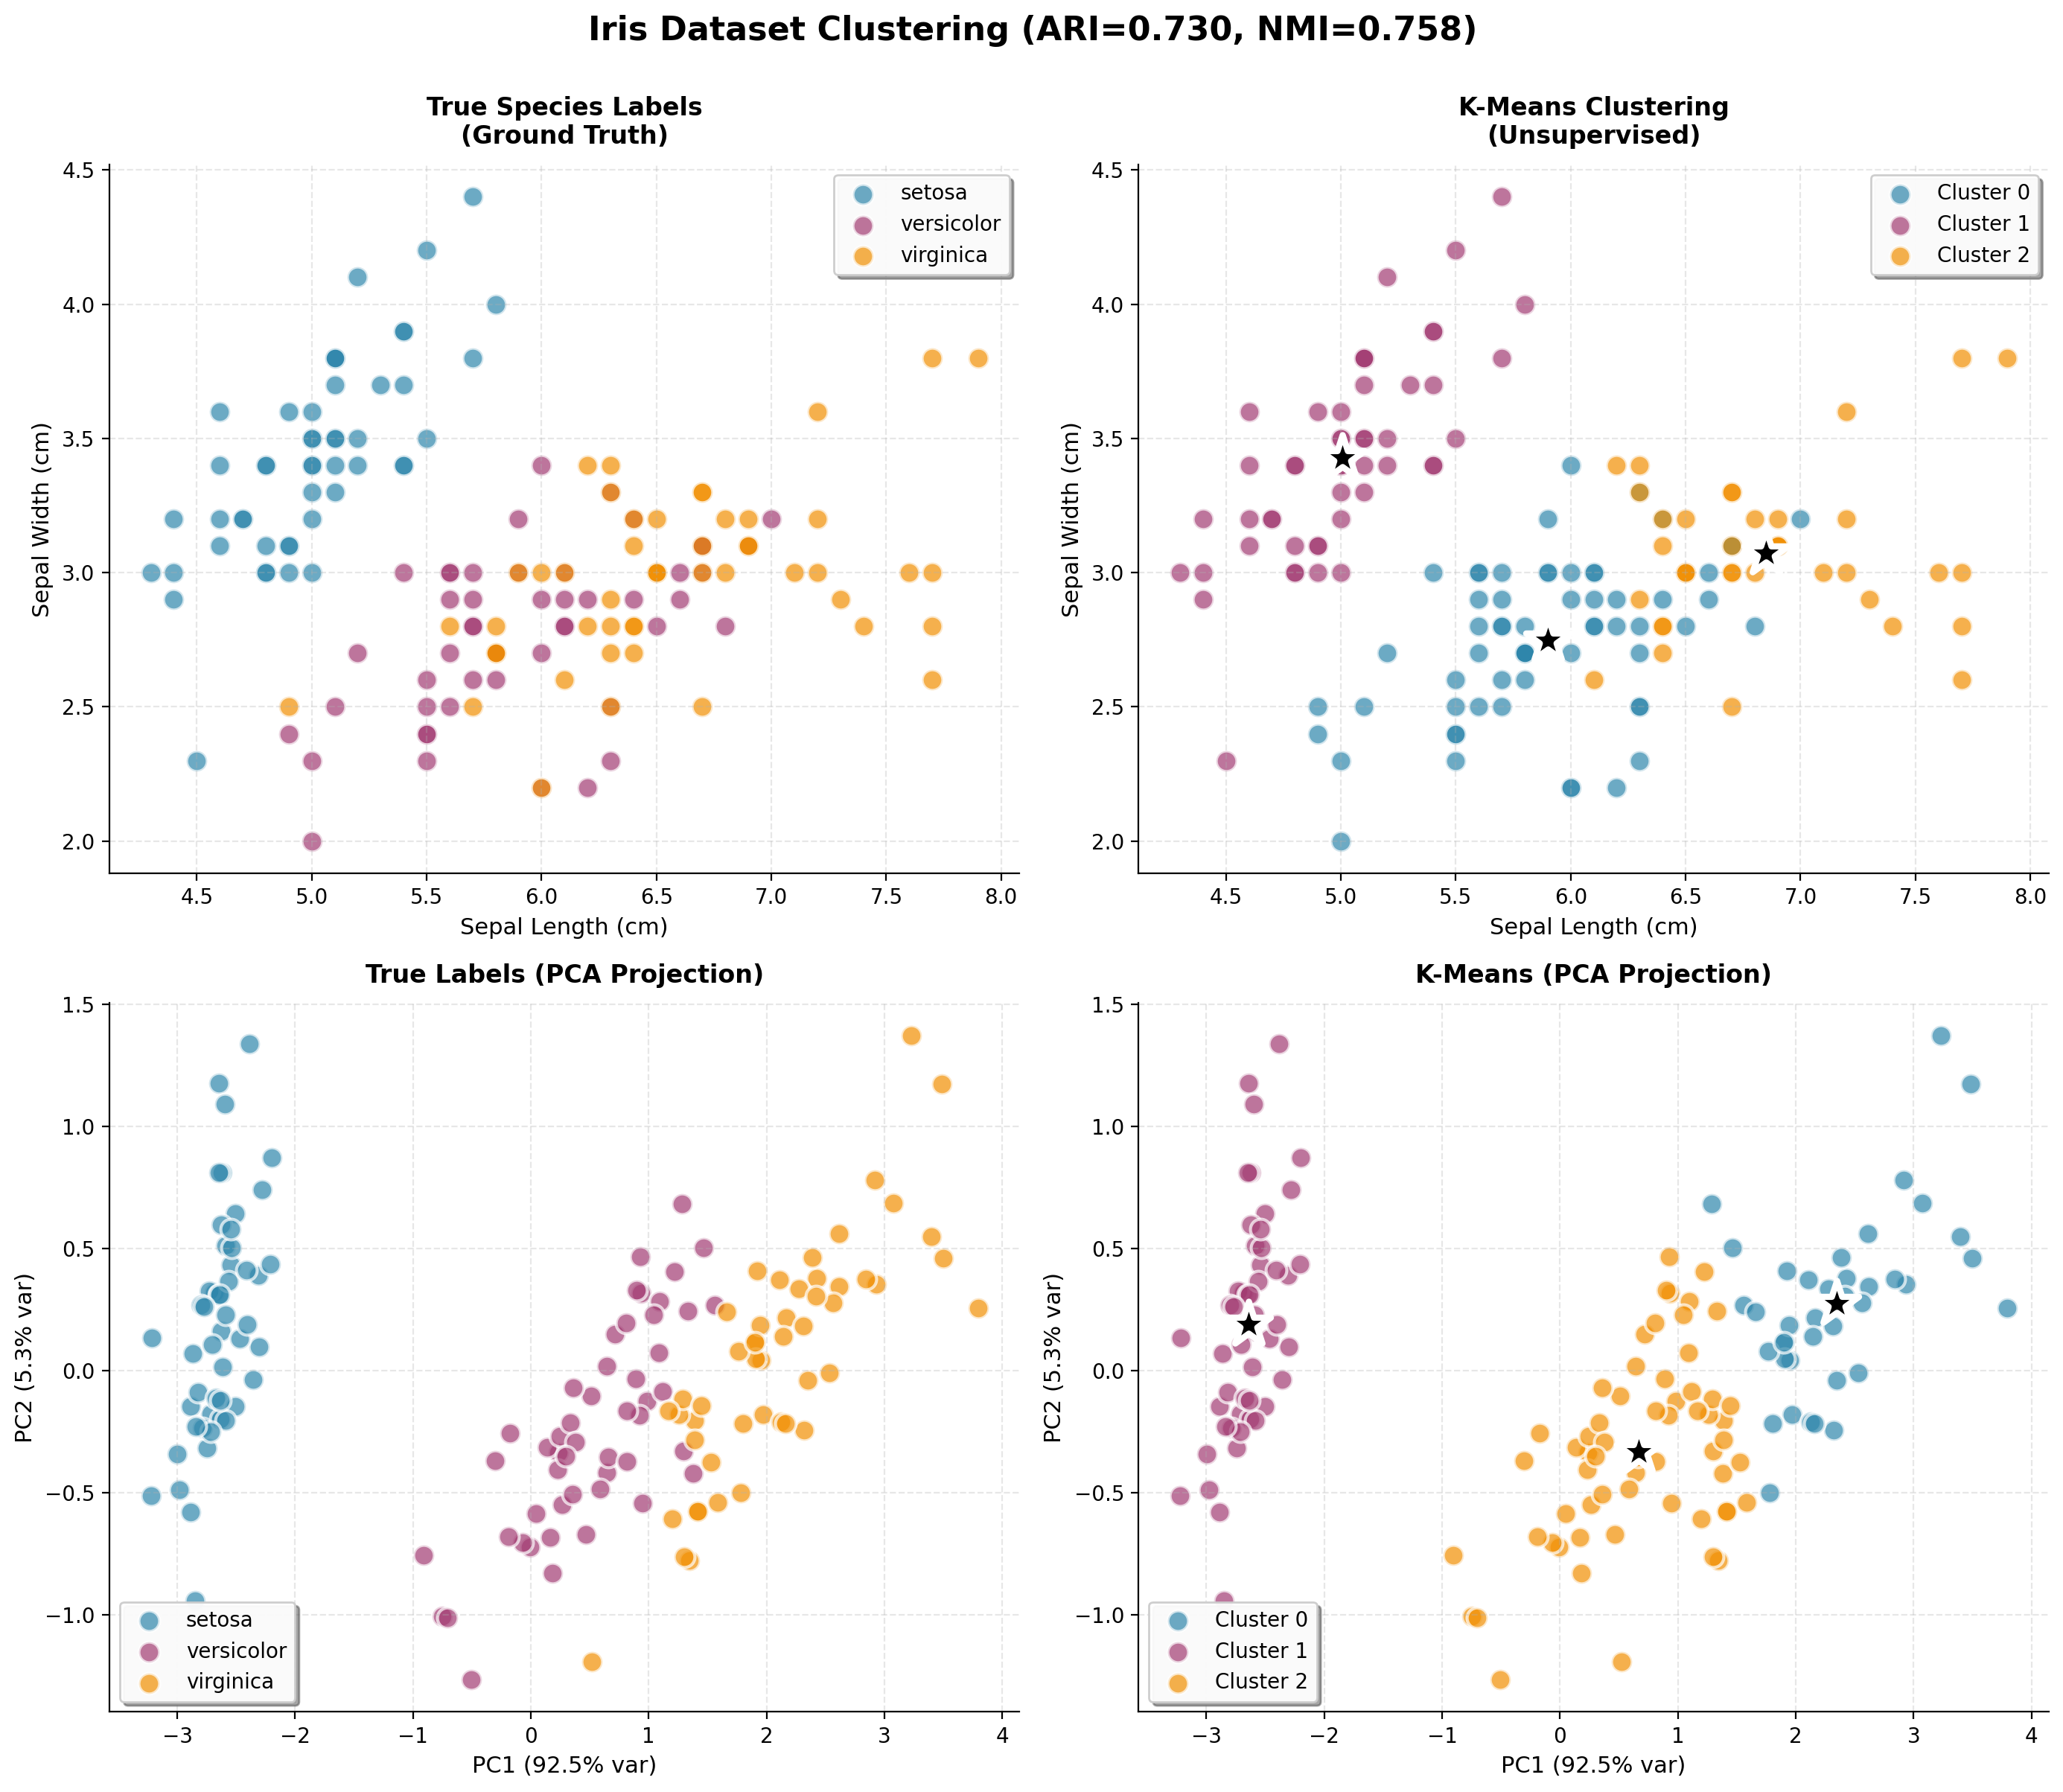
\includegraphics[width=0.88\textwidth]{../figures/iris_species_clustering.png}

\vspace{0.04cm}

\begin{exampleblock}{Bioinformatics Applications}
\begin{itemize}
\setlength{\itemsep}{0pt}
\item \textbf{Species classification}: Taxonomic groups
\item \textbf{Gene expression}: Co-expressed genes
\item \textbf{Protein structure}: Protein families
\item \textbf{Disease subtyping}: Patient subtypes
\end{itemize}
\end{exampleblock}
\end{frame}

\begin{frame}{Application: Document Clustering}
\centering
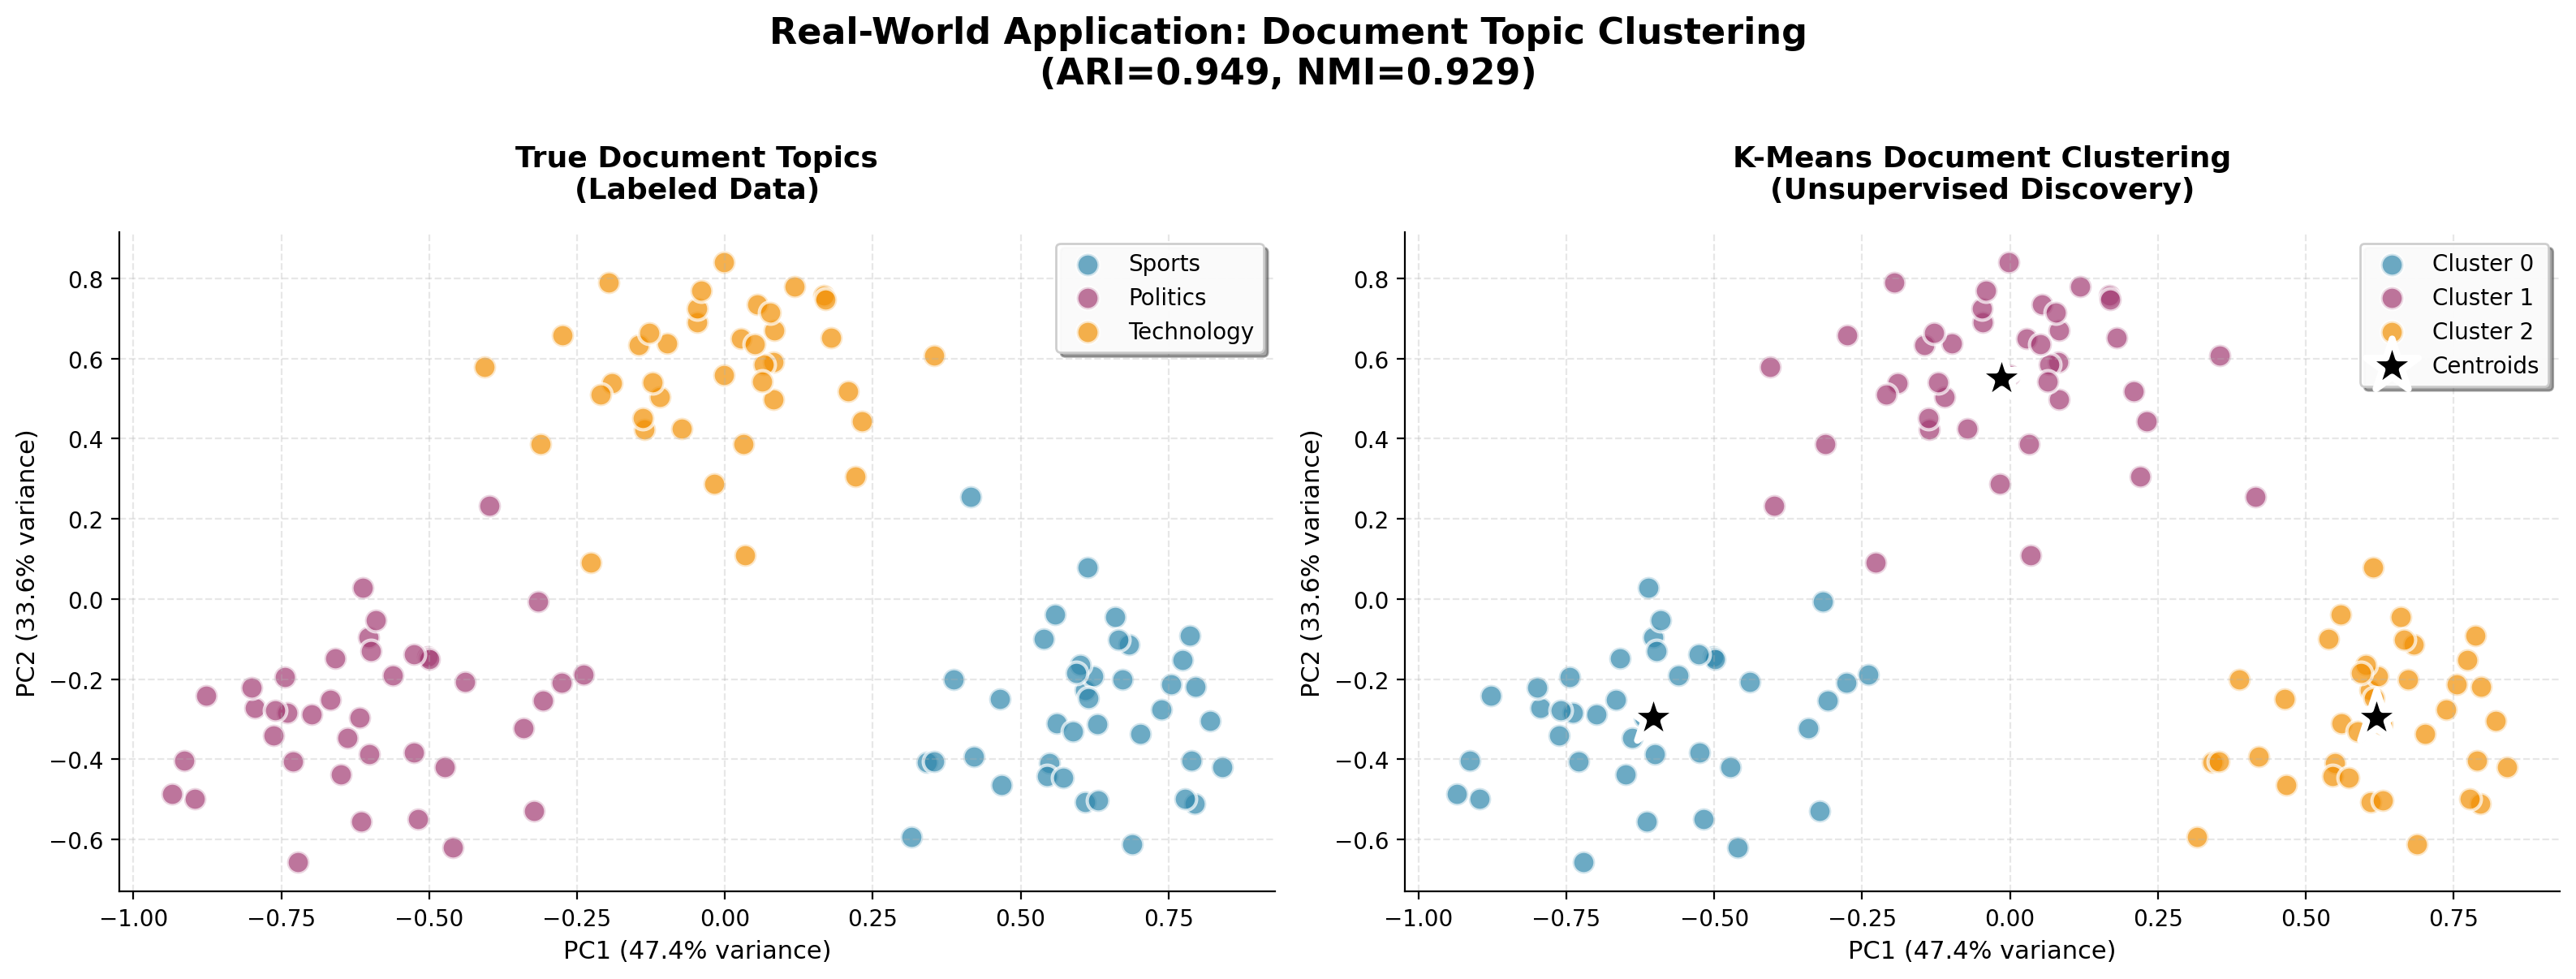
\includegraphics[width=0.92\textwidth]{../figures/document_clustering.png}

\vspace{0.08cm}

\begin{exampleblock}{Text Mining Applications}
\begin{itemize}
\item \textbf{Topic discovery}: Find themes in document collections
\item \textbf{News organization}: Group similar articles
\item \textbf{Search results}: Organize by topic clusters
\item \textbf{Recommendation}: Find similar documents
\end{itemize}
\end{exampleblock}
\end{frame}

% ========================================
% Section: Best Practices
% ========================================

\section{Best Practices \& Guidelines}

\begin{frame}{Choosing a Clustering Algorithm}
\begin{block}{Decision Guide}
\textbf{Use K-Means when:}
\begin{itemize}
\setlength{\itemsep}{2pt}
\item You know $K$ (or can estimate it)
\item Data has roughly spherical clusters
\item Large dataset (scalability important)
\item Want fast, simple method
\end{itemize}

\vspace{0.15cm}

\textbf{Use GMM when:}
\begin{itemize}
\setlength{\itemsep}{2pt}
\item Need probabilistic assignments
\item Clusters have different shapes/variances
\item Want to measure uncertainty
\item Have computational resources
\end{itemize}

\vspace{0.15cm}

\textbf{Use Hierarchical when:}
\begin{itemize}
\setlength{\itemsep}{2pt}
\item Don't know $K$ in advance
\item Want to explore multiple granularities
\item Need interpretable hierarchy
\item Small to medium dataset ($n < 10,000$)
\end{itemize}
\end{block}
\end{frame}

\begin{frame}{Common Pitfalls \& Solutions}
\begin{block}{Pitfall 1: Not Scaling Features}
\textbf{Problem:} Features with large ranges dominate distance

\textbf{Solution:} Standardize features: $z = \frac{x - \mu}{\sigma}$
\end{block}

\begin{block}{Pitfall 2: Using Wrong Distance Metric}
\textbf{Problem:} Euclidean not always appropriate

\textbf{Solution:} Match metric to data type (cosine for text, custom for categorical)
\end{block}

\begin{block}{Pitfall 3: Ignoring Outliers}
\textbf{Problem:} Outliers can distort clusters (especially K-Means)

\textbf{Solution:} Detect and remove outliers, or use robust methods (DBSCAN, K-Medoids)
\end{block}

\begin{block}{Pitfall 4: Blindly Trusting One Metric}
\textbf{Problem:} Single validation metric may be misleading

\textbf{Solution:} Use multiple metrics + visual inspection + domain knowledge
\end{block}
\end{frame}

\begin{frame}{Best Practices: Practical Tips}
\begin{exampleblock}{Data Preprocessing}
\begin{itemize}
\setlength{\itemsep}{2pt}
\item \textbf{Scale features}: Use StandardScaler or MinMaxScaler
\item \textbf{Handle missing values}: Impute or remove
\item \textbf{Remove duplicates}: Can bias cluster centers
\item \textbf{Consider dimensionality reduction}: PCA for high-dimensional data
\end{itemize}
\end{exampleblock}

\begin{exampleblock}{Model Selection}
\begin{itemize}
\setlength{\itemsep}{2pt}
\item \textbf{Try multiple K values}: Use elbow + silhouette + domain knowledge
\item \textbf{Run multiple times}: Different initializations for K-Means
\item \textbf{Validate results}: Use both internal and visual validation
\item \textbf{Compare algorithms}: K-Means, GMM, Hierarchical
\end{itemize}
\end{exampleblock}

\begin{exampleblock}{Interpretation}
\begin{itemize}
\setlength{\itemsep}{2pt}
\item \textbf{Visualize clusters}: 2D projections (PCA, t-SNE)
\item \textbf{Inspect cluster centers}: What characterizes each cluster?
\item \textbf{Verify with domain experts}: Do clusters make sense?
\item \textbf{Iterate}: Clustering is exploratory - refine based on insights
\end{itemize}
\end{exampleblock}
\end{frame}

% ========================================
% Section: Summary
% ========================================

\section{Summary \& Conclusion}

\begin{frame}{Key Takeaways}
\begin{block}{Clustering Fundamentals}
\begin{itemize}
\setlength{\itemsep}{3pt}
\item \textbf{Unsupervised learning}: Discover structure without labels
\item \textbf{Distance metrics}: Foundation of clustering (Euclidean, cosine, etc.)
\item \textbf{Two main types}: Partitional vs Hierarchical
\end{itemize}
\end{block}

\begin{block}{Key Algorithms}
\begin{itemize}
\setlength{\itemsep}{3pt}
\item \textbf{K-Means}: Fast, simple, hard assignments, spherical clusters
\item \textbf{GMM}: Soft assignments, flexible shapes, probabilistic
\item \textbf{Hierarchical}: No need for K, produces dendrogram, $O(n^2)$
\end{itemize}
\end{block}

\begin{block}{Validation}
\begin{itemize}
\setlength{\itemsep}{3pt}
\item \textbf{Internal}: Silhouette, Davies-Bouldin, Calinski-Harabasz
\item \textbf{External}: ARI, NMI (when ground truth available)
\item \textbf{Selection}: Elbow method, silhouette analysis, domain knowledge
\end{itemize}
\end{block}
\end{frame}

\begin{frame}{What We Covered}
\begin{enumerate}
\setlength{\itemsep}{4pt}
\item \textbf{Introduction}: Motivation, applications, clustering types
\item \textbf{Distance Metrics}: Euclidean, Manhattan, cosine similarity
\item \textbf{K-Means}: Algorithm, initialization (K-Means++), choosing K
\item \textbf{GMM}: Soft clustering, EM algorithm, comparison with K-Means
\item \textbf{Hierarchical}: Agglomerative, linkage methods, dendrograms
\item \textbf{Validation}: Internal and external metrics
\item \textbf{Applications}: Customer segmentation, image processing, bioinformatics
\item \textbf{Best Practices}: Algorithm selection, preprocessing, pitfalls
\end{enumerate}

\vspace{0.2cm}

\begin{alertblock}{Next Steps}
\begin{itemize}
\item \textbf{Practice}: Try clustering on real datasets
\item \textbf{Experiment}: Compare different algorithms and parameters
\item \textbf{Read}: Advanced topics - DBSCAN, spectral clustering, etc.
\end{itemize}
\end{alertblock}
\end{frame}

\begin{frame}{Further Reading}
\begin{block}{Textbooks}
\begin{itemize}
\setlength{\itemsep}{3pt}
\item \textbf{Bishop}: Pattern Recognition \& Machine Learning (Ch. 9)
\item \textbf{Murphy}: Probabilistic ML (Ch. 21)
\item \textbf{Hastie et al.}: Elements of Statistical Learning (Ch. 14)
\end{itemize}
\end{block}

\begin{block}{Key Papers}
\begin{itemize}
\setlength{\itemsep}{3pt}
\item Arthur \& Vassilvitskii (2007): K-Means++
\item Dempster et al. (1977): EM Algorithm
\item Rousseeuw (1987): Silhouette Coefficient
\end{itemize}
\end{block}

\begin{block}{Implementations}
\begin{itemize}
\setlength{\itemsep}{3pt}
\item \textbf{scikit-learn}: KMeans, GaussianMixture, AgglomerativeClustering
\item \textbf{scipy}: Hierarchical clustering (linkage, dendrogram)
\item \textbf{R}: kmeans, hclust, cluster package
\end{itemize}
\end{block}
\end{frame}

\begin{frame}[standout]
\Huge Questions?

\vspace{1cm}

\large
Thank you for your attention!

\vspace{0.5cm}

\normalsize
Noel Jeffrey Pinton\\
Department of Computer Science\\
University of the Philippines - Cebu
\end{frame}

\end{document}
